\documentclass[12pt]{article}

% `mode=build` tells LaTeX to build the image from the source then use it.
%\usepackage[mode=build]{standalone}

\usepackage[mode=build,subpreambles=true]{standalone}

%package to import images
\usepackage{import}
%to allow colors in an array
\usepackage[table]{xcolor}
%make nice code 
\usepackage[utf8, latin1]{inputenc}
\usepackage{minted}
\usemintedstyle{fruity}
% for autoref
\usepackage{hyperref} 
%for transformation
\usepackage{amsmath,amssymb,tikz}
\usetikzlibrary{arrows.meta,tikzmark}
%for code
\usepackage{listings}
%to colorize code
\usepackage{color}
\usepackage[skip=1ex]{subcaption}

%For SI units
\usepackage{siunitx}

\usepackage{tabu} % Tables with vertical cell padding adjustment
\usepackage{bm} % Bold math text \bm{x}

%For matlab plot
\usepackage{graphicx}
%For figure with multiple images
\usepackage{subcaption}
%makes sure that the full width of the document is used
\usepackage[margin=1.5cm]{geometry}
%To use floatbarriers
\usepackage{placeins}
%for umlaute ä,ö...
% \usepackage[T1]{fontenc} 
% \usepackage[ngerman]{babel}
% \usepackage[ansinew]{inputenc}
\usepackage{amssymb,wasysym} %For special angle


%for matlab
\definecolor{MyDarkGreen}{rgb}{0.0,0.4,0.0}

% For faster processing, load Matlab syntax for listings
\lstloadlanguages{Matlab}%
\lstset{language=Matlab,                        % Use MATLAB
    frame=single,                           % Single frame around code
    basicstyle=\small\ttfamily,             % Use small true type font
    keywordstyle=[1]\color{blue}\bfseries,        % MATLAB functions bold and blue
    keywordstyle=[2]\color{purple},         % MATLAB function arguments purple
    keywordstyle=[3]\color{blue}\underbar,  % User functions underlined and blue
    identifierstyle=,                       % Nothing special about identifiers
                                            % Comments small dark green courier
    commentstyle=\usefont{T1}{pcr}{m}{sl}\color{MyDarkGreen}\small,
    stringstyle=\color{purple},             % Strings are purple
    showstringspaces=false,                 % Don't put marks in string spaces
    tabsize=5,                              % 5 spaces per tab
    %
    %%% Put standard MATLAB functions not included in the default
    %%% language here
    morekeywords={xlim,ylim,var,alpha,factorial,poissrnd,normpdf,normcdf},
    %
    %%% Put MATLAB function parameters here
    morekeywords=[2]{on, off, interp},
    %
    %%% Put user defined functions here
    morekeywords=[3]{FindESS, homework_example},
    %
    morecomment=[l][\color{blue}]{...},     % Line continuation (...) like blue comment
    numbers=left,                           % Line numbers on left
    firstnumber=1,                          % Line numbers start with line 1
    numberstyle=\tiny\color{blue},          % Line numbers are blue
    stepnumber=5                            % Line numbers go in steps of 5
    }






\begin{document}
\begin{titlepage}
    \begin{center}
        \vspace*{1cm}
            
        \Huge
        \textbf{Signal Processing}
            
        \vspace{0.5cm}
        \LARGE
        MSE
            
        \vspace{1.5cm}
            
        \textbf{Matthias Meyer}
            
        \vfill
            
        Exam summary\\
            
        \vspace{0.8cm}
            
        % \includegraphics[width=0.4\textwidth]{university}
            
        \Large
        Switzerland\\
        20.1.2023
            
    \end{center}
\end{titlepage}
Summary, created by Matthias Meyer. Note there might be errors!
\tableofcontents 
Some parts are also available on the following \href{https://mmeyer.tech/category/knowledge/math/}{webpage}.
\section{Intro}
To understand the topic of signal processing, one must be familiar with the following topics:
\subsection{Euler's formula}
$$
e^{i x}=\cos x+i \sin x
$$
The derivation of Euler's formula can be found in the following \href{https://youtu.be/sKtloBAuP74}{video}.
% <iframe src="https://www.youtube.com/embed/sKtloBAuP74" title="YouTube video player" allow="accelerometer; autoplay; clipboard-write; encrypted-media; gyroscope; picture-in-picture" allowfullscreen="" width="560" height="315" frameborder="0"></iframe>
and the following:
% <iframe src="https://www.youtube.com/embed/v0YEaeIClKY" title="YouTube video player" allow="accelerometer; autoplay; clipboard-write; encrypted-media; gyroscope; picture-in-picture" allowfullscreen="" width="560" height="315" frameborder="0"></iframe>
This formula allows us to describe a signal in a very easy way.
\subsection{Convolution}
$$
\{f * g\}(t)=\int_{-\infty}^{+\infty} f(u) g(t-u) d u
$$
Note that the convolution has an identity element which is the $\delta(t)$ function, which's integral is one.
\subsection{Parseval's theorem}
Says that the energy in the time domain is the same as the energy in the frequency domain. Furthermore, it allows to see how the energy is distributed over different frequencies.
$$
E=\int_{-\infty}^{+\infty}|f(t)|^2 d t=\frac{1}{2 \pi} \int_{-\infty}^{+\infty}|F(\omega)|^2 d \omega=\int_{-\infty}^{\infty} E(\omega) d \omega
$$
\subsubsection{Energy Spectrum}
$$
E(\omega)=\frac{1}{2 \pi}|F(\omega)|^2
$$
\subsubsection{Energy in a frequency band}
$$
E\left(\omega_1 \leq \omega \leq \omega_2\right)=\int_{\omega_1}^{\omega_2} E(\omega) d \omega=\frac{1}{2 \pi} \int_{\omega_1}^{\omega_2}|F(\omega)|^2 d \omega
$$
\subsection{LTI Systems}
LTI means linear and time invariant. Which says that a linear combination of inputs generates the same linear combination of outputs and when I input a signal a little bit later into my system, I get the same output as if I would have entered the signal earlier. $\Rightarrow$ no new frequencies can be produced and when the input is band limited also the output must be band limited.
$$
a x_1(t)+b x_2(t) \Rightarrow a y_1(t)+b y_2(t)
$$
$$
x_1(t-\tau) \Rightarrow y_1(t-\tau)
$$
% <iframe src="https://www.youtube.com/embed/9fq5pUCHC8U" title="YouTube video player" allow="accelerometer; autoplay; clipboard-write; encrypted-media; gyroscope; picture-in-picture" allowfullscreen="" width="560" height="315" frameborder="0"></iframe>
\subsection{Fourier transform}
$$
\begin{aligned}
&F(\omega)=\int_{-\infty}^{\infty} f(t) e^{-i \omega t} d t \\
&f(t)=\frac{1}{2 \pi} \int_{-\infty}^{\infty} F(\omega) e^{i \omega t} d \omega
\end{aligned}
$$
% <iframe src="https://www.youtube.com/embed/spUNpyF58BY" title="YouTube video player" allow="accelerometer; autoplay; clipboard-write; encrypted-media; gyroscope; picture-in-picture" allowfullscreen="" width="560" height="315" frameborder="0"></iframe>
\subsection{Causality}
A causal system is one that at a specific time, the output is only a function of the input at that time or before (but never after)
Example of Casula systems:
$$
y(t)=R x(t)
$$
$$
y\left(t_0\right)=\frac{1}{C} \int_{-\infty}^{t_0} x(z) d z
$$
Example of a not casual system
$$
y\left(t_0\right)=\frac{1}{T} \int_{t_0-T / 2}^{t_0+T / 2} x(z) d z
$$

\subsection{Energy spectral density ESD}
\subsubsection{Autocorrelation function}
$$
R_x(\tau)=\int_{-\infty}^{\infty} x(t) x(t+\tau) d t \quad \text { for }-\infty<\tau<\infty
$$
The value at the origin of the autocorrelation is equal to the energy of the signal.
The energy spectral density is given by the following formula (see also parsevals theorem there is also the factor$2\pi$):
$$
E(\omega)=\frac{|F(\omega)|}{2 \pi}
$$
Note that the energy spectral density can also be calculated with the autocorrelation, as can be seen below:
$$
F^*(\omega) \cdot F(\omega)=|F(\omega)|^2=E(\omega)
$$

\subsection{Energy vs Power}
\begin{itemize}
\item All realistic signal are energy signals
\item All periodic signals are power signals
\item All random signals are power signals
\end{itemize}
$$
P=\lim _{T \rightarrow \infty} \frac{1}{T} \int_{-T / 2}^{+T / 2}|f(t)|^2 d t
$$
$$
E=\lim _{T \rightarrow \infty} \int_{-T / 2}^{+T / 2}|f(t)|^2 d t
$$

\subsection{Power spectral density PSD}
When we talk about a periodic signal, we talk about the power spectral density. It has a discrete power spectrum density.
$$
G_x(f)=\sum_{n=-\infty}^{\infty}\left|c_n\right|^2 \delta\left(f-n f_0\right)
$$
\section{Analytic Signal}
\subsection{Intro}
In a real valued signal there is redundant information in the negative-frequency part of the signal spectrum. Due to that, one can mask out the negative frequencies with the following formula:
$$
X_{\mathrm{a}}(f) \triangleq 2 \cdot \varepsilon(f) \cdot X(f)= \begin{cases}2 X(f) & f> 0 \\ X(f) & f=0 \\ 0 & f< 0\end{cases}
$$
As a result, one gets then the so-called analytic signal which lacks the symmetry properties in the Fourier transform and is therefore complex. $\varepsilon(f)$ is the Heaviside step function. To get the analytic signal one can use the Hilbert transform, which is the convolution of $x(t)$ with $h(t)=\frac{1}{\pi t}$. See the formula below:
$$
\begin{aligned}
x_{\mathrm{a}}(t) &=x(t) *\left(\delta(t)+j \cdot \frac{1}{\pi t}\right) \\
&=x(t)+j \cdot\left(x(t) * \frac{1}{\pi t}\right) \\
&=x(t)+j \cdot \mathcal{H}(x(t)) \\
&=x(t)+j \cdot \hat{x}(t),
\end{aligned}
$$
The Hilbert transforms frequency response can be found below, which is also called the hilbert filter.
$$
H(f)=-j \cdot \operatorname{sign}(f)= \begin{cases}-j & f>0 \\ 0 & f=0 \\ j & f<0\end{cases}
$$
The resulting analytic signal in the frequency domain is then the following:
$$
\begin{aligned}
X_{\mathrm{a}}(f)=\mathcal{F}\left(x_{\mathrm{a}}(t)\right) &=\mathcal{F}(x(t)+j \cdot \hat{x}(t)) \\
&=X(f)+j \cdot \hat{X}(f) \\
&=X(f)+j \cdot H(f) \cdot X(f) \\
&=X(f)+j \cdot(-j \operatorname{sign}(f)) \cdot X(f) \\
&=X(f) \cdot(1+\operatorname{sign}(f))= \begin{cases}2 X(f) & f>;0 \\
X(f) & f=0 \\
0 & f<0\end{cases}
\end{aligned}
$$
\begin{figure}[h]
    \begin{tikzpicture}
        \draw[->] (1,0) node [below]{$(-f_1)$} -- (1,1) node [above left] {$(\frac{A_0}{2})$};
        \draw[->] (7,0) node [below]{$(f_1)$} -- (7,1) node [above right] {$(\frac{A_0}{2})$};
        \draw[->] (4,0) node [below]{$0$} -- (4,2) node [above right] {$$};
        \draw[->] (0,0) -> (8,0) node [below right] {$f(\omega )$};
    \end{tikzpicture}
    \centering
    \caption{Cosine Spectrum}
\end{figure}
\begin{figure}[h]
    \begin{tikzpicture}
        \draw[->] (1,0) node [above]{$(-f_1)$} -- (1,-1) node [below left] {$(\frac{A_0}{2})$};
        \draw[->] (7,0) node [below]{$(f_1)$} -- (7,1) node [above right] {$(\frac{A_0}{2})$};
        \draw[->] (4,0) node [below]{$0$} -- (4,2) node [above right] {$$};
        \draw[->] (0,0) -> (8,0) node [below right] {$f(\omega )$};
    \end{tikzpicture}
    \centering
    \caption{Sine Spectrum}
\end{figure}
\subsubsection{Exercise Hilbert transform}
Let x(t) be a band limited signal whose spectrum $X(f)$ is limited to $-f_0 \leq f \leq f_0$
\begin{itemize}
    \item Compute the Hilbert transform of the band-pass signal
    $$
    \begin{aligned}
    \tilde{x}(t) & =A(t) \cos \left(2 \pi f_0 t+\phi(t)\right) \\
    & =A(t)\left[\cos \left(2 \pi f_0 t\right) \cos (\phi(t))-\sin \left(2 \pi f_0 t\right) \sin (\phi(t))\right] \\
    & =A(t) \cos (\phi(t)) \cos \left(2 \pi f_0 t\right)-A(t) \sin (\phi(t)) \sin \left(2 \pi f_0 f\right)
    \end{aligned}
    $$
    For a bandpass signal \autoref{eq:hilbert_bandpass} applys.
    \begin{equation}\label{eq:hilbert_bandpass}
    \begin{aligned}
    & \mathcal{H}\left(x(t) \cos \left(2 \pi f_0 t\right)\right)=x(t) \sin \left(2 \pi f_0 t\right) \quad \text { and } \\
    & \mathcal{H}\left(x(t) \sin \left(2 \pi f_0 t\right)\right)=-x(t) \cos \left(2 \pi f_0 t\right)
    \end{aligned}
    \end{equation}
    Therefore, the Hilbert transform is 
    $$
    \begin{aligned}
    \mathcal{H}(\tilde{x}(t)) & =A(t) \cos (\phi(t)) \sin \left(2 \pi f_0 t\right)+A(t) \sin (\phi(t)) \cos \left(2 \pi f_0 t\right) \\
    & =A(t) \sin \left(2 \pi f_0 t+\phi(t)\right)
    \end{aligned}
    $$
    Due to Ptolemy's identities, the sum and difference formulas for sine and cosine, which can be found in \autoref{eq:Ptolemy}.
    \begin{equation}\label{eq:Ptolemy}
    \begin{aligned}
    & \sin (\alpha+\beta)=\sin \alpha \cos \beta+\cos \alpha \sin \beta \\
    & \cos (\alpha+\beta)=\cos \alpha \cos \beta-\sin \alpha \sin \beta \\
    & \sin (\alpha-\beta)=\sin \alpha \cos \beta-\cos \alpha \sin \beta \\
    & \cos (\alpha-\beta)=\cos \alpha \cos \beta+\sin \alpha \sin \beta
    \end{aligned}
\end{equation}
    \item Compute the amplitude envelope of the signal $\tilde{x}(t)$\newline
    The analytic signal $x_a(t)$ of $\hat{x}(t)$ is
    $$
    \begin{aligned}
    x_a(t) & =\tilde{x}(t)+j \mathcal{H}(\tilde{x}(t)) \\
    & =A(t) \cos \left(2 \pi f_0 t+\phi(t)\right)+j A(t) \sin \left(2 \pi f_0 t+\phi(t)\right) .
    \end{aligned}
    $$
    And the amplitude envelope is
    $$
    \begin{aligned}
    \left|x_a(t)\right| & =|A(t)| \sqrt{\cos ^2\left(2 \pi f_0 t+\phi(t)\right)+\sin ^2\left(2 \pi f_0 t+\phi(t)\right)} \\
    & =|A(t)| .
    \end{aligned}
    $$
\end{itemize}
\section{CIC filter (Cascade-Integrator Comb)}
\href{https://www.dsprelated.com/showarticle/1337.php}{Cascaded integrator-comb (CIC)} digital filters are computationally-efficient implementations of narrowband lowpass filters, and are often embedded in hardware implementations of decimation, interpolation, and delta-sigma converter filtering. 

An example can be found in \autoref{fig:comp_filter_4}, where one sees it's low pass filter behaviour. As the name describes, a CIC filter is a cascade of an integrator ($\frac{1}{1-z^{-1}}$) and a comp($1-z^{-M}$) filter. The integrator is needed to cancel out the fist zero pole. The main advantage of this filter is described below (low computational effort) as well as the main disadvantage (nonlinearity).
\subsection{CIC Filter Applications}
CIC filters are well-suited for anti-aliasing filtering prior to decimation (sample rate reduction), as shown in \autoref{fig:cic_fig1}(a); and for anti-imaging filtering for interpolated signals (sample rate increase) as in \autoref{fig:cic_fig1}(b). Both applications are associated with very high-data rate filtering such as hardware quadrature modulation and demodulation in modern wireless systems, and delta-sigma A/D and D/A converters. 

\begin{figure}[!ht]
    \centering
    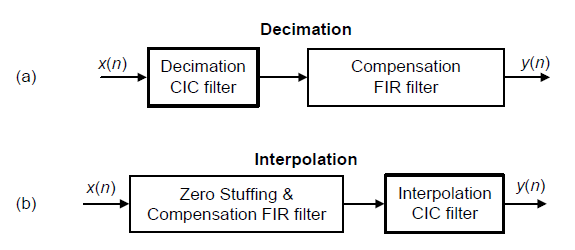
\includegraphics[width=0.8\textwidth]{images/CIC_Filter/CIC_digital_filters_fig1.png}
    \caption{CIC filter applications: (a) for decimation; (b) for interpolation.}
    \label{fig:cic_fig1}
\end{figure}
Because their frequency magnitude responses are sin(x)/x-like, CIC filters are typically followed, or preceded, by linear-phase lowpass tapped-delay line finite impulse response (FIR) filters whose tasks are to compensate for the CIC filter's non-flat passband. 

The \autoref{fig:cic_fig1} cascaded-filter architectures have valuable benefits. For example:
\begin{itemize}
    \item The FIR filters operate at reduced clock rates minimizing power consumption in high-speed hardware applications 
    \item CIC filters are popular in hardware devices; they need no filter coefficient data storage and require no multiplications. The arithmetic needed to implement CIC filters is strictly additions and subtractions only.
    \item Narrowband lowpass filtering can be attained at a greatly reduced computational complexity compared to using a single lowpass FIR filter. And this property is why CIC filters are so attractive in decimating and interpolating DSP systems.
\end{itemize}
\subsection{Recursive Running Sum Filter}
CIC filters originate from the notion of a recursive running sum filter, which is itself an efficient form of a nonrecursive moving averager. Recall the standard D-point moving-average process in \autoref{fig:cic_fig2}(a). There we see that D-1 summations (plus one multiply by 1/D) are necessary to compute the averager's y(n) output sequence.
\begin{figure}[!ht]
    \centering
    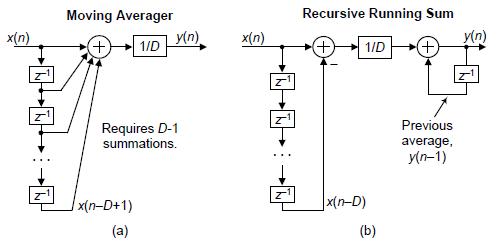
\includegraphics[width=0.8\textwidth]{images/CIC_Filter/CIC_digital_filters_fig2.png}
    \caption{D-point moving-average and recursive running sum filters.}
    \label{fig:cic_fig2}
\end{figure}
The D-point moving-average filter's time-domain output is expressed as 
\begin{equation}\label{eq:cic_1}
y(n)=\frac{1}{D}[x(n)+x(n-1)+x(n-2)+x(n-3)+\ldots+x(n-D+1)]
\end{equation}
where n is our time-domain index. The z-domain expression for this moving averager's output is 
\begin{equation}\label{eq:cic_2}
Y(z)=\frac{1}{D}\left[X(z)+X(z) z^{-1}+X(z) z^{-2}+\ldots+X(z) z^{-D+1}\right]
\end{equation}
while its z-domain $H_{\mathrm{MA}}(z)$ transfer function is 
\begin{equation}\label{eq:cic_3}
H_{\mathrm{MA}}(z)=\frac{Y(z)}{X(z)}=\frac{1}{D}\left[1+z^{-1}+z^{-2}+\ldots+z^{-D+1}\right]=\frac{1}{D} \sum_{n=0}^{D-1} z^{-n}
\end{equation}

We provide these equations not to make things complicated, but because they're useful. \autoref{eq:cic_1} tells us how to build a moving averager, and \autoref{eq:cic_3} is in the form used by commercial signal processing software to model the frequency-domain behavior of the moving averager. 


The next step in our journey toward understanding CIC filters is to consider an equivalent form of the moving averager, the recursive running sum filter depicted in Figure 2(b). Ignoring the 1/D scaling, there we see that the current input sample x(n) is added to, and the oldest input sample x(n-D) is subtracted from, the previous output average y(n-1). It's called 'recursive' because it has feedback. Each filter output sample is retained and used to compute the next output value. The recursive running sum filter's difference equation is

\begin{equation}\label{eq:cic_4}
y(n)=\frac{1}{D}[x(n)-x(n-D)]+y(n-1)
\end{equation}
having a z-domain $H_{\mathrm{RRS}}(z)$ transfer function of 
\begin{equation}\label{eq:cic_5}
H_{\mathrm{RRS}}(z)=\frac{Y(z)}{X(z)}=\frac{1}{D} \cdot \frac{1-z^{-D}}{1-z^{-1}}
\end{equation}

We use the same H(z) variable for the transfer functions of the moving average filter and the recursive running sum filter because their transfer functions are equal to each other! It's true. \autoref{eq:cic_3} is the nonrecursive expression, and \autoref{eq:cic_5} is the recursive expression, for a D-point averager. The mathematical proof of this can be found in Appendix B of Reference [1], but shortly I'll demonstrate that equivalency with in example. 

Here is why we care about recursive running sum filters: the standard moving averager in \autoref{fig:cic_fig2}(a) must perform D-1 additions per output sample. The recursive running sum filter has the sweet advantage that only one addition and one subtraction are required per output sample, regardless of the delay length D! This computational efficiency makes the recursive running sum filter attractive in many applications seeking noise reduction through averaging. Next we'll see how a CIC filter is, itself, a recursive running sum filter. 

\subsection{CIC Filter Structures}
If we condense the delay line representation and ignore the 1/D scaling in \autoref{fig:cic_fig2}(b) we obtain the classic form of a 1st-order CIC filter, whose cascade structure is shown in \autoref{fig:cic_fig3}.

\begin{figure}[!ht]
    \centering
    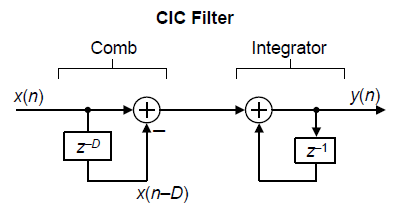
\includegraphics[width=0.8\textwidth]{images/CIC_Filter/CIC_digital_filters_fig3.png}
    \caption{D-point recursive running sum filter in a cascaded integrator-comb implementation.}
    \label{fig:cic_fig3}
\end{figure}

The feedforward portion of the CIC filter is called the comb section, whose differential delay is D, while the feedback section is typically called an integrator. The comb stage subtracts a delayed input sample from the current input sample, and the integrator is simply an accumulator. The CIC filter's time-domain difference equation is 
\begin{equation}
y(n)=x(n)-x(n-D)+y(n-1)
\end{equation}
and its z-domain transfer function is 
\begin{equation}
H_{\text {cIc }}(z)=\frac{Y(z)}{X(z)}=\frac{1-z^{-D}}{1-z^{-1}}
\end{equation}
To see why the CIC filter is of interest, first we examine its time-domain behavior, for D = 5, shown in \autoref{fig:cic_fig4}. If a unit impulse sequence, a unity-valued sample followed by many zero-valued samples, was applied to the comb stage, that stage's output is as shown in \autoref{fig:cic_fig4}(a). Think, now, what would be the output of the integrator if its input was the comb stage's impulse response. The initial positive impulse from the comb filter starts the integrator's all-ones output. Then, D samples later the negative impulse from the comb stage arrives at the integrator to zero all further CIC filter output samples. 

\begin{figure}[!ht]
    \centering
    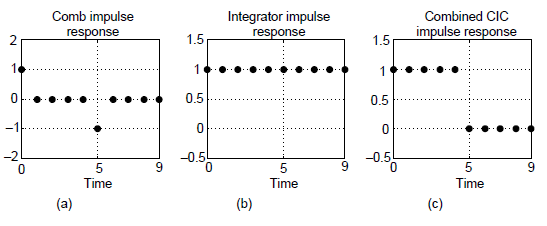
\includegraphics[width=0.8\textwidth]{images/CIC_Filter/CIC_digital_filters_fig4.png}
    \caption{Single-stage CIC filter time-domain responses when D = 5}
    \label{fig:cic_fig4}
\end{figure}

The key issue is that the combined unit impulse response of the CIC filter, being a rectangular sequence, is identical to the unit impulse responses of a moving average filter and the recursive running sum filter. (Moving averagers, recursive running sum filters, and CIC filters are close kin. They have the same z-domain pole/zero locations, their frequency magnitude responses have identical shapes, their phase responses are identical, and their transfer functions differ only by a constant scale factor.) If you understand the time-domain behavior of a moving averager, then you now understand the time-domain behavior of the CIC filter in \autoref{fig:cic_fig3}. 

The frequency magnitude and linear-phase response of a D = 5 CIC filter is shown in \autoref{fig:cic_fig5}(a) and \autoref{fig:cic_fig5}(b) where the frequency fs is the input signal sample rate measured in Hz.
\begin{figure}[!ht]
    \centering
    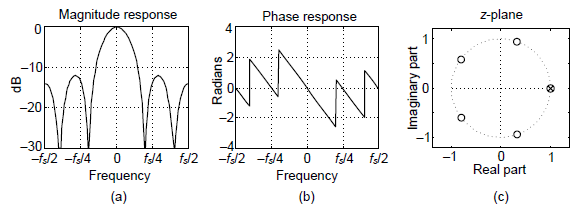
\includegraphics[width=0.8\textwidth]{images/CIC_Filter/CIC_digital_filters_fig5.png}
    \caption{Characteristics of a single-stage CIC filter when D = 5.}
    \label{fig:cic_fig5}
\end{figure}
The CIC filter's frequency response, derived in Reference [1], is: 
\begin{equation}\label{eq:cic8}
H_{\mathrm{CIC}}\left(e^{j 2 \pi f}\right)=e^{-j 2 \pi f(D-1) / 2} \cdot \frac{\sin (2 \pi f D / 2)}{\sin (2 \pi f / 2)}
\end{equation}
If we ignore the phase factor in \autoref{eq:cic8}, that ratio of sin() terms can be approximated by a sin(x)/x function. This means the CIC filter's frequency magnitude response is approximately equal to a sin(x)/x function centered at 0 Hz as we see in \autoref{fig:cic_fig5}(a). (This is why CIC filters are sometimes called sinc filters.)

Digital filter designers like to see z-plane pole/zero plots, so I provide the z-plane characteristics of a D = 5 CIC filter in \autoref{fig:cic_fig5}(C), where the comb filter produces D zeros, equally spaced around the unit-circle, and the integrator produces a single pole canceling the zero at $z=1$. Each of the comb's zeros, being a Dth root of 1, are located at $z(m)=e^{i 2 p m / D}$, where $m=0,1,2, \ldots, D-1$, corresponding to a magnitude null in \autoref{fig:cic_fig5}(a).

The normally risky situation of having a filter pole directly on the z-plane's unit circle need not trouble us here because there can be no coefficient quantization error in our $H_{\mathrm{CIC}(z)}$ transfer function. That's because CIC filter coefficients are ones and can be represented with perfect precision with fixed-point number formats. The filter pole will never be outside the unit circle. Although recursive, happily CIC filters are guaranteed-stable, linear-phase, and have finite-length impulse responses.

Again, CIC filters are primarily used for anti-aliasing filtering prior to decimation, and for anti-imaging filtering for interpolated signals. With those notions in mind we swap the order of \autoref{fig:cic_fig2}(C)'s comb and integrator-we're permitted to do so because those operations are linear-and include decimation by an integer sample rate change factor R in \autoref{fig:cic_fig6}(a). (The reader should prove to themselves that the unit impulse response of the integrator/comb combination, prior to the sample rate change, in \autoref{fig:cic_fig6}(a) is equal to that in \autoref{fig:cic_fig4}(C).) In most CIC filter applications the rate change R is equal to the comb's differential delay D, but I'll keep them as separate design parameters for now.

\begin{figure}[!ht]
    \centering
    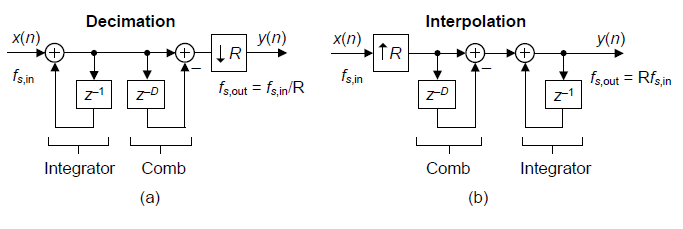
\includegraphics[width=0.8\textwidth]{images/CIC_Filter/CIC_digital_filters_fig6.png}
    \caption{Single-stage CIC filters used in (a) decimation and (b) interpolation. (Sample rates $f_{s,in}$ and $f_{s,out}$ are the sample rates of the x(n) and y(n) sequences respectively.)}
    \label{fig:cic_fig6}
\end{figure}

The decimation (also called 'down-sampling') operation $\downarrow$R means discard all but every Rth sample, resulting in an output sample rate of $f_{s,out}$ = $f_{s,in}$/R. To investigate a CIC filter's frequency-domain behavior in more detail, \autoref{fig:cic_fig7}(a) shows the frequency magnitude response of a D=8 CIC filter prior to decimation. The spectral band, of width B Hz, centered at 0 Hz is the desired passband of the filter. A key aspect of CIC filters is the spectral folding that takes place due to decimation.

\begin{figure}[!ht]
    \centering
    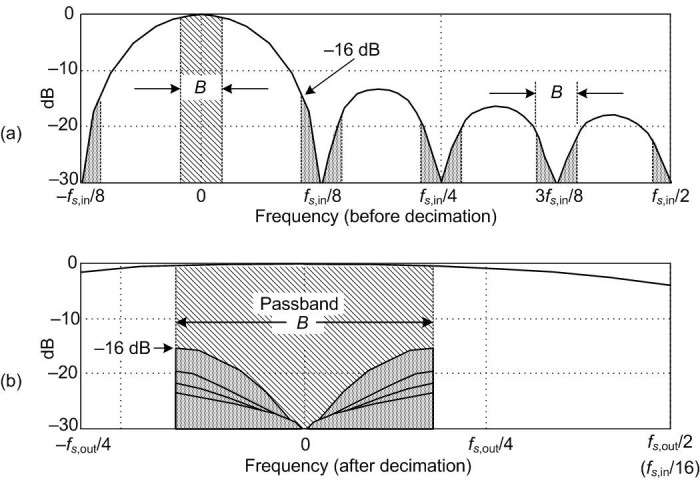
\includegraphics[width=0.8\textwidth]{images/CIC_Filter/fig 7_83485.jpg}
    \caption{Magnitude response of a 1st-order, D=8, decimating CIC filter: (a) before decimation; (b) aliasing after R=8 decimation. )}
    \label{fig:cic_fig7}
\end{figure}

Those B-width shaded spectral bands centered about multiples of fs,in/R in \autoref{fig:cic_fig7}(a) will alias directly into our desired passband after decimation by R = 8 as shown in \autoref{fig:cic_fig7}(b). Notice how the largest aliased spectral component, in this 1st-order CIC filter example, is 16 dB below the peak of the band of interest. Of course the aliased power levels depend on the bandwidth B; the smaller B the lower the aliased energy after decimation.

\autoref{fig:cic_fig6}(b) shows a CIC filter used for interpolation where the $\uparrow$R symbol means insert R-1 zeros between each x(n) sample (up-sampling), yielding a y(n)output sample rate of $f_{s,out}=R\cdot f_{s,in}$. (In this CIC filter discussion, interpolation is defined as zeros-insertion, called 'zero stuffing', followed by CIC filter lowpass filtering.)

To illustrate the spectral effects of interpolation by R=8, \autoref{fig:cic_fig8}(a) shows an arbitrary baseband spectrum, with its spectral replications, of a signal applied to the D=R=8 interpolating CIC filter of \autoref{fig:cic_fig6}(c). The interpolation filter's output spectrum in \autoref{fig:cic_fig8}(b) shows how imperfect CIC filter lowpass filtering gives rise to the undesired spectral images. 
\begin{figure}[ht]
    \centering
    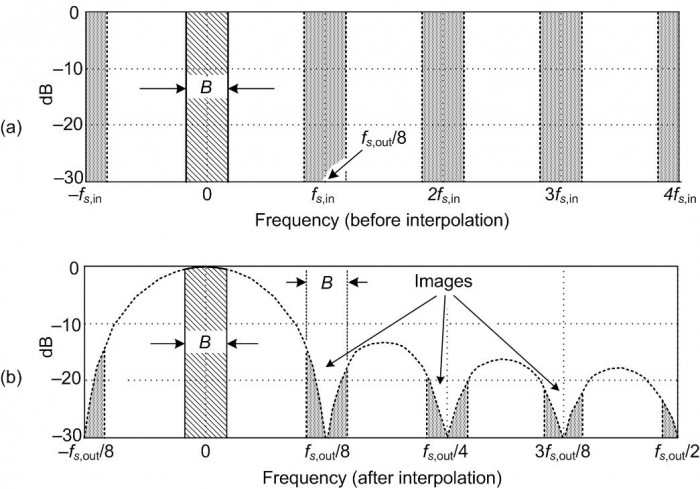
\includegraphics[width=0.8\textwidth]{images/CIC_Filter/fig 8_16431.jpg}
    \caption{1st-order, D=R=8, interpolating CIC filter spectra: (a) input signal spectrum; (b) spectral images of a zero stuffed and CIC lowpass filtered output.}
    \label{fig:cic_fig8}
\end{figure}

After interpolation, \autoref{fig:cic_fig8}(b) shows the unwanted images of the B-width baseband spectrum reside at the null centers, located at integer multiples of $f_{s,out}$/R. If we follow the CIC filter with a traditional lowpass tapped-delay line FIR filter, whose stopband includes the first image band, fairly high image rejection can be achieved.

\subsubsection{Comb Filters summary}
Moving average filter:
$$
H(z)=\sum_{k=0}^{M-1} z^{-k}
$$
This filter can also be written in IIR form which is the CIC filter:
$$
H(z)=\sum_{k=0}^{M-1} z^{-k}=\frac{1-z^{-M}}{1-z^{-1}}
$$
when using $z=\mathrm{e}^{j \omega T_s}$ we get the following result:
\begin{equation}\label{eq:CIC_filter_supression}
\begin{aligned}
H(f) &=\frac{1-\mathrm{e}^{-j \omega T_s \cdot M}}{1-\mathrm{e}^{-j \omega T_s}} \\
&=\frac{\mathrm{e}^{-j \frac{\pi f}{f_s} M}\left(\mathrm{e}^{j \frac{\pi f}{f_s} M}-\mathrm{e}^{-j \frac{\pi f}{f_s} M}\right)}{\mathrm{e}^{-j \frac{\pi f}{f_s}}\left(\mathrm{e}^{j \frac{\pi f}{f_s}}-\mathrm{e}^{-j \frac{\pi f}{f_s}}\right)} \\
&=\mathrm{e}^{-j \frac{\pi f}{f_s}(M-1)} \cdot \frac{\sin \left(\frac{\pi f}{f_s} M\right)}{\sin \left(\frac{\pi f}{f_s}\right)}
\end{aligned}
\end{equation}
When one cascades the filter, one gets the following formula: $Rightarrow$ The benefit is that one has more attenuation.
$$
H(z)=\left(\frac{1-z^{-M}}{1-z^{-1}}\right)^n
$$
With the command \mintinline[bgcolor=black]{matlab}{filterDesigner} one can open the filter Designer where one can set poles and zeros.\newline
\begin{listing}[!ht]
\begin{minted}[
frame=lines,
framesep=2mm,
baselinestretch=1.2,
bgcolor=black,
fontsize=\footnotesize,
linenos,
breaklines
]{matlab}
clc
clear
close all;
h_en = [1 -1];
impz(h_en,1,10);    %h_en = numerator, 1 = denumerator, 10 number of samples for impulse response
title({'\fontsize{14}{0}\selectfont Impulse Response','\fontsize{12}{0}\selectfont $X(z)=1-z^{-1}$'},'interpreter','latex');
[hz1, hp1, ht1] = zplane(h_en,1);%with the unit circle
set(findobj(hz1, 'Type', 'line'), 'Color', 'b','LineWidth',2); 
set(findobj(hp1, 'Type', 'line'), 'Color', [0, 0.7, 0],'LineWidth',2);
saveas(gcf,'C:\Users\...\impulse_response_1','epsc')

clc
[hz1, hp1, ht1] = zplane(h_en,1);%with the unit circle
set(findobj(hz1, 'Type', 'line'), 'Color', 'b','LineWidth',2); 
set(findobj(hp1, 'Type', 'line'), 'Color', [0, 0.7, 0],'LineWidth',2);
title({'\fontsize{14}{0}\selectfont Pole-Zero plot','\fontsize{12}{0}\selectfont $X(z)=1-z^{-1}=\frac{z-1}{z}$'},'interpreter','latex');
saveas(gcf,'C:\Users\...\pole_zero_1','epsc')

clc
freqz(h_en,1);
title({'Frequency response','$X(z)=1-z^{-1}$'},'interpreter','latex');
ax1 = gca; % current axes
ax1.Position(4) = ax1.Position(4)*.80; 
saveas(gcf,'C:\Users\...\freq_res_1','epsc')
\end{minted}
\end{listing}
\begin{figure}
\centering
\begin{subfigure}{.5\linewidth}
\centering
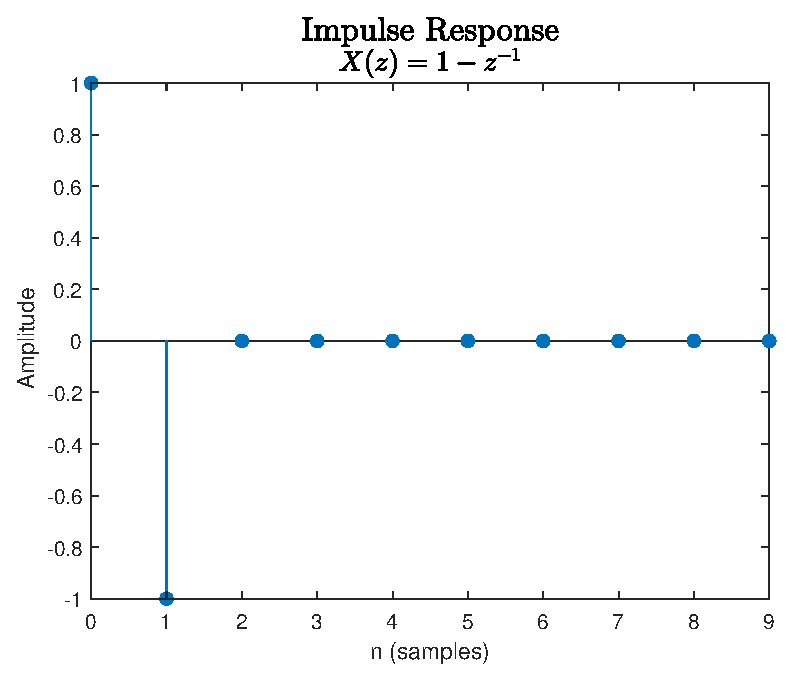
\includegraphics[scale=0.45]{images/impulse_response_1.eps}
\caption{}
\label{fig:sub1}
\end{subfigure}%
\begin{subfigure}{.5\linewidth}
\centering
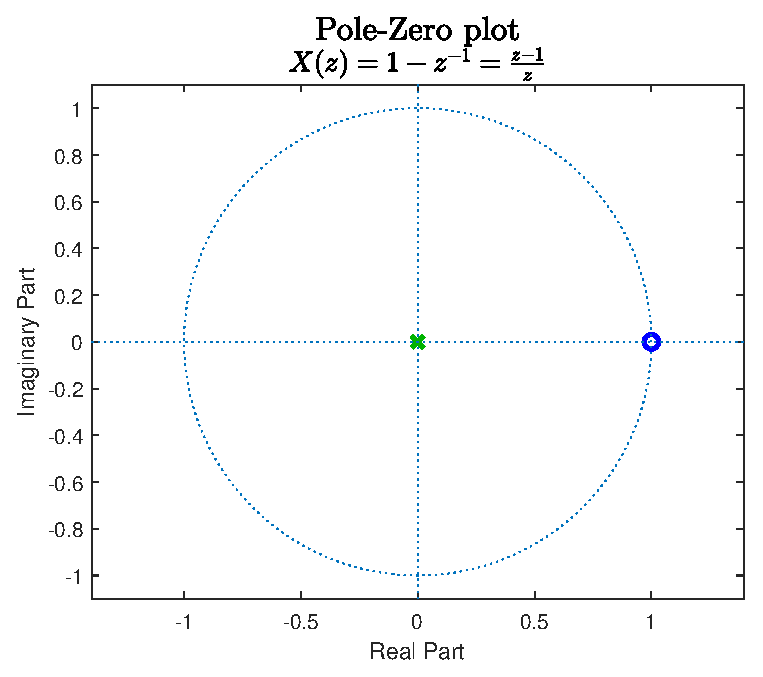
\includegraphics[scale=0.45]{images/pole_zero_1.eps}
\caption{}
\label{fig:sub2}
\end{subfigure}\\[1ex]
\begin{subfigure}{\linewidth}
\centering
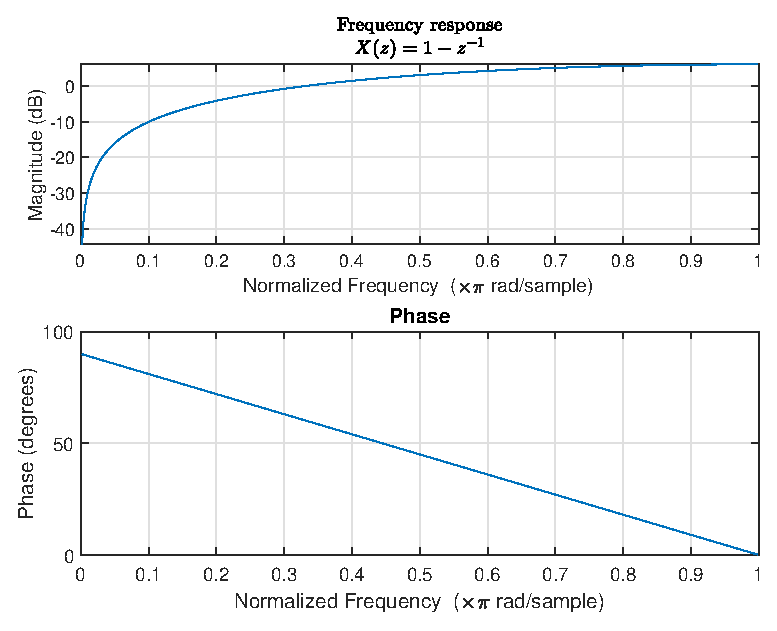
\includegraphics[scale=0.9]{images/freq_res_1.eps}
\caption{}
\label{fig:sub3}
\end{subfigure}
\caption{FIR filter}
\label{fig:test}
\end{figure}

\begin{figure}
\centering
\begin{subfigure}{.5\linewidth}
\centering
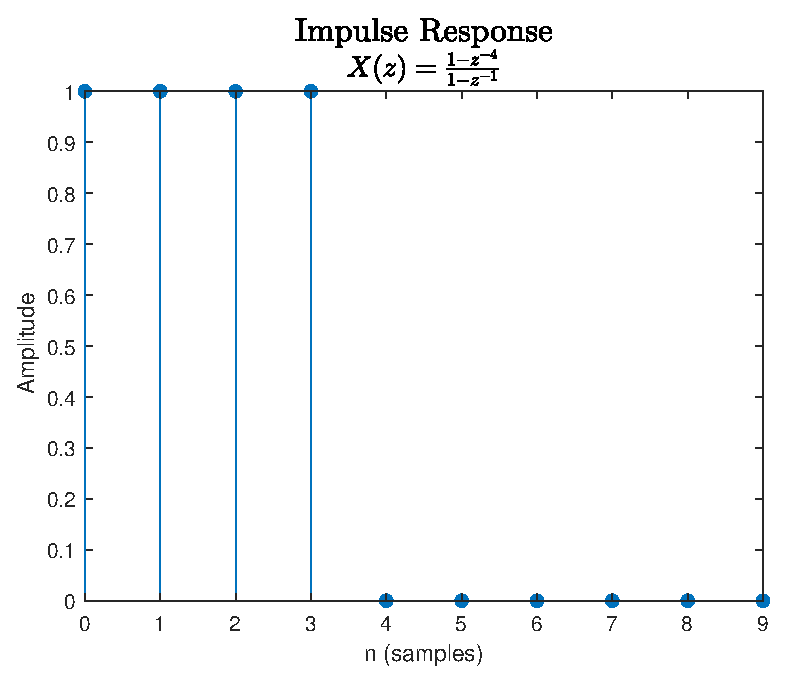
\includegraphics[scale=0.45]{images/impulse_response_2.eps}
\caption{}
\label{fig:sub1}
\end{subfigure}%
\begin{subfigure}{.5\linewidth}
\centering
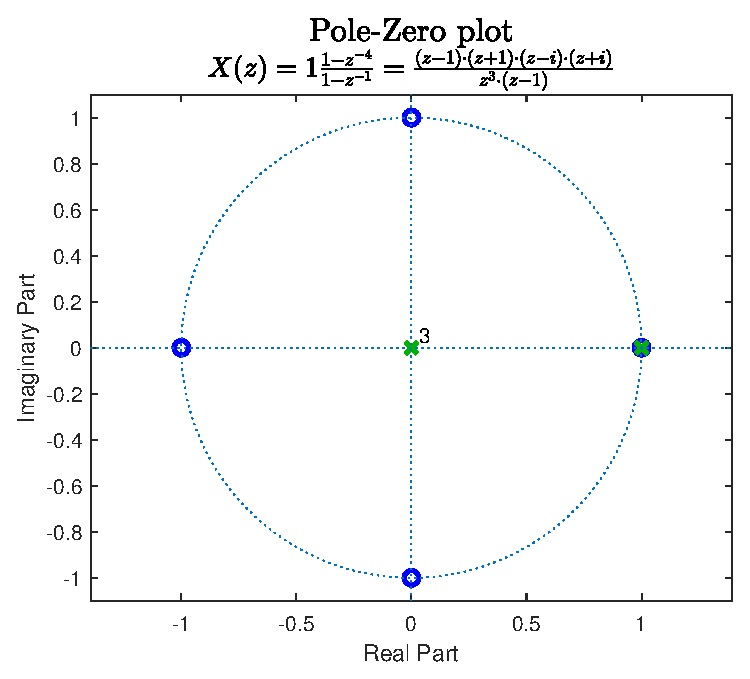
\includegraphics[scale=0.45]{images/pole_zero_2.eps}
\caption{}
\label{fig:sub2}
\end{subfigure}\\[1ex]
\begin{subfigure}{\linewidth}
\centering
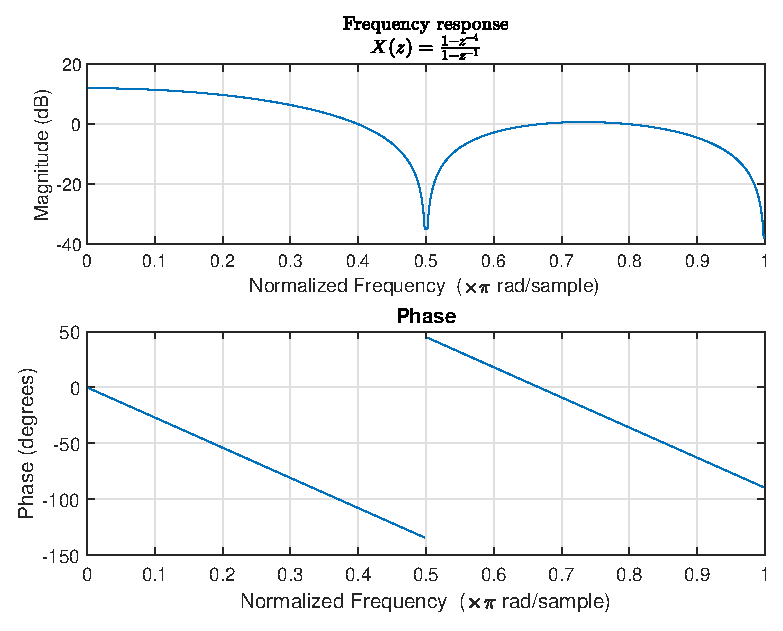
\includegraphics[scale=0.9]{images/freq_res_2.eps}
\caption{}
\label{fig:sub3}
\end{subfigure}
\caption{CIC filter with $M=4$, \textcolor{green}{Poles},\textcolor{blue}{Zeros}}
\label{fig:comp_filter_4}
\end{figure}


% \begin{figure}
%     \centering
%     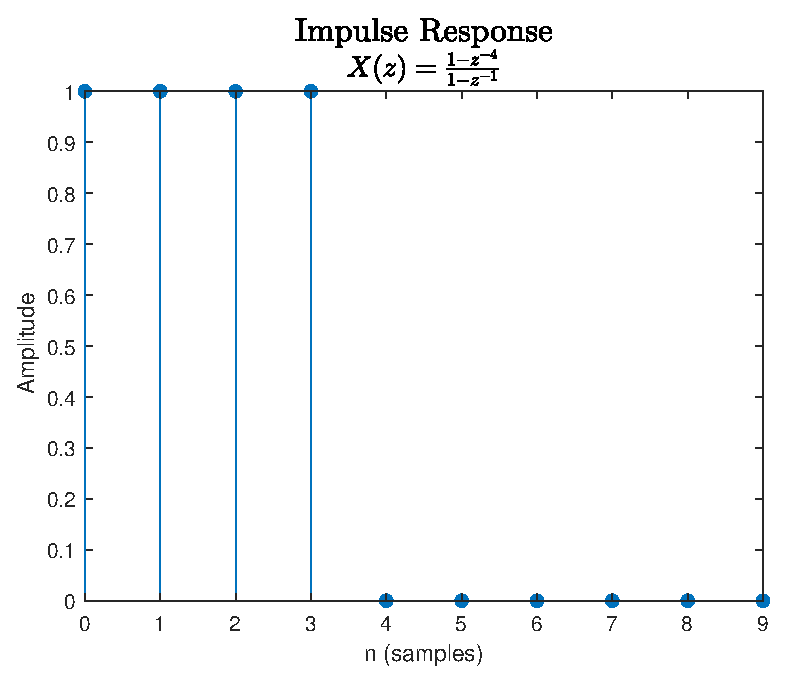
\includegraphics[scale=0.8]{images/impulse_response_2.eps}
%     \caption{Caption}
%     \label{fig:my_label}
% \end{figure}
% \begin{figure}
%     \centering
%     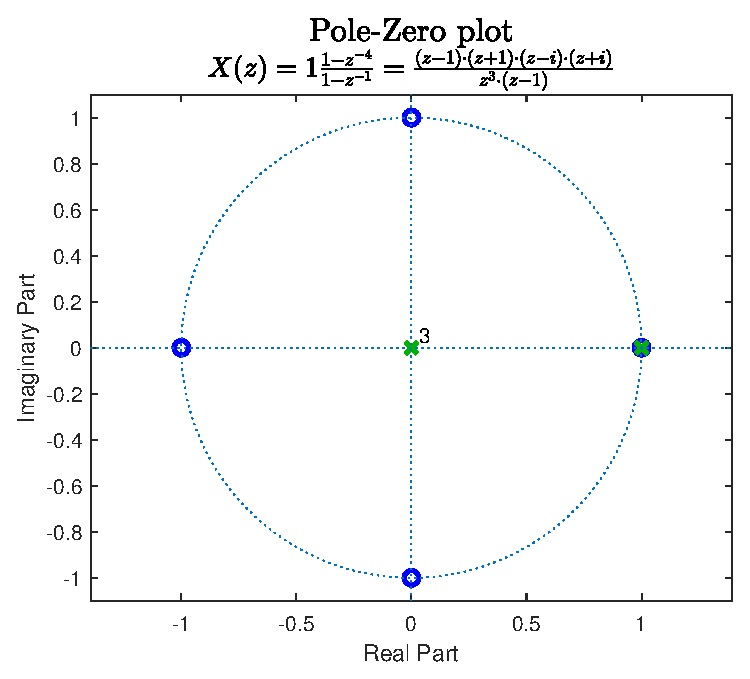
\includegraphics[scale=0.8]{images/pole_zero_2.eps}
%     \caption{Caption}
%     \label{fig:my_label}
% \end{figure}
% \begin{figure}
%     \centering
%     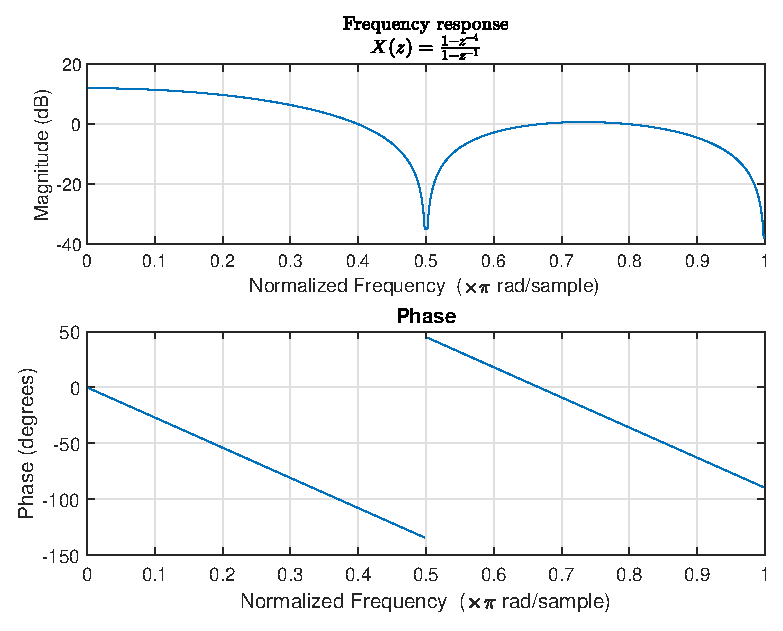
\includegraphics[scale=1]{images/freq_res_2.eps}
%     \caption{Caption}
%     \label{fig:my_label}
% \end{figure}
\FloatBarrier
\subsubsection{Exercise CIC filter}
In a digital receiver, the baseband signal is sampled with  $f_s = \SI{100}{\mega\hertz}$. To reduce the signal processing load
of the following stages, you design a CIC filter with M = 5 to bring the sampling rate down to $\SI{20}{\mega\hertz}$. The
corner frequency of the band of interest is at $f_c = \SI{5}{\mega\hertz}$.
\begin{itemize}
    \item At which frequency does the largest possible aliasing interfering with the band of interest occur? (Assuming white noise outside the band of interest.)\newline
    The largest alias occurs at the first aliasing frequency of the passband corner frequency $f_c$, i.e. $f_{a, \max }=\frac{f_s}{M}-f_c=15 \mathrm{MHz}$ (Since we downsample with a factor of five, our new sampling rate is 20MHz $\Rightarrow$ The frequency of 15MHz is read as the same as the frequency of 5MHz, 25MHz would also be an alias frequency, but is allready damped more)
    
    \item What is the minimum order n of the CIC filter to achieve an alias suppression greater than 40 dB?
    According to \autoref{eq:CIC_filter_supression} the following holds: $H(f)=e^{-j \frac{\pi f}{f_s} n(M-1)} \cdot\left(\frac{\sin \left(\frac{\pi f}{f_s} M\right)}{M \sin \left(\frac{\pi f}{f_s}\right)}\right)^n$. When one says that $H(f)$ at $f_a$ must be -40 db one gets the following for n: 
    $$\text{solve} \left(\left| e^{-j \frac{\pi \SI{15}{\mega\hertz}}{\SI{100}{\mega\hertz}} n(5-1)} \cdot\left(\frac{\sin \left(\frac{\pi \SI{15}{\mega\hertz}}{\SI{100}{\mega\hertz}} 5\right)}{5 \sin \left(\frac{\pi \SI{15}{\mega\hertz}}{\SI{100}{\mega\hertz}}\right)}\right)^n\right| = 10^{\frac{-40}{20}}\text{, n} \right)\Rightarrow n=3.94$$ Therefore the Order must be at least 4.
    \item How large is the passband droop for a filter of this order at $f_c$?\newline
    The drop at the passband is $\left| e^{-j \frac{\pi \SI{5}{\mega\hertz}}{\SI{100}{\mega\hertz}} n(5-1)} \cdot\left(\frac{\sin \left(\frac{\pi \SI{5}{\mega\hertz}}{\SI{100}{\mega\hertz}} 5\right)}{5 \sin \left(\frac{\pi \SI{5}{\mega\hertz}}{\SI{100}{\mega\hertz}}\right)}\right)^n\right|=0.668\Rightarrow 20\cdot \log_{10} 0.668=-3.5dB=H(f_c)$
\end{itemize}



\section{SW 2 Detection Theory}
When one transmits data over a non ideal channel, the output data is not the same anymore, which means the data could look completely different.  But to still reconstruct the correct data a detection algorithm on the output of the channel is needed to decide which data was originally sent. This page will have a look into this detection algorithm and how one can calculate how big the probability is that our detection algorithm is wrong.
\section{Additive White Gaussian Noise (AWGN)}
When we transmit a signal over a channel it is most probably that AWGN is added to our signal because we have thermal noise in our channel.
\subsection{Thermal noise}
Thermal noise occurs due to the vibration of charge carriers within an electrical conductor and is directly proportional to the temperature, regardless of the applied voltage.
AWGN ($n(t)$) which is also called a normal distribution, Gaussian or Gauss distribution with a mean ($\mu$) of zero and a variance of $\sigma^2$ can be described with the following probability density function:
\begin{equation}\label{eq:gauss_distribution_white noise}
p(n)=\frac{1}{\sigma \sqrt{2 \pi}} e^{-n^2 / 2 \sigma^2}
\end{equation}
\begin{equation}\label{eq:gauss_distribution}
p(x)=\frac{1}{\sigma \sqrt{2 \pi}} e^{-\frac{1}{2}(\frac{x-\mu}{\sigma})^2}
\end{equation}
The function says that the probability is very high, that we measure a signal that has a value close to zero ($n(t)$ has zero mean) and very low that we measure a value that is very far away from zero. 
\subsection{Probability}
The probability that we measure a certain value can be calculating by integrating the Gaussian function. But for this it is important to know that the cumulative distribution function (\href{https://en.wikipedia.org/wiki/Cumulative_distribution_function}{CDF}) of the standard normal distribution, usually denoted with the capital Greek letter $\Phi$ is not \href{https://en.wikipedia.org/wiki/Elementary_function}{elementary}, which means it's integral can not be described with a normal function. Therefore, often the \href{https://en.wikipedia.org/wiki/Q-function#Bounds_and_approximations}{Q-Function} is used to calculate the probability (a certain area below the function/ the integral with defined boundaries). Note that the q-function is the probability that a normal (Gaussian) random variable will obtain a value larger than $x$ standard deviations. The value of Q(x) can normally be looked up in tables, whereas gaussian distribution functions with a mean other than zero and a variance different from one can be not.
$$
Q(x)=\frac{1}{\sqrt{2 \pi}} \int_x^{\infty} \exp \left(-\frac{u^2}{2}\right) d u
$$
\begin{figure}[ht]
  \centering
  \resizebox{10cm}{!}{\subimport{images/}{probability1.tex}}
  %\includestandalone[width=1\linewidth]{wiener3.tex} % without the `.tex` extension
  \caption{Probability}
  \label{fig:probability1}
\end{figure}
Furthermore white noise is uncorrelated which means the autocorrelation plot is a dirac function.
\subsection{Bayes Law}
To calculate the BER or SER it is important to understand Bayes Law. Therefore, one finds an introduction to it in this section.
\begin{equation}
p(B) p(A \mid B)=p(B \mid A) p(A)
\end{equation}
Or in our application:
\begin{equation} \label{eq:map_1}
p\left(s_i \mid z\right)=\frac{\textcolor{blue}{p\left(z \mid s_i\right)} \textcolor{olive}{p\left(s_i\right)}}{\textcolor{violet}{p(z)}}
\end{equation}
\begin{itemize}
\item $\textcolor{olive}{p\left(s_i\right)\text{ a priori probability}}$
\item $\textcolor{blue}{p\left(z \mid s_i\right)\text{conditional probability or Likelihood}}$
\item $\textcolor{violet}{{p(z)}\text{ a poster priori probability}}$
\end{itemize}
\subsubsection{priori information}
$p(s_i)$ is the "a priori" probability that $s_i$ is sent. It is a feature of the data and not of the transmission, furthermore it is not always known. \newline
When one has this probability, it can be used to make a decision. For example, when we transmit language, the probability of sending a "q" is very low, but the probability of sending an "i" is much higher.

$\textcolor{blue}{p\left(z \mid s_i\right)}$, is a conditional probability: the probability of event z occurring given that $s_i$ is true. It is also called the posterior probability of z given $s_i$. In words, it says when we send signal $s_i$ the probability is $\textcolor{blue}{p\left(z \mid s_i\right)}$ to receive z. 
\subsubsection{Example}
10\% of the accidents is caused by drunk drivers $P(drunk \mid acc)=0.1$, The rest of the accident is caused by not drunk drivers $P(sober \mid acc)=0.9$ Which says ten precent of the accidents is cause by drunk drivers and 90\% of the accidents is caused by sober drivers, which could lead to the conclusion that one should be drunk when driving a car. Which is actually not true. Lets further assume that the probability of making an accident is $p(\operatorname{accident})=10^{-6}$ and the probability of being drunk is $p(drunk)=0.1$ and of being sober is $p(drunk)=0.9$. With bayes law we can now calculate what the probability of having an accident while being drunk is.

$$
p\left(\operatorname{accident} \mid p(drunk)\right)=\frac{p\left(p(drunk)\mid \text { accident }\right) \cdot p(\operatorname{accident})}{p(drunk)}=\frac{10^{-1} \cdot 10^{-6}}{10^{-2}}=10^{-5}
$$
$$
p\left(\operatorname{accident} \mid p(sober)\right)=\frac{p\left(p(sober)\mid \text { accident }\right) \cdot p(\operatorname{accident})}{p(sober)}=\frac{0.9 \cdot 10^{-6}}{0.99}\approx 10^{-6}
$$

\subsubsection{MAP receiver (Considers probability)} 
$$
\frac{p\left(\boldsymbol{r} \mid H_1\right)}{p\left(\boldsymbol{r} \mid H_0\right)}\underset{\substack{H_0}}{\stackrel{H_1}{\gtrless}} \frac{P_0}{P_1}
$$
This is also what one can see in \autoref{fig:probability_9}.
\begin{itemize}
\item Maximizes "a posteriori" probability
\item Choose $s_i$ such that $p(s_i \mid z)$ is maximized(see equation \ref{eq:map_1}), for this $\textcolor{olive}{p\left(s_i\right)}$ must be known
\end{itemize}
\subsubsection{ML(Maximum Likelihood) receiver (Does not consider probability)} 
Is the same as the MAP but maximizes only $\textcolor{blue}{p\left(z \mid s_i\right)}$. When $\textcolor{olive}{p\left(s_i\right)}=1/M$ ML and MAP are the same. \newline
To sum it up, what we generally do is we look at the point we measured which probability density function has the higher probability or to which point we are closer. The integral under the curve to the point also gives us the probability that our assumption was wrong.
\begin{figure}[ht]
  \centering
  \resizebox{10cm}{!}{\subimport{images/}{probability2.tex}}
  \caption{Probability2}
  \label{fig:probability_2}
\end{figure}
\section{Bit-error rate BER}
There are different ways to find out the error rates: (When confused about SER and BER watch the following  \href{https://youtu.be/du-sExIUV-Y}{video})
\begin{itemize}
\item Build the system and measure it $\Rightarrow$ this method is very time consuming and one has to build the real system
\item Monte-Carlo simulations $\Rightarrow$ this is even more time consuming, since the simulation is normally not as fast as the real application.
\item Analytic (numerical) solution $\Rightarrow$ this is very difficult to solve in certain cases
\end{itemize}

\subsubsection{Exercise Binary maximum-likelihood and MAP detection}
A random variable $X$ takes on the values 0 and 1 with the probabilities $P(X=0)=0.2$ and $P(X=1)=0.8$. A second random variable $Y$ has a Gaussian probability density function with mean $m=0$ and standard deviation $\sigma=1$. Our observation is the sum $Z=X+Y$.
\begin{enumerate}
    \item Determine and draw $p(z \mid X=0)$ and $p(z \mid X=1)$.\newline
    When X is zero Z must be Y, and therefore $p(z \mid X=0)=\frac{1}{\sqrt{ } 2 \pi} e^{-\frac{z^2}{2}}$. When X is one Z is 1+Y and therefore $p(z \mid X=1)=\frac{1}{\sqrt{2 \pi}} e^{-\frac{(z-1)^2}{2}}$
    \begin{figure}[ht]
      \centering
      \resizebox{8cm}{!}{\subimport{images/}{probability9.tex}}
      \caption{Probability9}
      \label{fig:probability_9}
    \end{figure}
    \item Use the maximum $a$-posteriori detection (MAP) to decide on the value of $X$, if $z=0.1$ was observed.\newline
    From \autoref{eq:gauss_distribution} one knows that $p(x)=\frac{1}{\sigma \sqrt{2 \pi}} e^{-\frac{1}{2}(\frac{x-\mu}{\sigma})^2}=\frac{1}{1 \sqrt{2 \pi}} e^{-\frac{1}{2}(\frac{0.1-0}{1})^2}$

    $$
    \begin{aligned}
    & X=0 \quad \Rightarrow \quad p(0.1 \mid X=0) \cdot P(X=0)=\frac{1}{\sqrt{2 \pi}} e^{-\frac{0.1^2}{2}} \cdot 0.2 \approx 0.079 \\
    & X=1 \quad \Rightarrow \quad p(0.1 \mid X=1) \cdot P(X=1)=\frac{1}{\sqrt{2 \pi}} e^{-\frac{(0.1-1)^2}{2}} \cdot 0.8 \approx 0.213
    \end{aligned}
    $$
    \begin{figure}[ht]
      \centering
      \resizebox{8cm}{!}{\subimport{images/}{probability10.tex}}
      \caption{Probability10}
      \label{fig:probability_10}
    \end{figure}
    Therefore we would decide for X=1 (this probability was higher)
    \item What would the decision be if you used maximum likelihood detection (ML)?\newline
    $$
    \begin{aligned}
    & X=0 \quad \Rightarrow \quad p(0.1 \mid X=0)=\frac{1}{\sqrt{2 \pi}} e^{-\frac{0.1^2}{2}} \approx 0.397 \\
    & X=1 \quad \Rightarrow \quad p(0.1 \mid X=1)=\frac{1}{\sqrt{2 \pi}} e^{-\frac{(0.1-1)^2}{2}} \approx 0.266
    \end{aligned}
    $$
    Therefore one would decide for X=0.
    \item Below which threshold of the observation value $z$ should you decide in favor of $X=0$ using MAP detection?\newline
    $$
    \begin{aligned}
    p(z \mid X=0) \cdot P(X=0) & >p(z \mid X=1) \cdot P(X=1) \\
    \frac{1}{\sqrt{2 \pi}} e^{-\frac{z^2}{2}} \cdot 0.2 & >\frac{1}{\sqrt{2 \pi}} e^{-\frac{(z-1)^2}{2}} \cdot 0.8 \\
    \frac{e^{-\frac{z^2}{2}}}{e^{-\frac{(z-1)^2}{2}}} & >\frac{0.8}{0.2} \\
    e^{-\frac{2 z-1}{2}} & >4 \\
    \frac{1-2 z}{2} & >\ln (4) \\
    z & <\frac{1}{2}-\ln (4)=-0.886
    \end{aligned}
    $$
    This is also what one can see in \autoref{fig:probability_10}.
    \item Below which threshold of the observation value $z$ should you decide in favor of $X=0$ using ML detection?\newline
    $$
    \begin{aligned}
    p(z \mid X=0) & >p(z \mid X=1) \\
    \frac{1}{\sqrt{2 \pi}} e^{-\frac{z^2}{2}} & >\frac{1}{\sqrt{2 \pi}} e^{-\frac{(z-1)^2}{2}} \\
    \frac{e^{-\frac{z^2}{2}}}{e^{-\frac{(z-1)^2}{2}}} & >1 \\
    e^{-\frac{2 z-1}{2}} & >1 \\
    \frac{1-2 z}{2} & >0 \\
    z & <\frac{1}{2}
    \end{aligned}
    $$
    This is also what one can see in \autoref{fig:probability_9}.
\end{enumerate}



\subsection{Analytic Solution}
To get the BER in an analytical way, we must know the following. White noise has a Gaussian distribution, as mentioned above, which can be described in with the formulat mentioned in equation \ref{eq:gaussian}. The signal which we measure is a \href{https://en.wikipedia.org/wiki/Energy_(signal_processing)}{discrete time signal} which energy is given by equation \ref{eq:energy_discrete_time}.
\begin{equation} \label{eq:gaussian}
f(x)=\frac{1}{\sigma \sqrt{2 \pi}} e^{-\frac{1}{2}\left(\frac{x-\mu}{\sigma}\right)^2}
\end{equation}
\begin{equation} \label{eq:energy_discrete_time}
E_s=\langle x(n), x(n)\rangle=\sum_{n=-\infty}^{\infty}|x(n)|^2
\end{equation}
\subsubsection{BPSK}
When we use the equations above, we can calculate the BER for the BPSK signal. The amplitude of the original signal is $\sqrt{E_s}$ which is a constant. When we add white noise to our signal(which is a constant) the white noise gets shifted, which means $\mu$ the mean is not zero any more but $\sqrt{E_s}$ (The expected value when we do a measurement is now $\sqrt{E_s}$). Therefore the BER which is for binary signals the same as the symbol error rate (SER). Blow one can see the calculation of the probability of error also BER.
$$
\begin{aligned}
P_E &=\int_0^{\infty} p(x \mid s=-1) d x \\
&=\int_0^{\infty} \frac{1}{\sqrt{2 \pi} \sigma} \mathrm{e}^{-\frac{\left(x+\sqrt{E_S}\right)^2}{2 \sigma^2}} d x \\
&=\int_0^{\infty} \frac{1}{\sqrt{2 \pi} \sqrt{\frac{N_0}{2}}} \mathrm{e}^{-\frac{\left(x+\sqrt{E_S}\right)^2}{N_0}} d x \\
&=\int_{\sqrt{E_S}}^{\infty} \frac{1}{\sqrt{2 \pi} \sqrt{\frac{N_0}{2}}} \mathrm{e}^{-\frac{x^2}{N_0}} d x \\
&=Q\left(\sqrt{\frac{2 E_S}{N_0}}\right) .
\end{aligned}
$$
Which corresponds to the blue area in \autoref{fig:probability_3}.
\begin{figure}[ht]
  \centering
  \resizebox{10cm}{!}{\subimport{images/}{probability3.tex}}
  \caption{Probability3}
  \label{fig:probability_3}
\end{figure}
Furthermore the SNR(Signal to noise ratio) for BPSK is $\frac{E_s}{N_0}$, where $N_0$ is the energy of the white noise.
% <iframe src="https://www.youtube.com/embed/vtJ6mAy3xMc" title="YouTube video player" allow="accelerometer; autoplay; clipboard-write; encrypted-media; gyroscope; picture-in-picture" allowfullscreen="" width="560" height="315" frameborder="0"></iframe>
\subsubsection{QPSK}
To calculate the SER of QPSK it is important to know the following:
$$\cos(\ang{45})=\frac{1}{\sqrt{2}}$$
When we assume the the energy per bit is still $E_s$ the distance between two signals is in QPSK $\frac{\sqrt{E_s}}{\sqrt{2}}$ Due to that the probability that we measure a signal on the right side of the $x$-axis when we have sent the signal on the top right corner is $P\left(x>0 \mid s_0\right)$ ,which is given by the formula below. (The factor of two cancels out)
$$
P\left(x>0 \mid s_0\right)=1-Q\left(\sqrt{\frac{E_s}{N_0}}\right)
$$
This is the same probability as $P\left(y>0 \mid s_0\right)$, therefore the probability that we measure the correct signal is $P\left(x>0 \mid s_0\right) \cdot P\left(y>0 \mid s_0\right)= \left(1-Q\left(\sqrt{\frac{E_s}{N_0}}\right)\right)^2$ and therefore the SER is given by the following equation:
\begin{equation}\label{eq:symbol_error_rate_qpsk}
\mathrm{SER}=1-\left(1-Q\left(\sqrt{\frac{E_s}{N_0}}\right)\right)^2
\end{equation}
\begin{figure}[ht]
  \centering
  \resizebox{10cm}{!}{\subimport{images/}{probability4.tex}}
  \caption{Probability4}
  \label{fig:probability_4}
\end{figure}
\subsubsection{Exercise error Probability of QPSK}
\begin{enumerate}
    \item Derive the expression for the SER/BER of a QPSK signal. Hint: Assume the probability for an error in x or y direction to be independent.\newline
    From \autoref{eq:symbol_error_rate_qpsk} one knows that it is for QPSK $\mathrm{SER}=1-\left(1-Q\left(\sqrt{\frac{E_s}{N_0}}\right)\right)^2$. \newline But the derivation would be quite easy. The energy per symbol must be one. Therefore, the amplitude in x and y direction is $\frac{1}{\sqrt{2}}$ since $\sqrt{(\frac{1}{\sqrt{2}})^2+(\frac{1}{\sqrt{2}})^2}=1$ The probability that one makes an error of $p_a$ as it can be seen in \autoref{fig:qpsk_bit_error} is therefore defined as the following.
    $$
    p_a=P\left(x<0 \mid d_0\right) P\left(y>0 \mid d_0\right)=Q\left(\sqrt{\frac{E_s}{N_0}}\right)\left(1-Q\left(\sqrt{\frac{E_s}{N_0}}\right)\right)=Q\left(\sqrt{\frac{E_s}{N_0}}\right)-Q\left(\sqrt{\frac{E_s}{N_0}}\right)^2
    $$
    Since $P\left(x<0 \mid d_0\right)=Q\left(\sqrt{\frac{E_s}{N_0}}\right)$ and $p_b$ as the following:
    $$
    p_b=P\left(x<0 \mid d_0\right) P\left(y<0 \mid d_0\right)=\left(Q\left(\sqrt{\frac{E_s}{N_0}}\right)\right)^2
    $$
    $$
    \begin{aligned}
    \mathrm{BER}_{\mathrm{conv}} & =\frac{1}{2}\left(p_a \cdot(1+2)+p_b \cdot 1\right) \\
    \mathrm{BER}_{\mathrm{Gray}} & =\frac{1}{2}\left(p_a \cdot(1+1)+p_b \cdot 2\right)
    \end{aligned}
    $$
    \begin{figure}[ht]
      \centering
      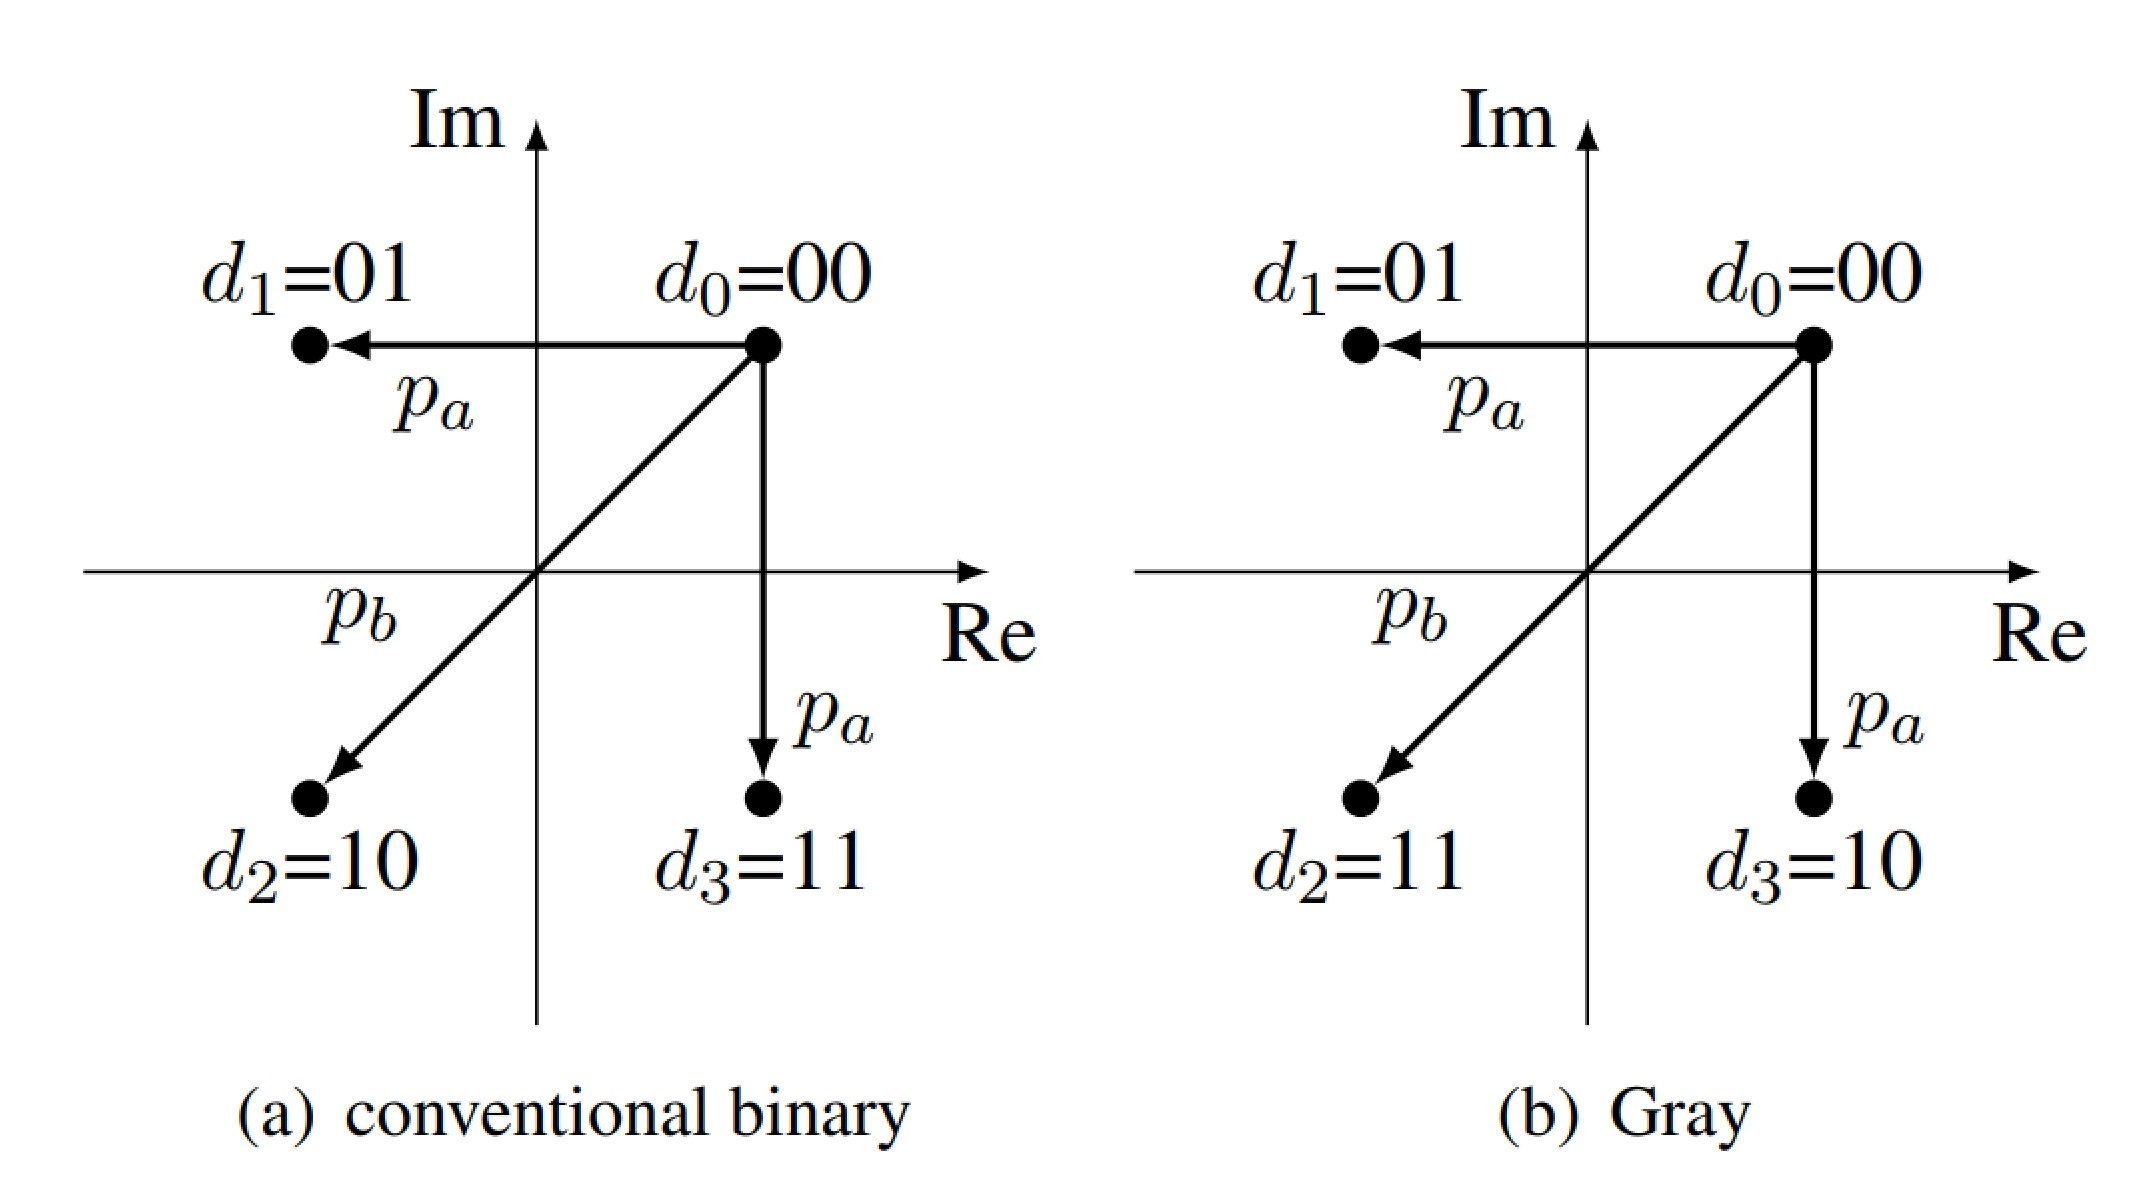
\includegraphics[width=10cm]{images/bit_error.jpg}
      \caption{Error}
      \label{fig:qpsk_bit_error}
    \end{figure}
    \item What difference in BER do we have between Gray code and conventional binary code?\newline
    $$
    \frac{\mathrm{BER}_{\text {conv }}}{\mathrm{BER}_{\mathrm{Gray}}}=\frac{3 p_a+p_b}{2 p_a+2 p_b}=\frac{3 Q(.)-3 Q^2(.)+Q^2(.)}{2 Q(.)-2 Q^2(.)+2 Q^2(.)}=\frac{3-2 Q(.)}{2}
    $$
    For larger $\frac{E_s}{N_0}, Q(\cdot)$ becomes small and can be neglected, leading to
    $$
    \frac{\mathrm{BER}_{\text {conv }}}{\mathrm{BER}_{\mathrm{Gray}}} \approx \frac{3}{2} .
    $$
\end{enumerate}


\section{Signal Space}
A signal space is a vector space with finite dimension. The vectors $\left\{\psi_1(t), \psi_2(t), \ldots \psi_N(t)\right\}$ are orthagonal when the inner products between two different vectors is zero and with the same vector one. $\left\langle\psi_i(t), \psi_j(t)\right\rangle$ stands for the inner product of $psi_i(t)$ and $\psi_j(t)$.
$$
\begin{aligned}
&\left\{\psi_1(t), \psi_2(t), \ldots \psi_N(t)\right\} \\
&\left\langle\psi_i(t), \psi_j(t)\right\rangle= \begin{cases}1 & j=i \\
0 & j \neq i\end{cases}
\end{aligned}
$$
A signal vector is:
$$
s_i(t)=\sum_{j=1}^N a_{i, j} \psi_j(t)
$$
with
\begin{itemize}
\item $a_{i j}$ are the coefficients of $s_i(t)$ in signal space
\item $\underline{S}_i=\left[\begin{array}{ll}a_{i 1} & a_{i 2} \cdots a_{i N}\end{array}\right]$
\item $a_{i k}=\left\langle s_i(t), \psi_k(t)\right\rangle$
\item $\left\|s_i(t)\right\|^2=\sum_{j=1}^N a_{i j}^2$
\end{itemize}
To determine how efficient our protocol is one can calculate the average energy per symbol as below.
$$
E_s=\frac{1}{M} \sum_{i=1}^M\left\|s_i(t)\right\|^2
$$
\begin{itemize}
\item Transmitted signal $s_i(t)$
\item AWGN noise $\hat{n}(t)$
\item threshold $\gamma$
\item Received signal $r(t) = s_i(t) + \hat{n}(t)$
\item Filter output: $z(t)=r(t)*h(t)=s_i(t)*h(t)+\hat{n}(t)*h(t)=a_i(t)+n(t)$
\end{itemize}
$z(t)$ was at any point in time whereas $z(T)$ is at a specific sample point, when we sample once per symbol time T is the symbol time.
The last box in the plot above is the test statistic, dependent of the value of z it will say the signal is one or zero.\newline
When one sends symbol zero one receives the following without noise $a_0(T) = s_0(t)*h(t)\rvert_{t = T}$ and when sending symbol one the following $a_1(T) = s_1(t)*h(t)\rvert_{t = T}$. For the noise part one gets the following $n(T)=\hat(n)(t)*h(t)\rvert_{t = T}$, since our filter is linear, we get again a Gaussian process, so nothing changes. The Gaussian signal can be described with the following formula:
$$
n \sim N\left(0, \sigma^2\right)
$$
For the test statistic we get the following: $z(T)=a_i(T)+n(T)$ and since a Gaussian signal + a constant gives another gausian signal, but with another mean we can describe it like the following: $z(T)=N(a_i(T),\sigma^2)$
\subsection{conditional density}
\begin{itemize}
\item $p_z(z\rvert \text{i sent})$ probability density functen when i is sent
\item $p_z(z\rvert 0)$ probability density when 0 was sent
\item $Pr(s_i \rvert z)$ is the probability that the data sent was "i" given the test statistic is $z$
\end{itemize}
So the probability density function of $z(T)$ if "0" was sent is the following:
$$
\begin{aligned}
p_z(z \mid 0) &=p\left(z=a_0+n\right)=p_n\left(n=z-a_0\right) \\
&=\frac{1}{\sqrt{2 \pi} \sigma} e^{-\left(z-a_0\right)^2 / 2 \sigma^2}
\end{aligned}
$$
\begin{figure}[ht]
  \centering
  \resizebox{1\textwidth}{!}{\subimport{images/}{probability5.tex}}
  \caption{Probability5}
  \label{fig:probability_5}
\end{figure}
\begin{figure}[ht]
  \centering
  \resizebox{1\textwidth}{!}{\subimport{images/}{probability6.tex}}
  \caption{Probability6}
  \label{fig:probability_6}
\end{figure}
\section{Modulation Formats}
As one can see below, there are different types of modulations
\subsection{Vocabulary}
\begin{itemize}
\item bit $\Rightarrow$ is a binary bit logical one or zero
\item symbol $\Rightarrow$ Could include a larger number of bits, is sometimes also called waveform.
\item alphabet or constellation $\Rightarrow$ is a collection of symbols, the alphabet for a bit would be zero and one.
\begin{itemize}
\item Binary alphabet$\{0,1\}$
\item Tertiary alphabet $\{A,B,C\}$
\end{itemize}
\end{itemize}

In a digital communication system, we want to transmit something digitally, but normally the original signal is analog like voice, therefore one has to digitize it and afterwards to transmit it we normally put it into analog again, because normally one can not transmit the signal digitally.
\subsection{PCM pulse code modulation}
One transmits the original signal with multiple bits.
\subsubsection{Example}
I want to transmit the data from a 3bit ADC $\Rightarrow$ we have eight different codes. With this modulation we transmit three different bits.
\subsection{PAM pulse amplitude modulation}
One transmits the original signal with different amplitudes. Here we have a symbol rather than a binary bit.
\subsubsection{Example}
I want to transmit the data from a 3bit ADC $\Rightarrow$ we have eight different codes. To transmit this signal I generate 8 different amplitudes.
\subsection{Conclusion}
To transmit the same amount of data PCM must have much higher frequencies than PAM (in the example above it must be three times larger, because in the same amount of time we must transmit three bits) $\Rightarrow$ PCM uses a larger bandwidth. But there are a lot more line codes as can be seen blow and each one of those is good at a very specific thing. (Clock recovery, error detection, differential coding, etc.)
\subsection{criteria for a good communication system}
\begin{itemize}
\item Power efficiency $\Rightarrow$ Bit Error Rate (BER) vs SNR
\item Spectral efficiency $\Rightarrow$ $\eta=\frac{R_b}{B_s} \leftarrow$ system bit rate $/$ system BW 
\begin{itemize}
\item $R_b=\frac{1}{T_b} \quad, T_b$ : bit duration
\item $T_s$ : Symbol duration $=\left(\log _2 M\right) T_b$ 
\end{itemize}
$$B_S=B W \cong \frac{1}{T_S}$$
\item Cost/complexity
\end{itemize}

\section{Linear Sampling Receiver}
When we simplify the schematic above, we get a sampling receiver
\begin{figure}[ht]
  \centering
  \resizebox{1\textwidth}{!}{\subimport{images/}{probability7.tex}}
  \caption{Probability7}
  \label{fig:probability_7}
\end{figure}
\section{Optimum linear filters}
\subsection{Wiener Filtering}
A Wiener filter minimizes the mean-square error to a minimum.
\begin{figure}[ht]
  \centering
  \resizebox{1\textwidth}{!}{\subimport{images/}{wiener3.tex}}
  %\includestandalone[width=1\linewidth]{wiener3.tex} % without the `.tex` extension
  \caption{Wiener filter=FIR filter!}
  \label{fig:wiener_3}
\end{figure}
\begin{figure}[ht]
  \centering
  \resizebox{1\textwidth}{!}{\subimport{images/}{wiener4.tex}}
  %\includestandalone[width=1\linewidth]{wiener4.tex} % without the `.tex` extension
  \caption{Wiener filter overview}
  \label{fig:wiener_2}
\end{figure}
The output of the filter in the diagram above can be described as the following:
$$
    \hat{s}[n+D]=\sum_{i=0}^{M} \textcolor{orange}{w}_{i} \cdot \textcolor{blue}{y}[n-i]
$$
\begin{itemize}
    \item $\textcolor{orange}{\boldsymbol{w}}$ is called the weighting or coefficient vector $\boldsymbol{\textcolor{orange}{w}} \triangleq\left[\textcolor{orange}{w}_1, \textcolor{orange}{w}_2, \ldots, \textcolor{orange}{w}_N\right]^T$
    \item $\boldsymbol{\textcolor{violet}{s}}$ is the input signal vector $\boldsymbol{\textcolor{violet}{s}} \triangleq\left[\textcolor{violet}{s}_1, \textcolor{violet}{s}_2, \ldots, \textcolor{violet}{s}_k\right]^T$
    \item $\boldsymbol{\textcolor{violet}{\hat{s}}}$ is the output signal
    \item $\textcolor{blue}{y}[n]$ is the received signal
    \item $\boldsymbol{\textcolor{pink}{x}}$ is the input signal plus the channel behaviour
\end{itemize}
% One can rewrite this with a matrix $\boldsymbol{\textcolor{orange}{w}}^T$ $\boldsymbol{\textcolor{blue}{y}}[n]$:
Let's assume one has a filter with three filter coefficients $\textcolor{orange}{w}_0,\textcolor{orange}{w}_1,\textcolor{orange}{w}_2$. The output can then be written in the following form:
$$
\begin{aligned}
& \textcolor{violet}{\hat{s}}[0]=w_0 \textcolor{blue}{y}[0] \\
& \textcolor{violet}{\hat{s}}[1]=w_0 \textcolor{blue}{y}[1]+w_1 \textcolor{blue}{y}[0] \\
& \textcolor{violet}{\hat{s}}[2]=w_0 \textcolor{blue}{y}[2]+w_1 \textcolor{blue}{y}[1]+w_2 \textcolor{blue}{y}[0] \\
& \textcolor{violet}{\hat{s}}[3]=w_0 \textcolor{blue}{y}[3]+w_1 \textcolor{blue}{y}[2]+w_2 \textcolor{blue}{y}[1]
\end{aligned}
$$
Where $\boldsymbol{\textcolor{violet}{\hat{s}}}[k]$ can also be written as $\boldsymbol{A}[k] \boldsymbol{\textcolor{orange}{w}}$ where $\boldsymbol{A}[k]$ is the following:
$$
\boldsymbol{A}[k]=\left(\begin{array}{ccc}
\textcolor{blue}{y}[0] & 0 & 0 \\
\textcolor{blue}{y}[1] & \textcolor{blue}{y}[0] & 0 \\
\textcolor{blue}{y}[2] & \textcolor{blue}{y}[1] & \textcolor{blue}{y}[0] \\
\vdots & \vdots & \vdots \\
\textcolor{blue}{y}[k] & \textcolor{blue}{y}[k-1] & \textcolor{blue}{y}[k-2]
\end{array}\right)
$$
and $\boldsymbol{\textcolor{orange}{w}} \triangleq\left[\textcolor{orange}{w}_1, \textcolor{orange}{w}_2, \ldots, \textcolor{orange}{w}_N\right]^T$ the error can then be written as:
$$
e[k]=\boldsymbol{\textcolor{violet}{s}}[k]-\boldsymbol{\textcolor{blue}{y}}[k]=\boldsymbol{\textcolor{violet}{s}}[k]-\boldsymbol{A}[k] \boldsymbol{\textcolor{orange}{w}}[k]
$$
The error is minimized when the following condition is given:
$$
\boldsymbol{\textcolor{orange}{w}}[k]=\left(\boldsymbol{A}^T[k] \boldsymbol{A}[k]\right)^{-1} \boldsymbol{A}^T[k] \boldsymbol{\textcolor{violet}{s}}[k]
$$
% $$
%     \hat{s}[n]=\underbrace{\boldsymbol{w}^T}_{\text{row vector}} \cdot \overbrace{\textcolor{blue}{\boldsymbol{y}}[n]}^{\text{column vector}}
% $$
% where $\boldsymbol{w} \triangleq\left[w_1, w_2, \ldots, w_N\right]^T$ and $\textcolor{blue}{\boldsymbol{y}}[n] \triangleq[\textcolor{blue}{y}[n], \textcolor{blue}{y}[k-1], \ldots, \textcolor{blue}{y}[k-N+1]]^T$
% The error is then described with \autoref{eq:error}
% \begin{equation} \label{eq:error}
%     e[n]=\textcolor{violet}{\hat{s}}[n]-\textcolor{blue}{y}[n]=d[n]-\boldsymbol{w}^T \textcolor{blue}{\boldsymbol{y}}[n]
% \end{equation}
% But we are interested in the square error:
% $$
% \begin{aligned}
%     e^2[n] &=\left(d[n]-\boldsymbol{w}^T \textcolor{blue}{\boldsymbol{y}}[n]\right) \cdot\left(d[n]-\textcolor{blue}{\boldsymbol{y}}^T[n] \boldsymbol{w}\right) \\
%     &=d^2[n]+\boldsymbol{w}^T \textcolor{blue}{\boldsymbol{y}}[n] \textcolor{blue}{\boldsymbol{y}}^T[n] \boldsymbol{w}-2 d[n] \textcolor{blue}{\boldsymbol{y}}^T[n] \boldsymbol{w}
% \end{aligned}
% $$
% Note that $\textcolor{blue}{\boldsymbol{y}}^T[n] \boldsymbol{w}=\boldsymbol{w}^T \textcolor{blue}{\boldsymbol{y}}[n]$, since both are column vectors with the same size.
% To proceed further one must know that the follogin for the derivatives of vectors applies:
% $$
% \begin{aligned}
% \nabla \boldsymbol{v}\left\{\boldsymbol{u}^T \boldsymbol{v}\right\} &=\nabla \boldsymbol{v}\left\{\boldsymbol{v}^T \boldsymbol{u}\right\}=\boldsymbol{u} \\
% \nabla \boldsymbol{u}\left\{\boldsymbol{u}^T \boldsymbol{u}\right\} &=2 \boldsymbol{u} \\
% \nabla \boldsymbol{v}\left\{\boldsymbol{v}^T \boldsymbol{A}\right\} &=\boldsymbol{A} \\
% \nabla \boldsymbol{v}\left\{\boldsymbol{v}^T \boldsymbol{A} \boldsymbol{v}\right\} &=\boldsymbol{A} \boldsymbol{v}+\boldsymbol{A}^T \boldsymbol{v}
% \end{aligned}
% $$
% For symetric matrices the following applies:
% $$
% \nabla\boldsymbol{v}\left\{\boldsymbol{v}^T \boldsymbol{R} \boldsymbol{v}\right\}=2 \boldsymbol{R} \boldsymbol{v}
% $$
% And for transformation the following applies:
% $$
% (\boldsymbol{A} \boldsymbol{B})^T=(\boldsymbol{B})^T(\boldsymbol{A})^T
% $$
% $$
% (\boldsymbol{A}^T)^T=A
% $$
% With this we can write the estimation $E$ of the error with the following formula:
% $$
% E\left\{e^2[n]\right\}=E\left\{d^2[n]\right\}+\boldsymbol{w}^T E\left\{\textcolor{blue}{\boldsymbol{y}}[n] \textcolor{blue}{\boldsymbol{y}}^T[n]\right\} \boldsymbol{w}-2 E\left\{d[n] \textcolor{blue}{\boldsymbol{y}}^T[n]\right\} \boldsymbol{w}
% $$
% $$
% E\left\{e^2[n]\right\}=E\left\{d^2[n]\right\}+\boldsymbol{w}^T \boldsymbol{R} \boldsymbol{w}-2 \boldsymbol{p}^T \boldsymbol{w}
% $$
% The minimization of the mean-squared error according can be achieved by setting the differentiation
% of this quadratic equation with respect to the coefficient vector w equal to zero,
% $$
% \nabla_{\boldsymbol{w}}\left\{E\left\{e^2[n]\right\}\right\}=2 \boldsymbol{R} \boldsymbol{w}-2 \boldsymbol{p}
% $$
% When setting this equation now to zero, we get the following equation
% $$
% 2 \boldsymbol{R} \boldsymbol{w}=2 \boldsymbol{p}
% $$
% and the result of this equation is:
When rewriting this we end up with the following equation:
$$
\boldsymbol{w}_{\mathrm{MMSE}}=\boldsymbol{R}^{-1} \boldsymbol{p}
$$
which is also called the $\textbf{wiener-hopf equation}$. Also note that $\mathbf{R}$ is the autocorrelation with the input signal
$$
\mathbf{R}_{\textcolor{blue}{y y}}=\left(\begin{array}{cccc}
\gamma_{\textcolor{blue}{y y}}[0] & \gamma_{\textcolor{blue}{y y}}[-1] & \cdots & \gamma_{\textcolor{blue}{y y}}[-M] \\
\gamma_{\textcolor{blue}{y y}}[1] & \gamma_{\textcolor{blue}{y y}}[0] & \cdots & \gamma_{\textcolor{blue}{y y}}[1-M] \\
\vdots & \vdots & & \vdots \\
\gamma_{\textcolor{blue}{y y}}[M] & \gamma_{\textcolor{blue}{y y}}[M-1] & \cdots & \gamma_{\textcolor{blue}{y y}}[0]
\end{array}\right)
$$
and $\boldsymbol{p}$ or also $\mathbf{r}_{\textcolor{violet}{s} \textcolor{blue}{y}}$ the cross-correlation of the input and the chennel output.
$$
\mathbf{r}_{\textcolor{violet}{s} \textcolor{blue}{y}}=\left(\begin{array}{c}
\gamma_{\textcolor{violet}{s} \textcolor{blue}{y}}[D] \\
\gamma_{\textcolor{violet}{s} \textcolor{blue}{y}}[D+1] \\
\vdots \\
\gamma_{\textcolor{violet}{s} \textcolor{blue}{y}}[D+M]
\end{array}\right)
$$
\subsubsection{Exercise Wiener filter without white noise}
\begin{figure}[ht]
  \centering
  %\includestandalone[width=1\linewidth]{wiener_exercise.tikz} % without the `.tex` extension
  \resizebox{1\textwidth}{!}{\subimport{images/}{wiener_exercise.tex}}
  \caption{Wiener filter example}
  \label{fig:wiener_1}
\end{figure}
\paragraph{What is $h[n]$ of the first part in \autoref{fig:wiener_1}?}\mbox{}\newline
\autoref{fig:wiener_1} shows that the first part is an IIR Filter with $h[n]=\alpha^n \cdot \epsilon[n]$
\paragraph{Lets assume $\alpha$ is -0.5. How does $H[z]$ and it's inverse look like?}
We know the following:\newline
\begin{minipage}{\textwidth}
\begin{align*}
h\tikzmark{xx}(n)&= \alpha^n\cdot\tikzmark{yy}\epsilon[n] \\[2em]
X(z) &= \frac{z}{z-a}
\end{align*}

\begin{tikzpicture}[overlay,remember picture, > = {Circle[open,blue]}]
  \draw [<->] ([yshift=-.7ex]pic cs:xx) -- ++(0,-2.2em);
  \draw [<->] ([yshift=-.7ex]pic cs:yy) -- ++(0,-2.2em);
\end{tikzpicture}
\end{minipage}
Therefore $X(z)=\frac{1}{1-\alpha \cdot z^{-1} }$ and $X(z)^{-1}=1-\alpha \cdot z^{-1}$\newline
\begin{minipage}{\textwidth}
\begin{align*}
X\tikzmark{x}(z)^{-1}&= 1-\alpha\cdot\tikzmark{y}z^{-1} \\[2em]
h^{-1}[n] &= 1\cdot\delta[n]-\alpha\cdot \delta[n-1]
\end{align*}

\begin{tikzpicture}[overlay,remember picture, > = {Circle[open,blue]}]
  \draw [<->] ([yshift=-.7ex]pic cs:x) -- ++(0,-2.2em);
  \draw [<->] ([yshift=-.7ex]pic cs:y) -- ++(0,-2.2em);
\end{tikzpicture}
\end{minipage}
With this information we know that the inverse of $h[n]$ is an FIR filter with the impule response of $1\cdot\delta[n]+0.5\cdot \delta[n-1]$. $w_0$ should therefore be one and $w_1$ 0.5 when one assumes that $s[n]$ is white noise and $n[n]$ is zero.
\paragraph{What do we get when we use the wiener filter?}
$$
\begin{aligned}
\gamma_{ss}[0]&=1+\frac{1}{4}+\frac{1}{16}+\frac{1}{64}... = (\frac{1}{4})^k=\frac{1}{1-(\frac{1}{4})}=\frac{4}{3}=1.33=\sigma_x^2\\
\gamma_{ss}[1]&=\gamma_{ss}[0] \cdot (-\frac{1}{2})=-\frac{2}{3}=-0.666\\
\gamma_{ss}[2]&=\gamma_{ss}[1] \cdot (-\frac{1}{2})=\frac{1}{3}=0.333
\end{aligned}
$$
$$
\gamma_{\textcolor{blue}{y y}}[m]=\gamma_{s s}[m]+\gamma_{n n}[m]= \begin{cases}\sigma_s^2+\sigma_n^2 & \text { if } m=0 \\ -\frac{2}{3} & \text { if } |m| =1 \\ \frac{1}{3} & \text { if }  |m| =2 \end{cases}
$$
$$
\textbf{R}_{yy}=\begin{bmatrix}
\frac{4}{3} & -\frac{2}{3} & \frac{1}{3}\\
-\frac{2}{3} & \frac{4}{3} & -\frac{2}{3}\\
\frac{1}{3} & -\frac{2}{3} & \frac{4}{3}
\end{bmatrix}
$$
Since we know the following: $x[n]=a\cdot x[n-1]+s[n] \Rightarrow s[n]=x[n]-a\cdot x[n-1]$ we can calculate $r_{sy}$ with 
$$
\begin{aligned}
\textbf{r}_{sy}&=\begin{bmatrix}
E \left(s[n] \cdot y[n]\right)\\
E \left(s[n] \cdot y[n-1]\right)\\
E \left(s[n] \cdot y[n-2]\right)
\end{bmatrix}\\
&=
\begin{bmatrix}
E \left(\left(x[n]-a\cdot x[n-1]\right) \cdot y[n]\right)\\
E \left(\left(x[n]-a\cdot x[n-1]\right) \cdot y[n-1]\right)\\
E \left(\left(x[n]-a\cdot x[n-1]\right) \cdot y[n-2]\right)
\end{bmatrix}\\
&=
\begin{bmatrix}
E \left( \left(x[n]-a\cdot x[n-1]\right) \cdot \left( x[n]+ v[n] \right) \right)\\
E \left(\left(x[n]-a\cdot x[n-1]\right) \cdot \left(x[n-1]+ v[n-1]\right)\right)\\
E \left(\left(x[n]-a\cdot x[n-1]\right) \cdot \left(x[n-2]+ v[n-2]\right)\right)
\end{bmatrix}\\
&= 
\begin{bmatrix}
E \left(x[n]\cdot x[n]+x[n]\cdot v[n]+x[n]\cdot (-a)\cdot x[n-1]+v[n]\cdot (-a\cdot x[n-1])\right)\\
E \left(x[n]\cdot x[n-1]+x[n]\cdot v[n]+x[n-1]\cdot (-a)\cdot x[n-1]+v[n]\cdot (-a\cdot x[n-1])\right)\\
E \left(x[n]\cdot x[n-2]+x[n]\cdot v[n]+x[n-2]\cdot (-a)\cdot x[n-1]+v[n]\cdot (-a\cdot x[n-1])\right)
\end{bmatrix}\\
&= 
\begin{bmatrix}
	E \left(\frac{4}{3}^2+0+-a\cdot a\cdot \frac{4}{3}^2 +0\right)\\
	E \left(a\cdot \frac{4}{3}^2-a\cdot \frac{4}{3}^2\right)\\
	E \left(a^2\cdot \frac{4}{3}^2-a^2\cdot \frac{4}{3}^2\right)
\end{bmatrix}\\
&= 
\begin{bmatrix}
	1\\
	0\\
	0
\end{bmatrix}
\end{aligned}
$$


$$
\boldsymbol{R}_{yy}^{-1} \boldsymbol{r}_{sy}=
\begin{bmatrix}
1\\
0.5\\
0
\end{bmatrix}
$$
\subsubsection{Exercise Wiener filter with white noise}
Lets assume we have again a system as one can see in \autoref{fig:wiener_1} where $s[k]$ and $n[k]$ are white gaussian with zero mean. Furthermore they are uncorrelated $E\{s[k]n[k]=0\}$. Lets also assume that:
$$
E\left\{x^2[k]\right\}=\sigma_x^2 \quad \text { and } \quad E\left\{n^2[k]\right\}=\sigma_n^2
$$
What is 
$$
E\left\{y^2[k]\right\}, E\{y[k] y[k-1]\}, E\{x[k] y[k]\}, E\{x[k] y[k-1]\}
$$
Since $E\left\{x^2[k]\right\}$ and $E\left\{n^2[k]\right\}$ are given 
$$
E\left\{y^2[k]\right\}=E\left\{x^2[k]\right\}+2 \underbrace{E\{x[k] n[k]\}}_{=0}+E\left\{n^2[k]\right\}=\underline{\sigma_x^2+\sigma_n^2}
$$
and
$$
\begin{aligned}
E\{y[k] y[k-1]\} & =E\{x[k] x[k-1]\}+\underbrace{E\{x[k] n[k-1]\}}_{=0}+\underbrace{E\{x[k-1] n[k]\}}_{=0}+\underbrace{E\{n[k] n[k-1]\}}_{=0} \\
& =E\{x[k] x[k-1]\}=\underline{a \sigma_x^2}
\end{aligned}
$$
and 
$$
E\{x[k] y[k]\}=E\left\{x^2[k]\right\}+\underbrace{E\{x[k] n[k]\}}_{=0}=\underline{\sigma_x^2}
$$
and 
$$
E\{x[k] y[k-1]\}=E\{x[k] x[k-1]\}+\underbrace{E\{x[k] n[k-1]\}}_0=\underline{a \sigma_x^2}
$$
Therefore 
$$
\begin{aligned}
\left(\begin{array}{cc}
E\left\{y^2[k]\right\} & E\{y[k] y[k-1]\} \\
E\{y[k] y[k-1]\} & E\left\{y^2[k]\right\}
\end{array}\right)\left(\begin{array}{l}
w_0 \\
w_1
\end{array}\right) & =\left(\begin{array}{c}
E\{x[k] y[k]\} \\
E\{x[k] y[k-1]\}
\end{array}\right) \\
\left(\begin{array}{cc}
\sigma_x^2+\sigma_n^2 & a \sigma_x^2 \\
a \sigma_x^2 & \sigma_x^2+\sigma_n^2
\end{array}\right)\left(\begin{array}{l}
w_0 \\
w_1
\end{array}\right) & =\left(\begin{array}{c}
\sigma_x^2 \\
a \sigma_x^2
\end{array}\right) \\
\left(\begin{array}{cc}
1+\frac{\sigma_n^2}{\sigma_x^2} & a \\
a & 1+\frac{\sigma_n^2}{\sigma^2}
\end{array}\right)\left(\begin{array}{l}
w_0 \\
w_1
\end{array}\right) & =\left(\begin{array}{c}
1 \\
a
\end{array}\right)\\
\left(\begin{array}{l}
w_0 \\
w_1
\end{array}\right)&=\left(\begin{array}{c}
1 \\
a
\end{array}\right) \\
\left(\begin{array}{l}
w_0 \\
w_1
\end{array}\right)&=\frac{1}{\left(1+\frac{\sigma_n^2}{\sigma_x^2}\right)^2-a^2}\left(\begin{array}{cc}
1+\frac{\sigma_n^2}{\sigma_x^2} & -a \\
-a & 1+\frac{\sigma_n^2}{\sigma_x^2}
\end{array}\right)\left(\begin{array}{l}
1 \\
a
\end{array}\right) \\
& =\frac{1}{\left(1+\frac{\sigma_n^2}{\sigma_x^2}\right)^2-a^2}\left(\begin{array}{c}
1+\frac{\sigma_n^2}{\sigma_x^2}-a^2 \\
-a+a\left(1+\frac{\sigma_n^2}{\sigma_x^2}\right)
\end{array}\right) \\
\end{aligned}
$$






\section{Adaptive filters}
Adaptive filters are divided in the following applications:
\begin{itemize}
    \item System identification
    \item Inverse modelling
    \item Linear prediction
    \item Noise cancellation
\end{itemize}
\subsection{LMS-Based Adaptive Filters}
LMS-Based adaptive filters are based on wiener filters (linear prediction). But instead of calculating the coefficients $\textbf{w}$ directly, it calculates them interactively. 
\begin{equation}
\boldsymbol{w}[k+1]=\boldsymbol{w}[k]+\mu \cdot e[k] \cdot \boldsymbol{x}^*[k]
\end{equation}
\begin{lstlisting}[language=Matlab]
lms_filter(0.1,2,[1,1,1,1,1,1,1],[1,1,1,1,1,1,1])
function [e,w]=lms_filter(mu,M,x,d)
    % [e,w]=lms_filter(mu,M,x,d)
    % Inputs:
    % mu = step size, dim 1x1
    % M = number of filter coefficients, dim 1x1
    % x = input signal, dim Nx1
    % d = desired signal, dim Nx1
    %
    % Outputs:
    % e = estimation error, dim Nx1
    % w = final filter coefficients, dim Mx1
    e = zeros(size(x)); %preallocate
    w = zeros(M,1); %preallocate
    x = x(:); d = d(:); %ensure column vectors
    for k=M:length(x)
        xvec = x(k:-1:k-M+1);
        e(k) = d(k)-w'*xvec; %compute error
        w = w + mu*e(k)*xvec; %LMS update
    end
end
\end{lstlisting}
\begin{enumerate}
    \item 
$xvec=
\begin{bmatrix}
1\\
1
\end{bmatrix}
$, 
$e=
\begin{bmatrix}
0&1&0&0&0&0&0
\end{bmatrix}
$ and 
$w=
\begin{bmatrix}
0.1\\
0.1
\end{bmatrix}
$
    \item 
$xvec=
\begin{bmatrix}
1\\
1
\end{bmatrix}
$, 
$e=
\begin{bmatrix}
0&1&0.8&0&0&0&0
\end{bmatrix}
$ and 
$w=
\begin{bmatrix}
0.18\\
0.18
\end{bmatrix}
$
    \item 
$xvec=
\begin{bmatrix}
1\\
1
\end{bmatrix}
$, 
$e=
\begin{bmatrix}
0&1&0.8&0.64&0&0&0
\end{bmatrix}
$ and 
$w=
\begin{bmatrix}
0.244\\
0.244
\end{bmatrix}
$\newline
and finally it would come up with the solution of $w_0=0.5, w_1=0.5$, when the input vectors are long enough.

\end{enumerate}


\subsection{RLS-Based Adaptive Filters}
Converges faster than lms algorithm.
\begin{equation}
\boldsymbol{w}_{\mathrm{RLS}, k}=\boldsymbol{w}_{\mathrm{RLS}, k-1}+\frac{\mathcal{R}_{k-1}^{-1} \textcolor{blue}{\boldsymbol{y}}[k]}{\boldsymbol{x}^T[k] \mathcal{R}_{k-1}^{-1} \textcolor{blue}{\boldsymbol{y}}[k]+1}\left(d[k]-\boldsymbol{x}^T[k] \boldsymbol{w}_{\mathrm{RLS}, k-1}\right)
\end{equation}
\subsection{Kalman-Based Adaptive Filters}
For statistics and control theory, \href{https://en.wikipedia.org/wiki/Kalman_filter}{Kalman filtering}, also known as linear quadratic estimation (LQE), is an algorithm that uses a series of measurements observed over time, including statistical noise and other inaccuracies, and produces estimates of unknown variables that tend to be more accurate than those based on a single measurement alone, by estimating a joint probability distribution over the variables for each timeframe. The filter is named after Rudolf E. Kálmán, who was one of the primary developers of its theory. 
\subsubsection{Basics}
To understand a callman filter one must be familiar with the mean, covariance and correlation of a time series.
\begin{itemize}
  \item $x$ = sample of the random signal $g(t)$
  \item $y=$ sample of the random signal $g(t)$
  \item $\bar{x}=$ mean value of $x$
  \item $\bar{y}=$ mean value of $y$
  \item $\overline{x y}=$ mean value of $x$ times $y$
  \item $E(X)=$ expected value of $X$
  \item $\hat{\sigma}_{x y}=$ covariance
  \item $\hat{\rho}=$ correlation coefficient
\end{itemize}

\begin{figure}[ht]
 \centering
 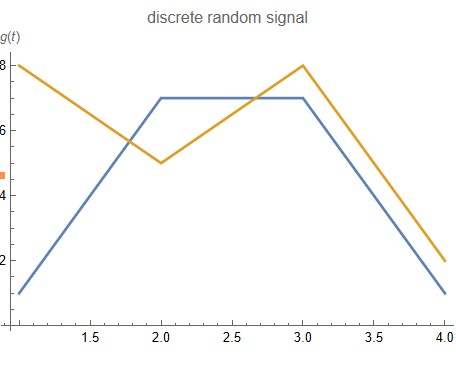
\includegraphics[width=7cm]{images/covariance.jpg}
 \caption{Covariance}
 \label{fig:signal values}
\end{figure}
$$
\begin{aligned}
& x=\{1,7,7,1\} \\
& y=\{8,5,8,2\} \\
& \bar{x} \quad=\frac{1}{N} \sum_{i=1}^N x_i \quad=4.0000 \\
& \bar{y}=\frac{1}{N} \sum_{i=1}^N y_i \quad=5.7500 \\
& \overline{x y}=\frac{1}{N} \sum_{i=1}^N x_i y_i \quad=25.2500 \\
& \hat{\sigma}_x=\sqrt{\frac{1}{N-1} \sum_{i=1}^N\left(x_i-\bar{x}\right)^2}=3.4641 \\
& \hat{\sigma}_y=\sqrt{\frac{1}{N-1} \sum_{i=1}^N\left(y_i-\bar{y}\right)^2}=2.8723 \\
& \hat{\sigma}_{x y}=\frac{\sum_{i=1}^n\left(X_i-\bar{X}\right)\left(Y_i-\bar{Y}\right)}{n-1}=3.0000 \\
& \hat{\rho}=\frac{\hat{\sigma}_{x y}}{\hat{\sigma}_x \hat{\sigma}_y}={0.3015} \\
&
\end{aligned}
$$
\subsubsection{Calculations}
To calculate the next sample in a kalman filter one must know what the following variables mean: 
\begin{itemize}
  \item $\mathbf{F}_k$, the state-transition model;
  \item $\mathbf{H}_k$, the observation model;
  \item $\mathbf{Q}_k$, the covariance of the process noise;
  \item $\mathbf{R}_k$ the covariance of the observation noise;
\end{itemize}



Furthermore one must be familiar with the \href{https://en.wikipedia.org/wiki/State-space_representation}{state space reperesentation}. Thereby the following \href{https://youtu.be/-cD7WkbAIL0}{video series} is very helpful.
For a Kalman-Filter one can use the following recipe:
\begin{enumerate}
  \item Set $k=0$, enter the prior estimate $\hat{\boldsymbol{x}}_{0 \mid-1}$ and an intial value for the erro covariance matrix $\boldsymbol{P}_{0 \mid-1}$
  \item Compute the Kalman gain: $\boldsymbol{k}_k=\boldsymbol{P}_{k \mid k-1} C^T\left(\boldsymbol{C} \boldsymbol{P}_{k \mid k-1} C^T+R_k\right)^{-1}$
  \item Update the estimate with the new measurement $y_k: \hat{\boldsymbol{x}}_{k \mid k}=\hat{\boldsymbol{x}}_{k \mid k-1}+\boldsymbol{k}_k\left(y_k-\boldsymbol{C} \hat{\boldsymbol{x}}_{k \mid k-1}\right)$
  \item Compute the error covariance matrix: $\boldsymbol{P}_{k \mid k}=\left(\boldsymbol{I}-\boldsymbol{k}_k \boldsymbol{C}\right) \boldsymbol{P}_{k \mid k-1}$
  \item Project ahed: $\hat{\boldsymbol{x}}_{k+1 \mid k}=\boldsymbol{A} \hat{\boldsymbol{x}}_{k \mid k}$ and $\boldsymbol{P}_{k+1 \mid k}=\boldsymbol{A} \boldsymbol{P}_{k \mid k} \boldsymbol{A}^T+\boldsymbol{Q}_k$
  \item Increment $k$ and return to step 2.
\end{enumerate}

\begin{equation}\label{eq:kalman_P_kk}
\begin{aligned}
\boldsymbol{P}_{k \mid k} &=E\left\{\left(\boldsymbol{x}_k-\hat{\boldsymbol{x}}_{k \mid k-1}\right)\left(\boldsymbol{x}_k-\hat{\boldsymbol{x}}_{k \mid k-1}\right)^T-\boldsymbol{k}_k e_{k \mid k-1}\left(\boldsymbol{x}_k-\hat{\boldsymbol{x}}_{k \mid k-1}\right)^T\right\} \\
&=\boldsymbol{P}_{k \mid k-1}-\boldsymbol{k}_k \boldsymbol{C} \boldsymbol{P}_{k \mid k-1} \\
&=\left(\boldsymbol{I}-\boldsymbol{k}_k \boldsymbol{C}\right) \boldsymbol{P}_{k \mid k-1} .
\end{aligned}
\end{equation}
\begin{equation}\label{eq:kalman_k_k}
k_k=\boldsymbol{P}_{k \mid k-1} C^T\left(C P_{k \mid k-1} C^T+R_k\right)^{-1}
\end{equation}
\begin{equation}\label{eq:kalman_x_kk}
\hat{\boldsymbol{x}}_{k \mid k}=\hat{\boldsymbol{x}}_{k \mid k-1}+\boldsymbol{k}_k\left(y_k-\boldsymbol{C} \hat{\boldsymbol{x}}_{k \mid k-1}\right)
\end{equation}
\begin{equation}\label{eq:kalman_P_kk+1}
\begin{aligned}
\boldsymbol{P}_{k+1 \mid k} &=E\left\{\left(\boldsymbol{x}_{k+1}-\hat{\boldsymbol{x}}_{k+1 \mid k}\right)\left(\boldsymbol{x}_{k+1}-\hat{\boldsymbol{x}}_{k+1 \mid k}\right)^T\right\} \\
&=E\left\{\boldsymbol{A}\left(\boldsymbol{x}_k-\hat{\boldsymbol{x}}_{k \mid k}\right)\left(\boldsymbol{x}_k-\hat{\boldsymbol{x}}_{k \mid k}\right)^T \boldsymbol{A}^T+\boldsymbol{u}_k \boldsymbol{u}_k^T\right\} \\
&=\boldsymbol{A} \boldsymbol{P}_{k \mid k} \boldsymbol{A}^T+\boldsymbol{Q}_k
\end{aligned}
\end{equation}
\begin{equation}\label{eq:kalman_x_kk_2}
\hat{\boldsymbol{x}}_{k \mid k}=\hat{\boldsymbol{x}}_{k \mid k-1}+\frac{\boldsymbol{P}_{k \mid k-1} \boldsymbol{C}^T}{\boldsymbol{C P _ { k | k - 1 } C ^ { T } + 1}}\left(y_k-\boldsymbol{C} \hat{\boldsymbol{x}}_{k \mid k-1}\right)
\end{equation}
\begin{equation}\label{eq:kalman_x_kk+1}
\boldsymbol{x}_{k+1}=\boldsymbol{A} \boldsymbol{x}_k+\boldsymbol{B} \boldsymbol{u}_k
\end{equation}






\begin{figure}[ht]
 \centering
 %\includestandalone[width=1\linewidth]{kalman.tex} % without the `.tex` extension
 \resizebox{1\textwidth}{!}{\subimport{images/}{kalman.tex}}
 \caption{Kalman example}
 \label{fig:kalman_1}
\end{figure}

\subsubsection{Example Kalman filter}
You are given a linear, shift-invariant system as depicted above. This system has the scalar state $x_k$ and produces
the scalar output $y_k$ at every discrete time instant $k$. The measurement-noise $v_k$ and the process-noise $u_k$ are zero-mean Gaussian random variables with $\textcolor{pink}{R_k} = E\{v_k^2\}=\textcolor{pink}{1}$ and $Q_k = E\{u_k^2\}= 1$.
\begin{figure}[ht]
 \centering
 %\includestandalone[width=1\linewidth]{kalman_example.tex} % without the `.tex` extension
 \resizebox{1\textwidth}{!}{\subimport{images/}{kalman_example.tex}}
 \caption{Kalman example}
 \label{fig:kalman_example}
\end{figure}


$$
\begin{array}{|c|c|c|c|}
\hline k & P_{k \mid k-1} & k_k & P_{k \mid k} \\
\hline 0 & \textcolor{blue}{\frac{4}{3}} & & \\
1 & & & \\
2 & & & \\
\hline
\end{array}
$$

$$
\begin{array}{|r|r|r|r|}
\hline k & y_k & \hat{x}_{k \mid k-1} & \hat{x}_{k \mid k} \\
\hline 0 & \textcolor{orange}{0.80} & \textcolor{brown}{0.00} & \\
1 & -1.20 & & \\
2 & 0.10 & & \\
\hline
\end{array}
$$

$$
\begin{array}{|c|c|c|c|}
\hline k & P_{k \mid k-1} & k_k & P_{k \mid k} \\
\hline 0 & 0 & & \\
1 & & & \\
2 & & & \\
\hline
\end{array}
$$

First one has to calculate $k_k$ which can be done with \autoref{eq:kalman_k_k}. From \autoref{fig:kalman_1} we know that $C=1$, $\textcolor{blue}{P_{k \mid k-1}}=\textcolor{blue}{\frac{4}{3}}$ and $R_k=1$. Therefore
$$
\textcolor{violet}{\boldsymbol{k}_k}=\textcolor{blue}{\boldsymbol{P}_{k \mid k-1}} C^T\left(\boldsymbol{C} \textcolor{blue}{\boldsymbol{P}_{k \mid k-1}} C^T+\textcolor{pink}{R_k}\right)^{-1}=\textcolor{blue}{\frac{4}{3}} \cdot 1 \cdot \left(1\cdot \textcolor{blue}{\frac{4}{3}}\cdot 1 +\textcolor{pink}{1} \right)^{-1}=\textcolor{violet}{\frac{4}{7}}
$$
In the next step one can calculate $\hat{x}_{k \mid k}$ with the new measurement $y_k$, therefore and due to \autoref{eq:kalman_x_kk}
$$
\textcolor{olive}{\hat{\boldsymbol{x}}_{k \mid k}}=\textcolor{brown}{\hat{\boldsymbol{x}}_{k \mid k-1}}+\textcolor{violet}{\boldsymbol{k}_k}\left(y_k-\boldsymbol{C} \hat{\boldsymbol{x}}_{k \mid k-1}\right)=\textcolor{brown}{0}+\textcolor{violet}{\frac{4}{7}}\cdot \left(\textcolor{orange}{\frac{4}{5}} - 1 \cdot \textcolor{brown}{0} \right)=\textcolor{olive}{\frac{16}{35}}
$$
With \autoref{eq:kalman_P_kk} one can now calculate $P_{k \mid k}$.
$$
\textcolor{teal}{\boldsymbol{P}_{k \mid k}}=\left(\boldsymbol{I}-\textcolor{violet}{\boldsymbol{k}_k} \boldsymbol{C}\right) \textcolor{blue}{\boldsymbol{P}_{k \mid k-1}}=\left(1-\textcolor{violet}{\frac{4}{7}}\cdot 1 \right) \cdot \textcolor{blue}{\frac{4}{3}}=\textcolor{teal}{\frac{4}{7}}
$$
In the next step, one can calculate $\textcolor{magenta}{\boldsymbol{P}_{k+1 \mid k}}$ with \autoref{eq:kalman_P_kk+1}
$$
\textcolor{magenta}{\boldsymbol{P}_{k+1 \mid k}}=\textcolor{red}{\boldsymbol{A}} \textcolor{teal}{\boldsymbol{P}_{k \mid k}} \textcolor{red}{\boldsymbol{A}}^T+\boldsymbol{Q}_k=\textcolor{red}{\frac{1}{2}}\cdot \textcolor{teal}{\frac{4}{7}} \cdot \textcolor{red}{\frac{1}{2}} +1=\textcolor{magenta}{\frac{8}{7}}
$$
With \autoref{eq:kalman_x_kk+1} one can calculate $\boldsymbol{x}_{k+1}$
$$
\hat{\boldsymbol{x}}_{k+1 \mid k}=\textcolor{red}{\boldsymbol{A}} \textcolor{olive}{\hat{\boldsymbol{x}}_{k \mid k}}=\textcolor{red}{\frac{1}{2}}\cdot \textcolor{olive}{\frac{16}{35}}=\frac{8}{35}
$$
Now one can repeat the steps before and one gets the following result:
$$
\begin{array}{|c|c|c|c|}
\hline k & P_{k \mid k-1} & k_k & P_{k \mid k} \\
\hline 0 & \textcolor{blue}{\frac{4}{3}} & \textcolor{violet}{\frac{4}{7}} & \textcolor{teal}{\frac{4}{7}} \\
1 & \textcolor{magenta}{\frac{8}{7}} & \frac{8}{15} & \frac{8}{15} \\
2 & \frac{17}{15} & \frac{17}{32} & \frac{17}{32} \\
\hline
\end{array}
$$




Now one can repeat the steps before and one gets the following result:

$$
\begin{array}{|r|r|r|r|}
\hline k & y_k & \hat{x}_{k \mid k-1} & \hat{x}_{k \mid k} \\
\hline 0 & \textcolor{orange}{0.80} & \textcolor{brown}{0.00} & \textcolor{olive}{\frac{16}{35}} \\
1 & -1.20 & \frac{8}{35} & -0.53 \\
2 & 0.10 & -0.27 & -0.07 \\
\hline
\end{array}
$$

$$
\begin{array}{|c|c|c|c|}
\hline k & P_{k \mid k-1} & k_k & P_{k \mid k} \\
\hline 0 & 0 & 0 & 0 \\
1 & 1 & \frac{1}{2} & \frac{1}{2} \\
2 & \frac{9}{8} & \frac{9}{17} & \frac{9}{17} \\
\hline
\end{array}
$$
Alternatively, one can also program a \href{https://youtu.be/x0-NaGaCzew}{program} on the ti-nspire and call it then like the following:
\begin{verbatim}
sign_proc\kalman(1,1,((4)/(3)),0,[((1)/(2))],[1],[1],((4)/(5)))
\end{verbatim}
sign\_proc\textbackslash kalman($R_k$,$Q_k$,$P_{k|k-1}$,$x_{k|k-1}$,$A$,$B$,$C$,$y_k$)\newline
which outputs then the following:\newline
$R_k: 1 , Q_k: 1 , P_{k|k-1}: ((4)/(3)) , x_{k|k-1}: 0 , A: [((1)/(2))] , B: [1] , C: [1] , y_k: ((4)/(5))$
$k_k= [(\textcolor{violet}{(4)/(7)})] , \hat{x}_{k_k}= [(\textcolor{olive}{(16)/(35)})] , p_{k|k}= [(\textcolor{teal}{(4)/(7)})] , x_{k+1|k}= [((8)/(35))] , p_{k+1|k}= [(\textcolor{pink}{(8)/(7)})]$\newline
The program itself looks like the following:
\begin{verbatim}
Define LibPub kalman(r_k,q_k,pkk_m_1,xkk_m_1,a,b,c,y_k)=
Prgm
:©Inputs a(R_k (covariance of observation noise), R_k (covariance of the proccess noise), pkk_m_1,xkk_m_1, a,b,c,y_k)
:Disp "R_k: ",r_k,", Q_k: ",q_k,", P_{k|k-1}: ",pkk_m_1,", x_{k|k-1}: ",xkk_m_1," , A: ",a," , B: ",b," , C: ",c," , y_k: ",y_k
:Disp " "
:Local k_k,x_k_k,p_k_k,xkk_p_1,pkk_p_1
:k_k:=pkk_m_1*c^T*(c*pkk_m_1*c^T+r_k)^(-1)
:x_k_k:=xkk_m_1+k_k*(y_k-c*xkk_m_1)
:p_k_k:=(identity(max(dim(c)))-k_k*c)*pkk_m_1
:xkk_p_1:=a*x_k_k
:pkk_p_1:=a*p_k_k*a^T+q_k
:Disp "k_k=",k_k," , \hat{x}_{k_k}=",x_k_k," , p_{k|k}=",p_k_k," , x_{k+1|k}=",xkk_p_1," , p_{k+1|k}=",pkk_p_1
:PassErr
:EndPrgm
\end{verbatim}

\subsubsection{Example 2}
Lets assume we want to measure the position of an airplane, with $v_{0 x}=280$ and $x_0=4000\mathrm{~m}$.
\paragraph{Observations}
$$
\begin{array}{ll}
x_0=4000 \mathrm{~m} & v_{0 x}=280 \mathrm{~m} / \mathrm{sec} \\
x_1=4260 \mathrm{~m} & v_{1 x}=282 \mathrm{~m} / \mathrm{sec} \\
x_2=4550 \mathrm{~m} & v_{2 x}=285 \mathrm{~m} / \mathrm{sec} \\
x_3=4860 \mathrm{~m} & v_{3 x}=286 \mathrm{~m} / \mathrm{ser} \\
x_4=5110 \mathrm{~m} & v_{4 x}=290 \mathrm{~m} / \mathrm{sec}
\end{array}
$$
\paragraph{Initial Conditions}
$$
\begin{array}{ll}
a_x=2 \mathrm{~m} / \mathrm{sec}^2 & \Delta t=1 \mathrm{sec} \\
V_x=280 \mathrm{~m} / \mathrm{sec} & \Delta x=25 \mathrm{~m}
\end{array}
$$
\paragraph{Process Errors i Process covariance matrix}
$$
\begin{aligned}
&\Delta P_x=20 \mathrm{~m} \\
&\Delta P_{v_x}=5 \mathrm{~m} / \mathrm{sec}
\end{aligned}
$$
\paragraph{Observations errors}
$$
\begin{aligned}
&\Delta x=25 \mathrm{~m} \\
&\Delta v_x=6 \mathrm{~m} / \mathrm{sec}
\end{aligned}
$$
Our estimate of $X_{k_p}$ which is the next state is the following:
$$
\begin{aligned}
X_{k_p} &=A X_{k-1}+B u_k+w_k \\
&=\left[\begin{array}{ll}
1 & \Delta t \\
0 & 1
\end{array}\right]\left[\begin{array}{c}
x_0 \\
v_0
\end{array}\right]+\left[\begin{array}{c}
\frac{1}{2} \Delta t^2 \\
\Delta t
\end{array}\right]\left[a_{x_0}\right]+0 \\
&=\left[\begin{array}{ll}
1 & 1 \\
0 & 1
\end{array}\right]\left[\begin{array}{c}
4000 \\
280
\end{array}\right]+\left[\begin{array}{c}
1 / 2 \\
1
\end{array}\right]\left[\begin{array}{l}
2
\end{array}\right] \\
&=\left[\begin{array}{c}
4280 \\
280
\end{array}\right]+\left[\begin{array}{l}
1 \\
2
\end{array}\right] \\
X_{k_p} &=\left[\begin{array}{c}
4281 \\
282
\end{array}\right]
\end{aligned}
$$
\paragraph{Initial Process Covariance}
The cross term is often set to zero, since they are independent of each other.
$$
\begin{aligned}
&P_{k-1}=\left[\begin{array}{cc}
\Delta x^2 & \Delta x \Delta v \\
\Delta x \Delta v & \Delta v_x^2
\end{array}\right]=\left[\begin{array}{ll}
400 & 100 \\
100 & 25
\end{array}\right] \\
&P_{k-1}=\left[\begin{array}{cc}
400 & 0 \\
0 & 25
\end{array}\right]
\end{aligned}
$$
\paragraph{The predicted process covariance matrix}
$$
\begin{aligned}
P_{k p} &=A P_{k-1} A^{\top}+Q_R \\
&=\left[\begin{array}{ll}
1 & \Delta t \\
0 & 1
\end{array}\right]\left[\begin{array}{cc}
400 & 0 \\
0 & 25
\end{array}\right]\left[\begin{array}{ll}
1 & 0 \\
\Delta t & 1
\end{array}\right]+0 \\
&=\left[\begin{array}{ll}
1 & 1 \\
0 & 1
\end{array}\right]\left[\begin{array}{cc}
400 & 0 \\
0 & 25
\end{array}\right]\left[\begin{array}{ll}
1 & 0 \\
1 & 1
\end{array}\right] \\
&=\left[\begin{array}{cc}
400 & 25 \\
0 & 25
\end{array}\right]\left[\begin{array}{ll}
1 & 0 \\
1 & 1
\end{array}\right] \\
&=\left[\begin{array}{ll}
425 & 25 \\
25 & 25
\end{array}\right] \Rightarrow\left[\begin{array}{cc}
425 & 0 \\
0 & 25
\end{array}\right]
\end{aligned}
$$
\paragraph{Calculating the Calman Gain}
$$
\begin{aligned}
K &=\frac{P_{k_p} H^{\top}}{H P_{k_p} H^{\top}+R} \\
&=\frac{\left[\begin{array}{cc}
425 & 0 \\
0 & 25
\end{array}\right]\left[\begin{array}{ll}
1 & 0 \\
0 & 1
\end{array}\right]}{\left[\begin{array}{ll}
1 & 0 \\
0 & 1
\end{array}\right]\left[\begin{array}{cc}
425 & 0 \\
0 & 25
\end{array}\right]\left[\begin{array}{ll}
1 & 0 \\
0 & 1
\end{array}\right]+\left[\begin{array}{cc}
625 & 0 \\
0 & 36
\end{array}\right]} \\
&=\frac{\left[\begin{array}{cc}
425 & 0 \\
0 & 25
\end{array}\right]}{\left[\begin{array}{cc}
425 & 0 \\
0 & 25
\end{array}\right]+\left[\begin{array}{cc}
625 & 0 \\
0 & 36
\end{array}\right]}=\frac{\left[\begin{array}{cc}
425 & 0 \\
0 & 25
\end{array}\right]}{\left[\begin{array}{cc}
1050 & 0 \\
0 & 61
\end{array}\right]}=\left[\begin{array}{cc}
0.405 & 0 \\
0 & 0.410
\end{array}\right]
\end{aligned}
$$
\paragraph{The new Observation}
$$
\begin{aligned}
&Y_k=C y_k+Z_k \\
&Y_k=\left[\begin{array}{ll}
1 & 0 \\
0 & 1
\end{array}\right]\left[\begin{array}{c}
4260 \\
282
\end{array}\right]+0 \\
&Y_k=\left[\begin{array}{l}
4260 \\
282
\end{array}\right]
\end{aligned}
$$
\paragraph{Calculate the current state}
$$
\begin{aligned}
&X_k=X_{k_p}+K\left[Y_k-H X_{k_p}\right]\\
&=\left[\begin{array}{l}
4281 \\
282
\end{array}\right]+\left[\begin{array}{cc}
0.405 & 0 \\
0 & 0.410
\end{array}\right]\left(\left[\begin{array}{l}
4260 \\
282
\end{array}\right]-\left[\begin{array}{cc}
1 & 0 \\
0 & 1
\end{array}\right]\left[\begin{array}{ll}
4281 \\
282
\end{array}\right]\right)\\
&=\left[\begin{array}{c}
4281 \\
282
\end{array}\right]+\left[\begin{array}{cc}
0.405 & 0 \\
0 & 0.410
\end{array}\right]\left[\begin{array}{c}
-21 \\
0
\end{array}\right]\\
&=\left[\begin{array}{c}
4281 \\
282
\end{array}\right]+\left[\begin{array}{c}
-8.5 \\
0
\end{array}\right]\\
&X_k=\left[\begin{array}{c}
4272.5 \\
282
\end{array}\right]
\end{aligned}
$$
\paragraph{Update Process Covariance}
$$
\begin{aligned}
&P_k=(I-K H) P_{k_p}\\
&P_k=\left[\left[\begin{array}{ll}
1 & 0 \\
0 & 1
\end{array}\right]-\left[\begin{array}{cc}
0.405 & 0 \\
0 & 0.410
\end{array}\right]\left[\begin{array}{ll}
1 & 0 \\
0 & 1
\end{array}\right]\left[\begin{array}{cc}
425 & 0 \\
0 & 25
\end{array}\right]\right.\\
&P_k=\left[\left[\begin{array}{ll}
1 & 0 \\
0 & 1
\end{array}\right]-\left[\begin{array}{cc}
0.405 & 0 \\
0 & 0.410
\end{array}\right]\left[\begin{array}{cc}
425 & 0 \\
0 & 25
\end{array}\right]\right.\\
&k=\left[\begin{array}{cc}
0.595 & 0 \\
0 & 0.590
\end{array}\right]\left[\begin{array}{cc}
425 & 0 \\
0 & 25
\end{array}\right]\\
&P_k=\left[\begin{array}{cc}
253 & 0 \\
0 & 14.8
\end{array}\right]
\end{aligned}
$$
\paragraph{Current Becomes previous}
$$
\begin{aligned}
&X_k=\left[\begin{array}{c}
4272.5 \\
282
\end{array}\right] \Rightarrow X_{k-1} \Rightarrow X_{k_p}=A X_{k-1}+B_k+w_k \\
&P_k=\left[\begin{array}{cc}
253 & 0 \\
0 & 14.8
\end{array}\right] \Rightarrow P_{k-1} \Rightarrow P_{k_p}=A P_{k-1} A^{\top}+Q_k
\end{aligned}
$$
\section{CDMA (code division multiple access)}
The idea behind this system is that all transmitters use the same time and frequency allocation. To distinguish the different users, a code is assigned to each of them. The code is then used to spread a small information bandwidth over the much wider channel bandwidth. CDMA is thus a spread spectrum (FH-SS) technique. There are two ways to do that, one is frequency hopping (FH-SS) and the other is by  multiplying the data sequence with a much higher chip sequence (DSSS), as one can see in \autoref{fig:dsss}.
\begin{figure}[ht]
  \centering
  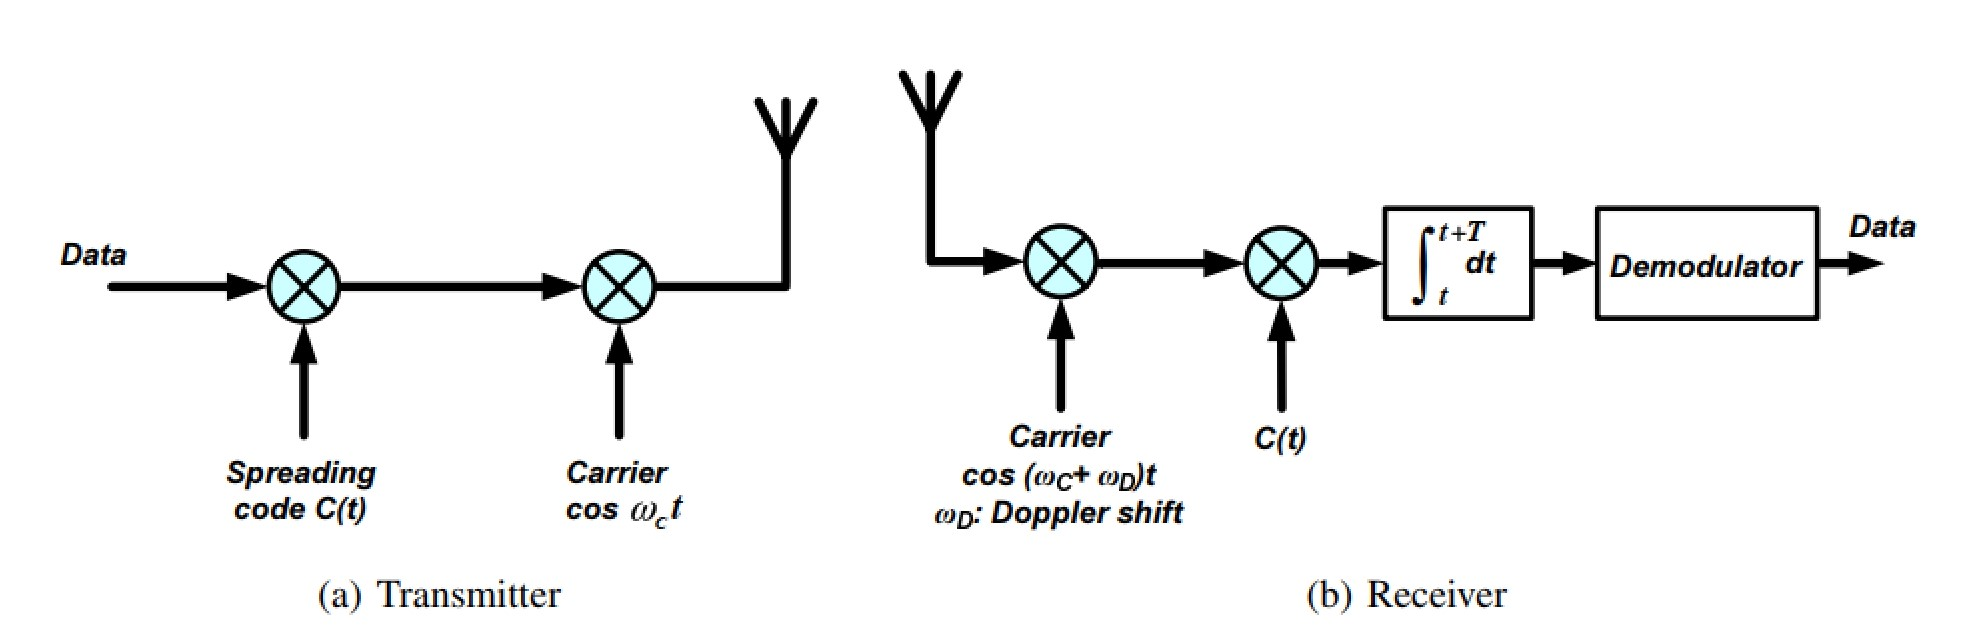
\includegraphics[width=13cm]{images/spread_spectrum_tx_rx.jpg}
  \caption{Spread Sepctrum}
  \label{fig:dsss}
\end{figure}
The spreading gain of such a system can be calculated according to \autoref{eq:spreading_gain}, where the bit time is called $T_d$ and the chip time $T_c$.
\begin{equation}\label{eq:spreading_gain}
G_{\mathrm{dB}}=10 \log _{10} \frac{\mathrm{SNR}_{\text {out }}}{\mathrm{SNR}_{\text {in }}}=10 \log _{10} \frac{B_{\mathrm{ss}}}{B_{\mathrm{d}}}=10 \log _{10} \frac{T_{\mathrm{d}}}{T_{\mathrm{c}}}
\end{equation}
\subsubsection{Shor Summary}
CDMA (Code Division Multiple Access) is a wireless communication technology that uses unique codes to separate different signals in the same frequency band. It was mainly used in some areas for 2G and 3G cellular network technology.

Spreading is the process of assigning a unique code to each user's data to distinguish it from other users' data. The receiver then applies the same code to decode the intended data (For that one uses the m-sequences (Glonass), Gold codes (e.g. GPS)). Spreading allows multiple users to share the same frequency band simultaneously by separating their signals through code division. This results in an increase in the number of users that can access the network and improves the overall network capacity. (When doing this, one increases the bandwidth (frequency))
\subsection{UMTS (Universal Mobile Telecommunications System)}
Is the most prominent communication system in Europe. As opposed to GSM and other TDMA-based cellular systems, where one user has a link to one cell only at one given time, a UTMS user can use signals from two base stations. They send with the same user code, such that the signal looks as if it was sent through a multipath environment. Thus, we do not have a hard handover when changing from one cell to another, but rather a smooth, so-called soft handover, where the user may have a simultaneous link to two base stations during a transition phase
\subsection{Hadamard matrix / Walsh matrices}
Hadamard matrix / Walsh matrices are used to generate the code for the different users in a system as it can also be seen in \autoref{subsubsec:example_cdma}.
The equation to calculate the Hadamard matrix can be found in \autoref{eq:hadamard}. To do the calculation one must know the Kronecker Product ($\otimes$) to which an example can be found in \autoref{eq:kronecker_example}. An important property of the Hadamard matrix is that when one multiplies two rows with each other and ads them up the result is always zero see also \autoref{eq:hardamard_test}. In the end one multiplies the signal for a certain user with one column of the matrix. The receiver (user) does the same and is then able to decode the signal.
\begin{equation} \label{eq:hadamard}
\begin{aligned}
&H_1=[1],\\
&H_2=\left[\begin{array}{cc}
1 & 1 \\
1 & -1
\end{array}\right] \text {, }\\
&H_4=\left[\begin{array}{cccc}
1 & 1 & 1 & 1 \\
1 & -1 & 1 & -1 \\
1 & 1 & -1 & -1 \\
1 & -1 & -1 & 1
\end{array}\right]\\
&H_{2^k}=\left[\begin{array}{cc}
H_{2^{k-1}} & H_{2^{k-1}} \\
H_{2^{k-1}} & -H_{2^{k-1}}
\end{array}\right]=H_2 \otimes H_{2^{k-1}}
\end{aligned}
\end{equation}
\subsubsection{Kronecker Product}
\begin{equation}\label{eq:kronecker_example}
\left[\begin{array}{ll}
1 & 2 \\
3 & 4
\end{array}\right] \otimes\left[\begin{array}{ll}
0 & 5 \\
6 & 7
\end{array}\right]-\left[\begin{array}{llll}
1 \cdot 0 & 1 \cdot 5 & 2 \cdot 0 & 2 \cdot 5 \\
1 \cdot 6 & 1 \cdot 7 & 2 \cdot 6 & 2 \cdot 7 \\
3 \cdot 0 & 3 \cdot 5 & 4 \cdot 0 & 4 \cdot 5 \\
3 \cdot 6 & 3 \cdot 7 & 4 \cdot 6 & 4 \cdot 7
\end{array}\right]-\left[\begin{array}{cccc}
0 & 5 & 0 & 10 \\
6 & 7 & 12 & 14 \\
0 & 15 & 0 & 20 \\
18 & 21 & 24 & 28
\end{array}\right]
\end{equation}
\subsubsection{carrier-to-interference ratio (C/I)}
The carrier-to-interference ratio (C/I) in CDMA refers to the ratio of the power of the desired signal to the power of the unwanted interference in the system. A higher C/I ratio indicates a better signal quality and a lower level of interference, which can result in improved system performance and capacity. For example a carrier-to-interference ratio (C/I) of 1000 means that the power of the desired signal is 1000 times greater than the power of the unwanted interference. This indicates that the signal quality is very good and there is a low level of interference in the system. A high C/I ratio is desirable in CDMA communication systems as it results in improved system performance and capacity. A C/I ratio of 1000 is considered very high and provides excellent signal quality and minimal interference.
\subsubsection{Exercise calculate hadamard matrix}
Construct the Hadamard matrix $H_8$ and check the orthogonality property of the codes given by row 2 and row 8, respectively.
$$
H_8=\left[\begin{array}{cccccccc}
1 & 1 & 1 & 1 & 1 & 1 & 1 & 1 \\
1 & -1 & 1 & -1 & 1 & -1 & 1 & -1 \\
1 & 1 & -1 & -1 & 1 & 1 & -1 & -1 \\
1 & -1 & -1 & 1 & 1 & -1 & -1 & 1 \\
1 & 1 & 1 & 1 & -1 & -1 & -1 & -1 \\
1 & -1 & 1 & -1 & -1 & 1 & -1 & 1 \\
1 & 1 & -1 & -1 & -1 & -1 & 1 & 1 \\
1 & -1 & -1 & 1 & -1 & 1 & 1 & -1
\end{array}\right]
$$
\begin{equation}\label{eq:hardamard_test}
\begin{aligned}
H_{8_2} \cdot H_{8_8}^T & =\left[\begin{array}{llllllll}
1 & -1 & 1 & -1 & 1 & -1 & 1 & -1
\end{array}\right] \cdot\left[\begin{array}{llllllll}
1 & -1 & -1 & 1 & -1 & 1 & 1 & -1
\end{array}\right]^T \\
& =1+1-1-1-1-1+1+1=0 .
\end{aligned}
\end{equation}
\subsubsection{Exercise CDMA}
Now let us assume a CDMA system with a data rate of 125 kbit/s (BPSK with a $\pm $1 data stream), a chip rate of 1 Mchip/s and a carrier frequency of $f_c$. Sketch the transmitter of such a system and assign important parameters.
\paragraph{Sketch the receiver of such a system and assign important parameters.}\mbox{} \newline
See \autoref{fig:dsss}
\paragraph{Sketch the receiver of such a system and assign important parameters.}\mbox{} \newline
See \autoref{fig:dsss}
\paragraph{Draw in a qualitative way the amplitude spectrum around the RF carrier of the RF signal with only data modulated (no spreading).}\mbox{} \newline
Since the pulse duration is \SI{8e-6}{\second} and the Fourier transform of a rectangle is $|T| \cdot \operatorname{si}(\pi T f)=\SI{8e-6}{}\frac{sin(\SI{8e-6}{\second} \cdot \pi \cdot f)}{\pi \cdot \SI{8e-6}{\second}}$ one can draw the graph. Important to know is that when one solves the following equations$\frac{sin(\SI{8e-6}{\second} \cdot \pi \cdot f)}{\pi \cdot \SI{8e-6}{\second}}=0 \Rightarrow \SI{8e-6}{\second} \cdot \pi \cdot f=\pi$ one gets \SI{125e3}{\hertz} which is half of the null to null bandwidth $\Rightarrow$ the null to null bandwidth is \SI{250e3}{\hertz}, see \autoref{fig:amp_spec1}.
\begin{figure}[ht!]
  \centering
  \resizebox{12cm}{!}{\subimport{images/}{amplitude_spectrum_1.tex}}
  \caption{Amplitude Spectrum}
  \label{fig:amp_spec1}
\end{figure}
\paragraph{Draw in a qualitative way the amplitude spectrum around the RF carrier of the spread RF signal}\mbox{} \newline
Since the pulse duration is \SI{1e-6}{\second} and the Fourier transform of a rectangle is $|T| \cdot \operatorname{si}(\pi T f)=\SI{1e-6}{}\frac{sin(\SI{1e-6}{\second} \cdot \pi \cdot f)}{\pi \cdot \SI{1e-6}{\second}}$ one can draw the graph. Important to know is that when one solves the following equations$\frac{sin(\SI{1e-6}{\second} \cdot \pi \cdot f)}{\pi \cdot \SI{1e-6}{\second}}=0 \Rightarrow \SI{1e-6}{\second} \cdot \pi \cdot f=\pi$ one gets \SI{1e6}{\hertz} which is half of the null to null bandwidth $\Rightarrow$ the null to null bandwidth is \SI{2e6}{\hertz},see \autoref{fig:amp_spec2}.
\begin{figure}[ht!]
  \centering
  \resizebox{12cm}{!}{\subimport{images/}{amplitude_spectrum_2.tex}}
  \caption{Amplitude Spectrum}
  \label{fig:amp_spec2}
\end{figure}
\paragraph{What is the spreading gain}\mbox{} \newline
According to \autoref{eq:spreading_gain} it is $G_{\mathrm{dB}}=10 \log _{10} \frac{T_{\mathrm{d}}}{T_{\mathrm{c}}}=10 \log _{10} \frac{\SI{8e-6}{\second}}{\SI{1e-6}{\second}} \approx 9dB$. The spreading factor would be 8 since the frequency was increased by 8. But this also means the power density maximum has decreased by a factor of 9dB.
\subsubsection{Example 1} \label{subsubsec:example_cdma}
Walsh code should be used with a spreading factor of four and two users should use the channel at the same time. We know from \autoref{eq:hadamard} that with a spreading factor of four we get the following matrix\footnote{\href{https://youtu.be/L4Gvu3gQ0wg}{Video}}:
$$
H_4=\left[\begin{array}{cccc}
\rowcolor{red!20}
1 & 1 & 1 & 1 \\
\rowcolor{green!20}
1 & -1 & 1 & -1 \\
1 & 1 & -1 & -1 \\
1 & -1 & -1 & 1
\end{array}\right]\\
$$
One now has to assign to each user one code. Let's say \colorbox{red!20}{user one} has row one and \colorbox{green!20}{user two} row two. The other rows are inactive. \newline
Let's assume the Data of the users are the following: 
$$
\begin{array}{cccc}
\rowcolor{red!20}
\text{User}_1 & 110010 \\
\rowcolor{green!20}
\text{User}_2 & 001001
\end{array}
$$
This gives then the following \colorbox{blue!20}{code sequence}:\newline
\resizebox{1\textwidth}{!}{$\displaystyle
\begin{array}{llllllllllllllllllllllllll}
\rowcolor{red!20}
1&1&1&1&\mid1&1&1&1&\mid-1&-1&-1&-1&\mid-1&-1&-1&-1&\mid1&1&1&1& \mid-1&-1&-1&-1& \\
\rowcolor{green!20}
-1&1&-1&1&\mid-1&1&-1&1&\mid 1&-1&1&-1&\mid-1&1&-1&1&\mid-1&1&-1&1& \mid 1&-1&1&-1& \\
\rowcolor{blue!20}
0&2&0&2&\mid0&2&0&2&\mid0&-2&0&-2&\mid-2&0&-2&0&\mid0&2&0&2&\mid 0&-2&0&-2&
\end{array}
$}
The receiver does then a sequence wise multiplication with the received data and the assigned walsh-code, which is for user one 1111.\newline
\resizebox{1\textwidth}{!}{$\displaystyle
\begin{array}{llllllllllllllllllllllllll}
\rowcolor{blue!20}
0&2&0&2&\mid0&2&0&2&\mid0&-2&0&-2&\mid-2&0&-2&0&\mid0&2&0&2&\mid 0&-2&0&-2&\\
\rowcolor{red!20}
&&4&&\mid&&4&&\mid&&-4&&\mid&&-4&&\mid&&4&& \mid&&-4&& \\
\end{array}
$}
As one can see from the result above one gets the exact same data as one has transmitted.
\subsection{Frequency hopping}
We do frequency hopping so that if we have interference on a certain frequency, for example from a microwave, one can still receive and send data some data and not all is lost, but only some. To do this the transmitter and receiver are hopping in the same rhythm from one frequency to the other. Fast FHSS (Frequency hopping spread spectrum) means that one bit gets transmitted over multiple frequencies is not used, because one would need to switch the frequency very fast. Slow FHSS each bit gets transmitted over one frequency $\Rightarrow$ Hamming can be used to reconstruct false ones.

\paragraph{What is spreading gain?}\mbox{} \newline
See \autoref{eq:spreading_gain}
\paragraph{What is cell breathing?}\mbox{} \newline
In CDMA-based Cellular networks, cell breathing is a mechanism which allows overloaded cells to offload subscriber traffic to neighbouring cells by changing the geographic size of their service area. Heavily loaded cells decrease in size while neighbouring cells increase their service area to compensate. Thus, some traffic is handed off from the overloaded cell to neighbouring cells, resulting in load balancing.
\subsubsection{Excercise SNR vs. C/I in a CDMA system}
The signal-to-noise ratio given by thermal noise is usually designated as SNR. The corresponding signal-tonoise ratio due to interference by other users on the same channel is described by C/I (carrier-to-interference ratio).\newline
Now consider the following situation. A certain CDMA system can live with an SNR of 10 dB, if no additional
interference is present.
\begin{enumerate}
    \item \textbf{How much would you have to amplify the transmitter power in order to reach an SNR of 13 dB?}\newline
    By a factor of two, because 3db ($10^{\frac{3}{10}}=2$).
    \item \textbf{If spreading codes can be chosen such that a concurrent transmitter produces a C/I of 1000/1, how many transmitters can transmit simultaneously if the total signal-to-noise-plus-interference-ratio SINR is not to fall below the original 10 dB? The SINR is given by the linear measure}
    $$
    \frac{1}{\mathrm{SINR}}=\frac{1}{\mathrm{SNR}}+\frac{1}{C / I}
    $$
    SINR stands for Signal-to-Interference-plus-Noise Ratio in CDMA. It is a measure of the quality of a received signal compared to the combined power of all other interference signals and background noise. A high SINR indicates a strong signal and low interference and noise, while a low SINR indicates weak signal quality and high levels of interference and noise. SINR is an important performance metric in CDMA communication systems as it directly impacts the ability to accurately recover the intended signal. A high SINR results in improved system performance and capacity, while a low SINR can lead to errors and degradation of system performance.
    \item  \textbf{Can you allow more simultaneous transmitters for the same SINR by increasing all transmitter powers?
    $$
    \begin{aligned}
    \frac{1}{\frac{S}{I+N}}=\frac{1}{\text { SINR }} & =\frac{1}{\mathrm{SNR}}+\frac{1}{C / I} \\
    \frac{1}{10} & =\frac{1}{20}+\frac{1}{20} \\
    C / I & =13 \mathrm{~dB}=20 \\
    n \cdot \frac{1}{1000} & =\frac{1}{20} \Rightarrow n=\underline{50}
    \end{aligned}
    $$
Where are the limits?}\newline
\end{enumerate}
\subsection{M-Sequences}
Maximum-length sequences have very interesting autocorrelation properties: they have one peak for exact alignment, and the same low level for misalignment of one or more chips.
\begin{equation}
\begin{array}{ccc}
\hline \text { Degree }(L) & \text { Sequence length }\left(N=2^L-1\right) & \text { Primitive polynomial } \\
\hline 1 & 1 & x+1 \\
2 & 3 & x^2+x+1 \\
3 & 7 & x^3+x+1 \\
4 & 15 & x^4+x+1 \\
5 & 31 & x^5+x^2+1 \\
6 & 63 & x^6+x+1 \\
7 & 127 & x^7+x+1 \\
8 & 255 & x^8+x^7+x^2+x+1 \\
9 & 511 & x^9+x^4+1 \\
10 & 1023 & x^{10}+x^3+1 \\
11 & 2047 & x^{11}+x^2+1 \\
12 & 4095 & x^{12}+x^6+x^4+x+1 \\
\hline
\end{array}
\end{equation}
\begin{figure}[ht]
  \centering
  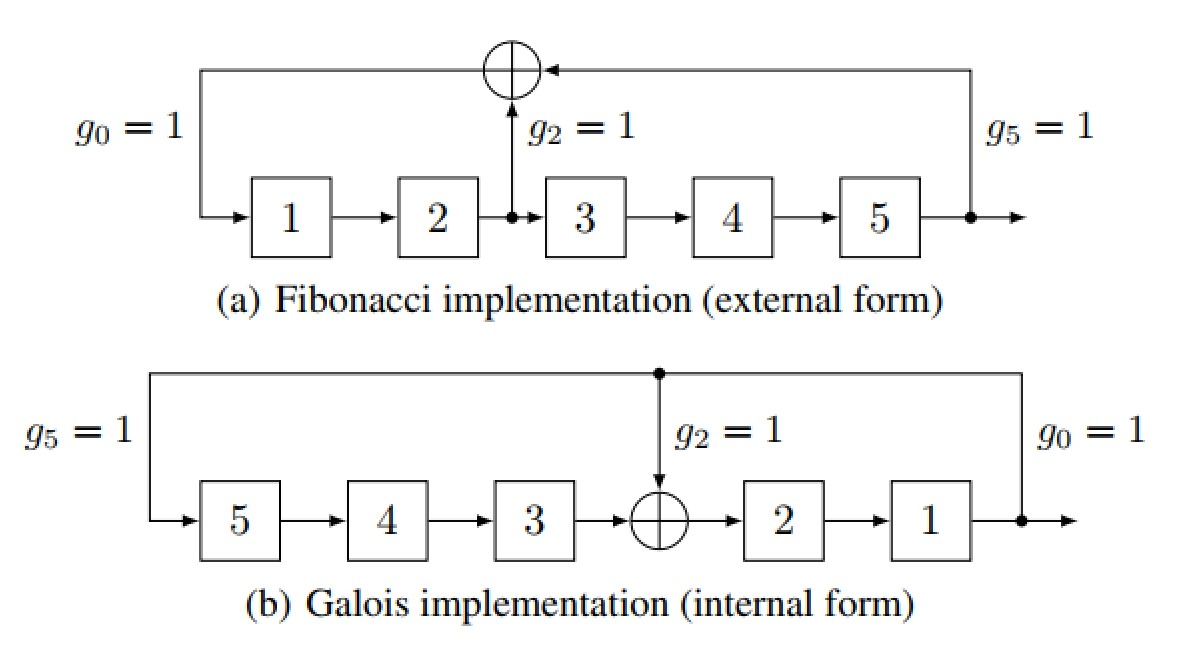
\includegraphics[width=13cm]{images/m-squences.jpg}
  \caption{Example of equivalent forms corresponding to a feedback polynomial of $x^5+x^2+1$.}
  \label{fig:m-squences}
\end{figure}
\subsection{UWB}
A signal is consider as ultra wide band when $\nu$ from \autoref{eq:uwb_condition} is larger than 20\%
\begin{equation}\label{eq:uwb_condition}
\nu=\frac{f_h-f_l}{f_c}=2 \frac{f_h-f_l}{f_h+f_l}
\end{equation}
\begin{itemize}
    \item $f_h$: higher cut off frequency
    \item $f_l$: lower cut off frequency
    \item $f_c$: center frequency
\end{itemize}

\section{OFDM}
OFDM has the benefit that frequency-selective fading is no problem and no spectrum is wasted for guard bands. Nevertheless, guard intervals are inserted to prevent ICI(inter channel interference) The following \href{https://youtu.be/i3LBGw8Yle4}{video} might be helpful.
The equalizer is in the frequency domain, and therefore it is much easier.\newline
The total excess delay is the total difference from the first and last signal received through the channel due to reflection. The mean delay of a received signal can be calculated according to \autoref{eq:mean_delay}, where $P_T$ is the power of the transmitted signal and can be calculated according to \autoref{eq:signal_power}. The delay spread can be calculated according to \autoref{eq:rms_delay_spread} and is dependent on \autoref{eq:signal_power} and \autoref{eq:mean_delay}. The delay spread has quite an important role in OFDM, since it defines the guard intervals.
\begin{equation}\label{eq:mean_delay}
\tau_0=\frac{1}{P_T} \sum_k P_k \tau_k
\end{equation}
\begin{equation}\label{eq:rms_delay_spread}
\begin{aligned}
\tau_{\mathrm{RMS}} =\sqrt{\frac{1}{P_T} \sum_k P_k\left(\tau_k-\tau_0\right)^2}
\end{aligned}
\end{equation}
\begin{equation}\label{eq:signal_power}
P_T =\sum_k P_k
\end{equation}
\subsubsection{Exercise Channel Impulse response and Coherence time/bandwidth}
\begin{enumerate}
    \item \textbf{What is the mean delay of a channel with the impulse response of $h(t)=\delta(t)+0.5 \delta\left(t-T_1\right)$ and $T_1=1\mu s$?}
    $$
    \tau_0=\frac{1}{1.25}\left(1^2\cdot \SI{0}{\micro\second}+0.5^2 \cdot \SI{1}{\micro\second}\right)=0.2 \mu \mathrm{s}
    $$
    \item \textbf{What is the spread of the signal mentioned above?}
    $$
    \tau_{\mathrm{RMS}}=\sqrt{\frac{1}{1.25}\left(1^2\cdot(0-0.2)^2+0.5^2 \cdot(1-0.2)^2\right)}=0.4 \mu \mathrm{s}
    $$
    \item \textbf{How does the impulse response look like?}\newline
    (two Dirac pulses, one delayed by T1 and attenuated to half the first one)
    \item \textbf{How would a possible environment look like?} \newline
    \SI{1}{\micro\second} corresponds to around \SI{300}{\meter}, There fore one has a direct path and a object that has a distanc that the signal must travel 300m more than in the direct path.
    \item \textbf{How would the frequency response look like obtained in the Fourier domain?}
    $$
    H(f)=1+0.5 \exp \left(-j 2 \pi f T_1\right)
    $$
    \item\textbf{ Draw the spectrum:}
    \begin{figure}[ht]
        \centering
        \includegraphics[width=13cm]{images/amplitude_spectrum_5.tex}
        \caption{Amplitude Spectrum}
        \label{fig:amp_spec_5}
    \end{figure}
    \begin{figure}[ht]
        \centering
        \includegraphics[width=13cm]{images/amplitude_spectrum_6.tex}
        \caption{Amplitude Spectrum}
        \label{fig:amp_spec_5}
    \end{figure}
    \FloatBarrier
    \item \textbf{Estimate the coherence bandwidth of this channel from the graph sketched} \newline
    Less than 100kHz (smallest bandwidth where the signal changes by 3dB)
    \item \textbf{Compute the coherence bandwidth of this channel and compare it with your estimated value:}\newline
    Depending on the definition we either have
    $$
    B_{\mathrm{coh}}=\frac{1}{2 \pi \tau_{\mathrm{RMS}}}=\frac{1}{2 \pi \cdot 0.4 \mu \mathrm{s}}=398 \mathrm{kHz}
    $$
    or, if the correlation function (among the impulse response at the different frequency positions) is to be $>0.9$
    $$
    B_{\mathrm{coh}}=\frac{1}{50 \tau_{\mathrm{RMS}}}=\frac{1}{50 \cdot 0.4 \mu \mathrm{s}}=50 \mathrm{kHz}
    $$
    \item \textbf{What is the coherence time of this channel?} \newline
    $\infty$, since nothing is moving, environment does not change.
    
\end{enumerate}
\subsubsection{Exercise Coherence time/Coherence Bandwidth}
Given is a wirless system with the following parameters:
\begin{itemize}
    \item Bandwidth w: 20MHz
    \item $f_{RF}$ = \SI{5}{\giga\hertz}
    \item Subcarrier spacing $\Delta f$ = \SI{312.5}{\kilo\hertz}
    \item Symbol time = \SI{3.2}{\micro\second}
    \item Guard interval = \SI{0.8}{\micro\second}
\end{itemize}
\begin{enumerate}
    \item \textbf{Is the coherence time of the channel long enough?} \newline
    From \autoref{eq:ofdm_rule_of_thumb4} and \autoref{eq:doppler_spread} one knows that $T_{\mathrm{coh}} \approx \frac{9}{16 \pi f_d}=\frac{9}{16 \pi \frac{v}{\SI{3e8}{\meter\per\second}}\cdot f_{RF}} \Rightarrow v=\frac{9}{16\cdot \pi \cdot T_{\mathrm{coh}}}\cdot \frac{\SI{3e8}{\meter\per\second}}{f_{RF}}=\frac{9}{16\cdot \pi \cdot \SI{3.2}{\micro\second}}\cdot \frac{\SI{3e8}{\meter\per\second}}{\SI{2.4}{\giga\hertz}}=\SI{3.36e3}{\meter\per\second}$, since $T_{\mathrm{coh}} \gg \frac{N_c}{W}=\frac{1}{\Delta f}=\SI{3.2}{\micro\second}$. Therefore it is long enough (speeds in a room that are larger than \SI{3.36e3}{\meter\per\second} is not common)
    \item \textbf{Is the coherence bandwidth of the channel wide enough?}\newline
    From \autoref{eq:ofdm_rule_of_thumb1} one knows that $B_{\mathrm{coh}} \approx \frac{1}{50 \tau_{\mathrm{RMS}}}$. Furthermore $\tau_{\mathrm{RMS}}=\frac{x_{\mathrm{RMS}}}{c_0}$ (the delay spread is the length spread of the different paths divided by the speed of light). With \autoref{eq:N_C_selection} one can write $B_{\mathrm{coh}} \approx \frac{1}{50 \tau_{\mathrm{RMS}}} \gg \frac{W}{N_C}=\frac{1}{\Delta f}=\SI{312.5}{\kilo\hertz} \Rightarrow \frac{c_0}{50 x_{\mathrm{RMS}}} \gg  = \SI{312.5}{\kilo\hertz} \Rightarrow \frac{\SI{3e8}{\meter\per\second}}{\SI{312.5}{\kilo\hertz} \cdot 50} \gg x_{\mathrm{RMS}} \Rightarrow \SI{19.2}{\meter} \gg x_{\mathrm{RMS}}$ which is plausible for a normal room.
\end{enumerate}

\begin{equation}\label{eq:ofdm_coherence}
T_{\text {coh }} \propto \frac{1}{f_d}
\end{equation}
\begin{equation}
B_{\mathrm{coh}} \propto \frac{1}{\tau_{\text {RMS }}}
\end{equation}
\begin{itemize}
    \item $B_{coh}$ (Coherence bandwidth) = bandwidth over which the channel can be considered constant. Note: $T_{coh}$ is completely independent of $B_{coh}$
    \item $T_{coh}$ (Coherence time) = time over which the channel can be considered constant. Has to do with the motion dynamics.
    \item $f_d$=Doppler spread (when we head to the transmission station with our phone, we get a doppler effect, $f_{RF}$ (center frequency) gets higher, doppler spread is normally in the range of Hz (a few hertz)), see also \autoref{eq:doppler_spread}
    \begin{equation}\label{eq:doppler_spread}
        f_d=\frac{V}{C_0}\cdot f_{RF}\cdot cos(\alpha)
    \end{equation}
    \item $B$=Bandwidth
    \item $T$=symbol time
    \item $N_c$ = Number of subcarriers
    \item $\Delta f$ = subcarrier spacing
\end{itemize}



$$
\begin{array}{lll}
\hline \text { fading type } & \text { condition } & \begin{array}{l}
\text { alternative formulation } \\
\text { of condition }
\end{array} \\
\hline \text { flat fading } & B_{\mathrm{coh}} \gg B & \tau \ll T \\
\text { frequency-selective fading } & B_{\mathrm{coh}}<B & \tau>T \\
\hline \text { slow fading } & T_{\mathrm{coh}} \gg T & f_d \ll B \\
\text { fast fading } & T_{\mathrm{coh}}<T & f_d>B \\
\hline
\end{array}
$$



The formula below is in our signal
\begin{equation}
B \propto \frac{1}{T}
\end{equation}
It's important to have the following in mind: When one has a small bandwidth the signal gets long (for a sharp impulse one needs a huge bandwidth (UWB)). One now has to find a number of sub carriers $N_c$ that make the bandwidth not to small ($N_c$ not to large) $\Rightarrow$, otherwise the time gets to long (problems with moving objects) and do not make them to wide ($N_c$ not to small)$\Rightarrow$, otherwise frequency fading could cause issues. The behaviour can be described with \autoref{eq:N_C_selection}.
\begin{equation}\label{eq:N_C_selection}
\frac{W}{B_{\mathrm{coh}}} \ll N_c \ll W \cdot T_{\mathrm{coh}}
\end{equation}
Furthermore one must be aware of the following Rule of Thumbs: \autoref{eq:ofdm_rule_of_thumb1} can be used if the frequency correlation function is above 0.9.
\begin{equation}\label{eq:ofdm_rule_of_thumb1}
B_{\mathrm{coh}} \approx \frac{1}{50 \tau_{\mathrm{RMS}}}
\end{equation}

\autoref{eq:ofdm_rule_of_thumb2} can be used if the frequency correlation function is above 0.5.
\begin{equation}\label{eq:ofdm_rule_of_thumb2}
B_{\mathrm{coh}} \approx \frac{1}{5 \tau_{\mathrm{RMS}}}
\end{equation}

\autoref{eq:ofdm_rule_of_thumb3} is sometimes also used (leading to yet another value for the correlation function).
\begin{equation}\label{eq:ofdm_rule_of_thumb3}
B_{\mathrm{coh}} \approx \frac{1}{2 \pi \tau_{\mathrm{RMS}}}
\end{equation}

Very similar rules can be found for the relationship given by \autoref{eq:ofdm_coherence}(for the time correlation to be above 0.5), see also \autoref{eq:doppler_spread} for the Doppler spread . 
\begin{equation}\label{eq:ofdm_rule_of_thumb4}
T_{\mathrm{coh}} \approx \frac{9}{16 \pi f_d}
\end{equation}
With those equations one could make the following statement for coherence times of about 0.5.
$$
W \cdot 5\cdot \tau_{\mathrm{RMS}}  \ll N_c \ll \frac{W \cdot 9}{16 \cdot \pi \cdot \frac{v}{\SI{3e8}{\meter\per\second}}\cdot f_{RF}}
$$
\paragraph{Exercise: For 802.11a (WLAN), we have W = 20MHz and Nc = 64. What is the subcarrier distance? How large should $B_{coh}$ and $T_{coh}$ of the channel be at least?}\mbox{}\newline
The subcarrier distance is:
$$
\frac{W}{N_c}=\frac{20 \mathrm{MHz}}{64}=312.5 \mathrm{kHz}
$$
$$
\begin{aligned}
&B_{\mathrm{coh}} \gg \frac{W}{N_c}=312.5 \mathrm{kHz}, \quad \text { e.g., } 3.125 \mathrm{MHz} \\
&T_{\mathrm{coh}} \gg \frac{1}{312.5 \mathrm{kHz}}=3.2 \mu \mathrm{s}, \quad \text { e.g., } 32 \mu \mathrm{s}
\end{aligned}
$$

FFT is a circular and not a linear convolution.
$$
\begin{aligned}
\frac{9}{16 \pi f_d}=T_{c o h} & \gg \frac{N_c}{W}=\frac{1}{\Delta f}=\frac{1}{312.5 k \mathrm{kz}}=3.2 \mu \mathrm{s} \\
f d & \ll \frac{9}{16 \pi \cdot 3.2 \mu s} \\
v &<\frac{9}{16 \pi \cdot 3.2 \mu \mathrm{s}} \cdot \frac{C_0}{f \mathrm{RF}}=3.6 \cdot 10^3 \mathrm{~m} / \mathrm{s}
\end{aligned}
$$

In OFDM we have a lot of sub carriers, and all sub carriers are orthogonal.
\subsection{Water filling}
\begin{itemize}
    \item $N_c$ =Number of sub carriers
    \item $W$ = Total bandwidth available
    \item $S$ = Total signal power
    \item $S_n$ = Received power in the n'th channel
    \item $C$ = Shannon Capacity
    \item $\eta$ = noise power density
    \item $H_n$ = Transfer function of a single sub carrier
\end{itemize}
Shannon's channel capacity:
\begin{equation}\label{eq:shannon_capacity}
C=W \log _2\left(1+\frac{S}{N}\right)=W \log _2\left(1+\frac{S}{\eta W}\right)
\end{equation}
In a multicarrier system:
$$
C=\sum_{n=1}^{N_c} \frac{W}{N_c} \log _2\left(1+\frac{S_n}{\eta W / N_c}\right)
$$
Power Received:
\begin{equation}\label{eq:attenuation_of_subcarrier}
S_n=\underbrace{P_n}_{\text{power allocated in the n'th subcarrier}} \cdot\left|H_n\right|^2
\end{equation}
\begin{equation}\label{eq:waterfilling_beta}
\beta=\frac{P+\eta W / N_c \sum_{n=1}^{N_c} \frac{1}{\left|H_n\right|^2}}{N_c}
\end{equation}
\begin{equation}\label{eq:waterfilling_beta2}
P_n=\beta-\frac{\eta W / N_c}{\left|H_n\right|^2}, \quad n=1 \ldots N_c
\end{equation}
\paragraph{Example: Imagine a two-carrier system with total power P = $P_1$ + $P_2$. If the two channel coefficients $H_1$ and $H_2$ are given, derive the choice of $P_1$ and $P_2$ that optimize the use of the channels.}
With \autoref{eq:shannon_capacity} and \autoref{eq:attenuation_of_subcarrier} one can create the following equation system:
$$
C=\frac{W}{2} \log _2\left(1+\frac{P_1 \cdot\left|H_1\right|^2}{\eta W / 2}\right)+\frac{W}{2} \log _2\left(1+\frac{P_2 \cdot\left|H_2\right|^2}{\eta W / 2}\right)
$$
Since we want to have it's maximum, one has to derive it and then set it to zero.\newline
With some magic we end then with the following:
$$
P_1=\frac{\eta W}{4} \cdot \frac{\left|H_1\right|^2-\left|H_2\right|^2}{\left|H_1\right|^2\left|H_2\right|^2}+\frac{P}{2}
$$
When $P_1$ is negative, we do not assign any energy to it.
\paragraph{The DAB system (digital audio broadcast) facilitates different OFDM Transmission modes to allow for some
flexibility with respect to environment and change of environment (due to vehicle movement). Assume a total
bandwidth of W = 1.536 MHz.}
\textbf{Complete the following table:}
$$
\begin{array}{lcccr}
\hline \text { Transm. mode } & \text { No. of subcarriers } & \text { Subcarrier spacing } & \text { Symbol time }{ } T_S & \text { Guard time } \\
\hline \text { TM I } & 1536 & 1 \mathrm{kHz} & 1.246 \mathrm{~ms} & 246 \mu \mathrm{s} \\
\text { TM IV } & 768 & 2 \mathrm{kHz} & 623 \mu \mathrm{s} & 123 \mu \mathrm{s} \\
\text { TM II } & 384 & 4 \mathrm{kHz} & 312 \mu \mathrm{s} & 62 \mu \mathrm{s} \\
\text { TM III } & 192 & 8 \mathrm{kHz} & 156 \mu \mathrm{s} & 31 \mu \mathrm{s} \\
\hline
\end{array}
$$
\textbf{What efficiency (with respect to the guard time 'wasted') does the OFDM system have?}
$$
\eta=\frac{1.246-0.246}{1.246}=80 \%
$$
\textbf{State the numerical condition for the coherence bandwidth for TM I}
According to \autoref{eq:N_C_selection}:
$$
B_{\mathrm{coh}} \gg \frac{1.5 \mathrm{MHz}}{1536} \approx 1 \mathrm{kHz}
$$
\textbf{With the rule of thumb that the delay spread and the coherence bandwidth are related through state the condition for the delay spread for TM I.}
$$
\tau_{\mathrm{RMS}}=\frac{1}{2 \pi B_{\mathrm{coh}}}
$$
one gets:
$$
\tau_{\mathrm{RMS}} \ll 160 \mu \mathrm{s}
$$
\textbf{State the numerical condition for the coherence time for TM I.}
According to \autoref{eq:N_C_selection}:
$$
T_{\text {coh }} \gg \frac{1536}{1.5 \mathrm{MHz}} \approx 1 \mathrm{~ms}
$$
\textbf{With the rule of thumb that (for a correlation coefficient of 0.5) the coherence time is in relation with the Doppler frequency shift is as in the euqation below. Compute the coherence time for a vehicle speed of 120 km/h and an RF of 1.5 GHz (L-band as used in DAB).}
$$
T_{\mathrm{coh}} \approx \frac{9}{16 \pi f_D}
$$
The Doppler frequency can be calculated according to \autoref{eq:doppler}
\begin{equation}\label{eq:doppler}
f_D=\frac{v}{c} \cdot f_{\mathrm{RF}}
\end{equation}
$$
T_{\mathrm{coh}} \approx \frac{9}{16 \pi \frac{v}{c} \cdot f_{\mathrm{RF}}}=1.1 \mathrm{~ms}
$$
\paragraph{Is the coherence-time condition satisfied sufficiently for TM I?}.
TM I is suitable for large delays but slow vehicle speed. TM III is better suited to high-speed, but allows
only moderate delay spreads.
\subsection{peak-to-average-power Problem (PAPR)} 
\begin{figure}[ht]
    \centering
    \includegraphics[width=13cm]{images/papr.tex}
    \caption{Different Subcarriers}
    \label{fig:papr}
\end{figure}
As one can see in \autoref{fig:papr} the average energy ($P_{avg}$) of the sub carriers is $N_c \cdot \underbrace{x_n^2}_{P_{sub}}$. But the peak energy $P_{Peak}$ is $(N_c \cdot x_n)^2$, which is much higer. Therefore it is possible that one has some very high peaks in an OFDM system.
\subsubsection{Example PAPR}
\paragraph{Imagine an OFDM system with 8 subcarriers of BPSK modulated signals, each with power Psub. The absolute
highest peak possible for such a signal can therefore be 8 times the value of one isolated subcarrier.}
\begin{enumerate}
    \item \textbf{Compute the average power, the peak power and thus the peak-to-average-power value.}
    $$
\begin{aligned}
P_{\mathrm{avg}} &=N P_{\mathrm{sub}}=8 P_{\mathrm{sub}} \\
P_{\text {peak }} &=N^2 P_{\mathrm{sub}}=64 P_{\text {sub }} \\
\mathrm{PAPR} &=\frac{P_{\text {peak }}}{P_{\mathrm{avg}}}=8
\end{aligned}
$$
    \item \textbf{If we have one redundant channel, i.e., we can choose the eighth channel to reduce the amplitude of the
composite signal, what reduction in the peak-to-average-power value would we get?}\newline
The idea is to sent a minus one when all other channels send a one and vice versa, therefore the max amplitude reduces to $6\cdot x_{max}$
$$
\begin{aligned}
P_{\mathrm{avg}} &=8 P_{\mathrm{sub}} \\
P_{\text {peak }} &=36 P_{\text {sub }} \\
\text { PAPR } &=\frac{P_{\text {peak }}}{P_{\text {avg }}}=4.5
\end{aligned}
$$
\item \textbf{Very often, not the highest peak is considered, but the percentage that a certain amplitude is exceeded.
Compute for the original 8-subcarrier OFDM system, the probability that the signal exceeds 3 times the
amplitude of a single subcarrier.}\newline
On the TI-Nspire you find the binomial coefficient under menu$\rightarrow$5:Probability $\rightarrow$3: Combinations $\Rightarrow$ nCr\newline
Furthermore one knows from \autoref{eq:binomial_function} that the following holds: 
$$
    f(x)=P(X=x)=\left(\begin{array}{c}
    n \\
    x
    \end{array}\right) p^x \cdot q^{n-x} \quad(x=0,1,2, \ldots, n)
$$
Therefore
$$
P(X\leq6)=\underbrace{2}_{\text{since all negative is also a soluiton}} \cdot\sum_{k=6}^8\left(\begin{array}{l}
8 \\
k
\end{array}\right)\left(\frac{1}{2}\right)^8\cdot\left(\frac{1}{2}\right)^{8-k}=2 \frac{1}{256}(1+8+28)=\frac{74}{256}=29 \%
$$
since the amplitude is larger than 3 when 6,7 or 8 subcarriers show a one (when only 5 subcarriers show a one one has 5-3=2, which is less than one).
$$
p=2 \sum_{k=0}^2\left(\frac{1}{2}\right)^8\left(\begin{array}{l}
8 \\
k
\end{array}\right)=2 \frac{1}{256}(1+8+28)=\frac{74}{256}=29 \%
$$
\item \textbf{Compute for the OFDM system with one subcarrier chosen such as to lower the amplitude, the probability
that the signal exceeds 3 times the amplitude of a single subcarrier.}
$$
p=2 \sum_{k=0}^1\left(\frac{1}{2}\right)^7\left(\begin{array}{l}
7 \\
k
\end{array}\right)=2 \frac{1}{128}(1+7)=\frac{16}{128}=12.5 \%
$$
\end{enumerate}
\subsection{Diversity}
\section{Channel coding}
\subsection{Interleaving}
Since mostly error occur in bursts, it turned out that interleaving is good.
$$
\begin{array}{|cccccccc|}
\hline 1 & 7 & 13 & 19 & 25 & 31 & 37 & 43 \\
2 & 8 & 14 & 20 & 26 & 32 & 38 & 44 \\
3 & 9 & 15 & 21 & 27 & 33 & 39 & 45 \\
4 & 10 & 16 & 22 & 28 & 34 & 40 & 46 \\
5 & 11 & 17 & 23 & 29 & 35 & 41 & 47 \\
6 & 12 & 18 & 24 & 30 & 36 & 42 & 48 \\
\hline
\end{array}
$$
When one does interleaving and apply an error correction code again on the deinterleaved signal one can detect/correct much more errors since they are distributed to different regions.
\section{Trellis}
The goal of trellis modulation is to consider modulation and error correction in the same approach. Most trellis modulation approaches have one additional bit. Note, one does not increase the bandwidth or the bitrate. The mind distance and the min free path can be calculated with the folwoing formulas:
\begin{equation}
d_{\min }^2=\min _{k, l} d^2(k, l)
\end{equation}
\begin{equation}
d_{\text {free }}^2=\min _{\left\{a_k\right\} \neq\left\{a_k^{\prime}\right\}} \sum_k d^2\left(a_k, a_k^{\prime}\right)
\end{equation}
A good video can be found under the following \href{https://youtu.be/BcxmAph_DsE}{link}
\subsubsection{Example 2/3 4-PAM/8-PAM}\label{sbusubsec:example_pam}
Given is the following convolutional code for the last two bits, it can also be seen in \autoref{subfig:convolutional_code}:
\begin{itemize}
    \item K=3 Constraint length
    \item k=2 input bits
    \item n=3 output bits $\Rightarrow$ 2/3 Code
    \item g1= [1,1,1] generating vector of the code bits
    \item g2= [1,0,1] generating vector of the code bits
\end{itemize}
With this information one is then able to draw the set-partitioning as it can be seen in \autoref{subfig:set_partitioning}. There one looks that the most significant bit is always the furthest apart. The most significant bit is not coded.\newline
With this information, one can then draw the trellis, see also \autoref{subfig:trellis1}. When the state is [0,0] (storage element is [0,0]) and we insert the vector $x=\{x,0\}$ we stay in the same state, since the value from the storage does not change. Otherwise, when we insert the vector $x=\{x,1\}$ We change the state since the storage element is then [1,0]. With this, one can then draw the whole graph.\newline
To calculate the coding gain according to \autoref{eq:coding_gain} one has to calculate first the value of $d_{\text {min,uncoded }}^2$. For that, one can use the formula from \autoref{par:m-pam_power}, which says: $d_{\min }^2=\frac{12}{M^2-1}$. Duet to that $d_{\text {min,uncoded }}^2=\frac{4}{5}$ and $d_{\text {min,coded }}^2=\frac{4}{21}$. This means that A is $\sqrt{\frac{4}{21}}/2=\frac{\sqrt{21}}{21}$. The $d_{\text {free,coded }}^2$ can be searched with the trellis in \autoref{subfig:trellis2}. The distance is then $\left((7-3)^2+(7-5)^2+(7-3)^2\right)\cdot \left(\frac{\sqrt{21}}{21}\right)^2=\frac{12}{7}$. The gain is then $10\log_{10}(\frac{\frac{12}{7}}{\frac{4}{5}})=3.3dB$, due to the fact that the gain can be described with the following formula:

$$
G=\frac{d_{\text {free,coded }}^2}{d_{\text {min,uncoded }}^2}
$$
\begin{figure}[hbt!]
    \begin{subfigure}[t]{0.49\linewidth}
        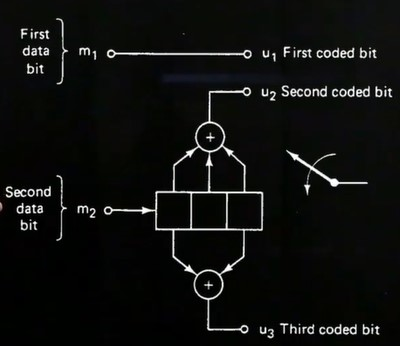
\includegraphics[width=1\textwidth]{images/trellis/trellis_example1.jpg}
        \caption{convolutional code}\label{subfig:convolutional_code}
    \end{subfigure}
    \hfil
    \begin{subfigure}[t]{0.49\linewidth}
        \centering
        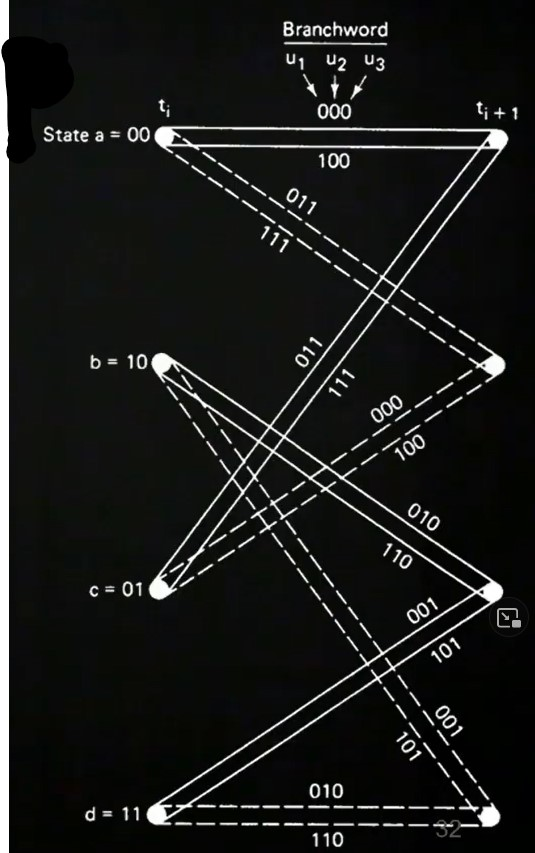
\includegraphics[width=0.6\textwidth]{images/trellis/trellis_example2.jpg}
        \caption{trellis1}\label{subfig:trellis1}
    \end{subfigure}
    \begin{subfigure}[t]{0.49\linewidth}
        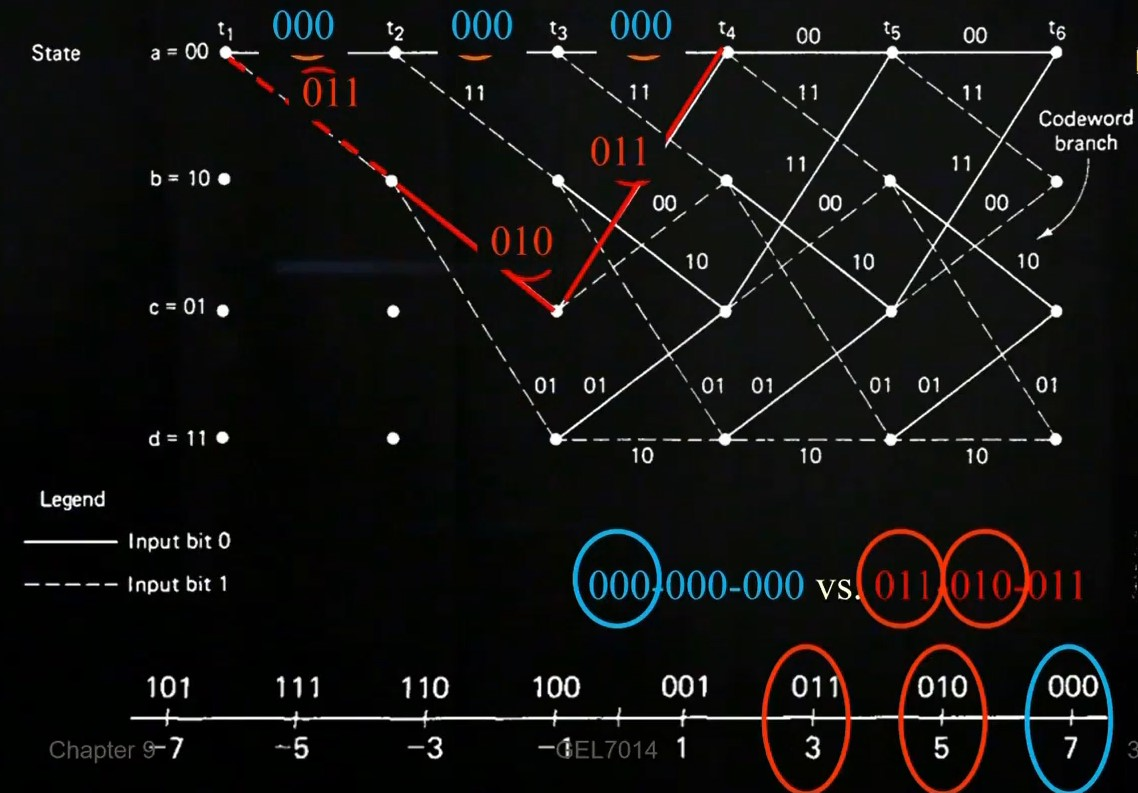
\includegraphics[width=1\textwidth]{images/trellis/trellis_example3.jpg}
        \caption{trellis2}\label{subfig:trellis2}
    \end{subfigure}
    \hfil
    \begin{subfigure}[t]{0.4\linewidth}
        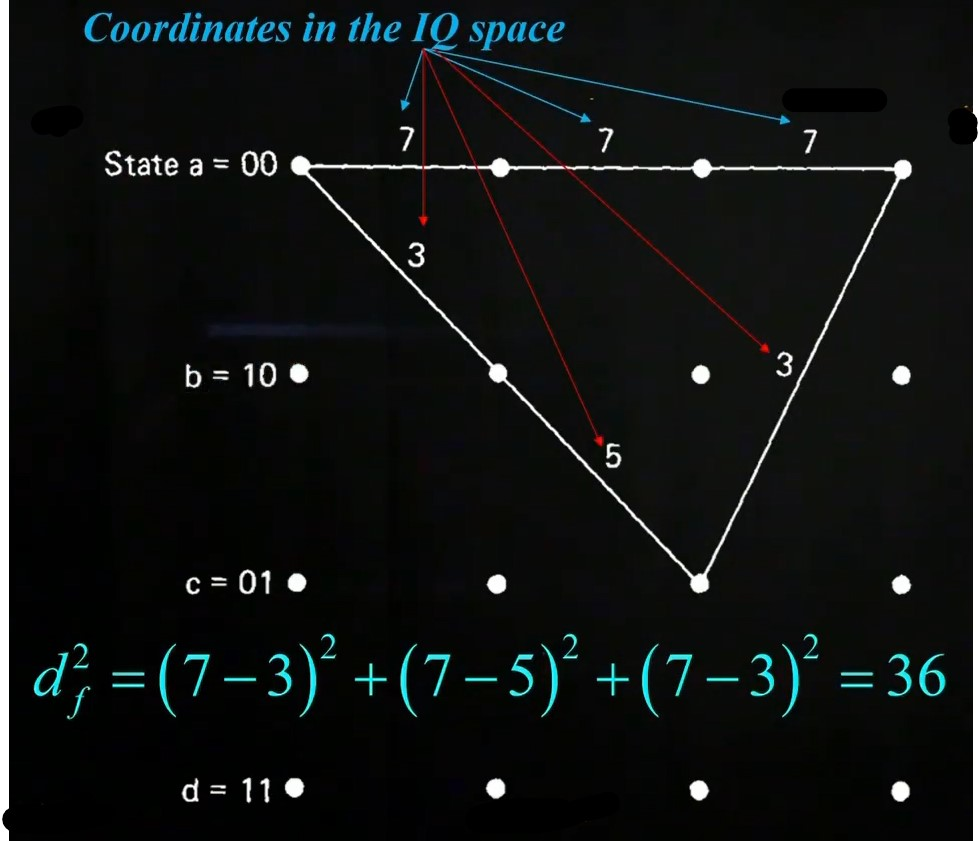
\includegraphics[width=1\textwidth]{images/trellis/trellis_example4.jpg}
        \caption{$d_{\text {free,coded }}^2$}\label{subfig:free_coded}
    \end{subfigure}
    \centering
    \begin{subfigure}[t]{0.49\linewidth}
        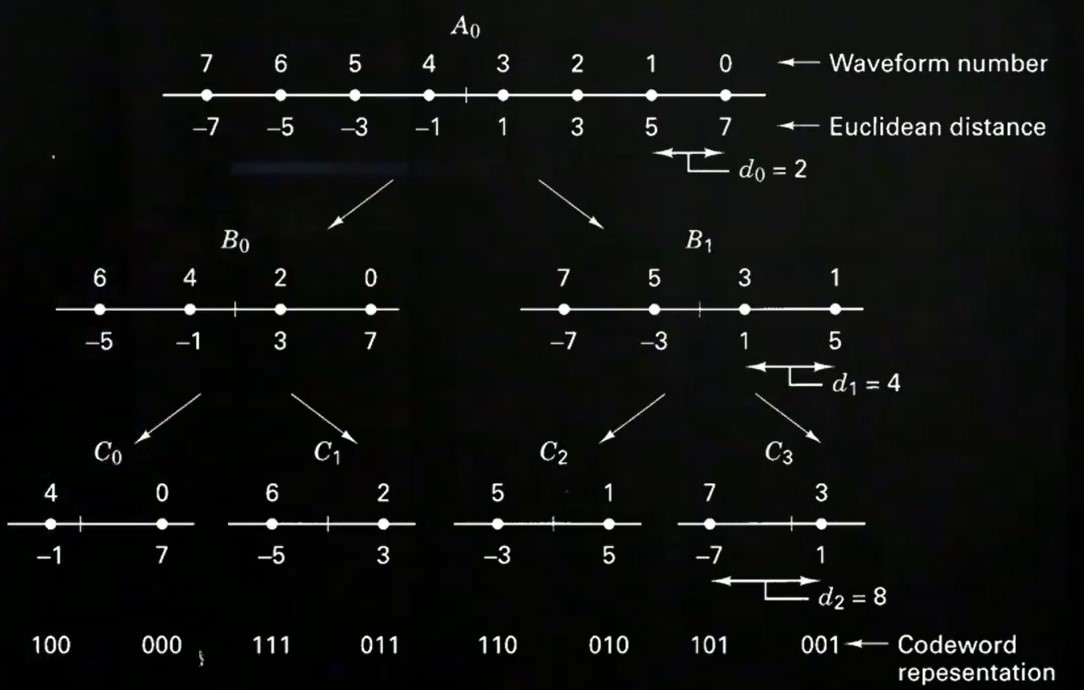
\includegraphics[width=1\textwidth]{images/trellis/trellis_example5.jpg}
        \caption{set-partitoning}\label{subfig:set_partitioning}
    \end{subfigure}
\caption{trellis}
\label{fig:ex_trellis}
\end{figure}
\FloatBarrier 
\subsubsection{1/2 QPSK TCM}
1/2 mans one has one input and two outputs.
\begin{equation}
    \begin{array}{rrrrrr}
    \hline \tilde{m} & \text { number of states } & m & \text { rate } & \text { constellation } & \text { asympt. gain } G \\
    \hline 1 & 2 & 1 & 1 / 2 & \text { BPSK/QPSK } & 1.76 \mathrm{~dB} \\
    1 & 2 & 2 & 2 / 3 & \text { QPSK/8-PSK } & 1.1 \mathrm{~dB}  \\
    1 & 4 & 2 & 2 / 3 & \text { QPSK/8-PSK } & 3.0 \mathrm{~dB}   \\
    2 & 8 & 2 & 2 / 3 & \text { QPSK/8-PSK } & 3.6 \mathrm{~dB}   \\
    2 & 8 & 3 & 3 / 4 & 8 \text {-PSK/16-PSK } & 3.98 \mathrm{~dB}  \\
    \hline
    \end{array}
\end{equation}
\subsubsection{Function}
The number of states of a trellis is always given by two to the power of number of storage elements, for example \autoref{fig:pdf2} has two states, since $2^1=2$. The coding gain G is given by \autoref{eq:coding_gain}.
\begin{equation}\label{eq:coding_gain}
G=\frac{d_{\text {free,coded }}^2}{d_{\text {min,uncoded }}^2}
\end{equation}
When one wants to calculate the coding gain for a two-state 2/3 TCM with QPSK one gets the following result:
$$
G=\frac{2.5858}{2}=1.2929=1.12 \mathrm{~dB}
$$
This is because the shortest distance squared in QPSK is 2, see also \autoref{fig:shortest_path1}, when one sends one bit the shortest distance squared is two, since one would go from position zero to position two in \autoref{fig:shortest_path1}. In a two-state 2/3 TCM it looks different, one has a storage element, due to that the signal looks like in \autoref{fig:shortest_path2} when one changes the LSB. This results in a total distance of $d_{\text {free }}^2=d^2(0,2)+d^2(0,1)=2+(2-\sqrt{2})=2.5858$ (Note to calculate the distance one always refers to zero as it is also done in \autoref{sbusubsec:example_pam}). When one would change the most significant bit the distance would be even higher, since one jumps always to the other side of the circle. 
\begin{figure}[ht]
    \begin{subfigure}[t]{0.3\linewidth}
        \resizebox{1\textwidth}{!}{\subimport{images/}{trellis1.tex}}
        \caption{state 0}\label{subfig:qpsk}
    \end{subfigure}
 \hfil
    \begin{subfigure}[t]{0.3\linewidth}
        \resizebox{1\textwidth}{!}{\subimport{images/}{trellis2.tex}}
        \caption{state 1}\label{subfig:8-psk}
    \end{subfigure}
    
\caption{QPSK shortest path}
\label{fig:shortest_path1}
\end{figure}
\begin{figure}[ht]
    \begin{subfigure}[t]{0.3\linewidth}
        \resizebox{1\textwidth}{!}{\subimport{images/}{trellis1.tex}}
        \caption{state 0}\label{subfig:qpsk}
    \end{subfigure}
    \hfil
    \begin{subfigure}[t]{0.3\linewidth}
        \resizebox{1\textwidth}{!}{\subimport{images/}{trellis2.tex}}
        \caption{state 1}\label{subfig:8-psk}
    \end{subfigure}
    \hfil
    \begin{subfigure}[t]{0.3\linewidth}
        \resizebox{1\textwidth}{!}{\subimport{images/}{trellis3.tex}}
        \caption{state 2}\label{subfig:8-psk}
    \end{subfigure}
    
\caption{two-state 2/3 TCM shortest path}
\label{fig:shortest_path2}
\end{figure}

\begin{figure}[ht]
    \centering
        %trim=left botm right top
        \includegraphics[page=135, clip, trim=6cm 17cm 4.5cm 7.5cm, width=0.8\textwidth]{data/99_TSM_SignProc LectureNotes 2022 part1.pdf}
    \caption{Minimum (squared) Euclidean distance in a constellation plot (unit circle) for 8-PSK.}
    \label{fig:pdf1}
\end{figure}
\begin{figure}[ht]
    \centering
        %trim=left botm right top
        \includegraphics[page=137, clip, trim=6cm 19cm 4.5cm 8.2cm, width=0.8\textwidth]{data/99_TSM_SignProc LectureNotes 2022 part1.pdf}
    \caption{Encoder for the constellation index for a two-state rate 2/3 TCM.}
    \label{fig:pdf2}
\end{figure}
\begin{figure}[ht]
    \centering
        %trim=left botm right top
        \includegraphics[page=137, clip, trim=5.5cm 10.5cm 4.5cm 15cm, width=0.8\textwidth]{data/99_TSM_SignProc LectureNotes 2022 part1.pdf}
    \caption{Trellis for a two-state rate $2 / 3$ TCM including parallel transitions, $\boldsymbol{y}=y_2 y_1 y_0$.}
    \label{fig:pdf3}
\end{figure}
\begin{figure}[ht]
    \centering
        %trim=left botm right top
        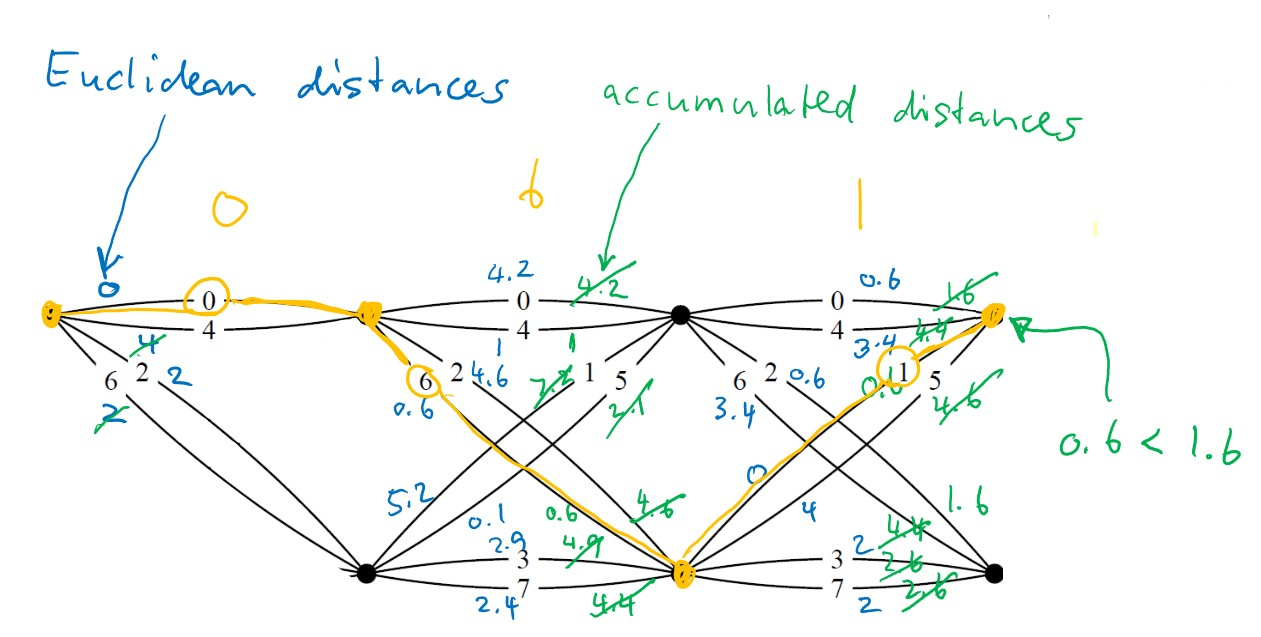
\includegraphics[width=0.8\textwidth]{images/trellis_example.jpg}
    \caption{Example}
    \label{fig:example_trellis}
\end{figure}

\subsubsection{Example two state 2/3 Trellis modulation}
See also the following \href{https://youtu.be/rnjy4_gXLAg}{video}. We have an input signal $x_1=\{0,1,0\}$ and $x_2=\{0,1,0\}$ and the received values are $n_1=0, n_2=-0.8+j, n_3=0$. We start at state zero and calculate now the distances to the other states. Since we received zero in the beginning, the squared distance  to zero is zero, to four four, to two two and to six also two. In the next state we received $-0.8+j$, therefore, the distance to zero is $(1--0.8)^2+(0-1)^2=4.24$, to point four $(-1--0.8)^2+(0-1)^2=1.04$, to point one $(\sqrt{2}--0.8)^2+(\sqrt{2}-1)^2=5.07$ and so on. for the last received signal one can do again the same. In the end one decides for the path which has the least squared distance, which is 0,6,1. This is also what was sent according to \autoref{tb:trellis}. The whole diagram can be found in \autoref{fig:example_trellis}
\begin{table}[h!]
\centering
 \begin{tabular}{||c c c c||} 
 \hline
 Bit & State1 & State2 & State3 \\ [0.5ex] 
 \hline\hline
 MSB & 0 & 1 & 0 \\ 
  & 0 & 1 & 0 \\
 LSB & 0 & 0 & 1 \\
 Result & 0 & 6 & 1 \\
 \hline
 \end{tabular}
 \label{tb:trellis}
 \end{table}
% \begin{figure}[ht]
%     \centering
%         %trim=left botm right top
%         \includegraphics[page=138, clip, trim=5cm 16.9cm 4.5cm 10cm, width=0.8\textwidth]{data/99_TSM_SignProc LectureNotes 2022 part1.pdf}
%     \caption{Encoder for a four-state rate 2/3 TCM.}
%     \label{fig:pdf4}
% \end{figure}
% \begin{figure}[ht]
%     \centering
%         %trim=left botm right top
%         \includegraphics[page=138, clip, trim=5.5cm 7cm 4.5cm 14cm, width=0.8\textwidth]{data/99_TSM_SignProc LectureNotes 2022 part1.pdf}
%     \caption{State diagram for a four-state TCM.}
%     \label{fig:pdf5}
% \end{figure}
% \begin{figure}[ht!]
%   \centering
%   \resizebox{0.8\textwidth}{!}{\subimport{images/}{trellis.tex}}
%   \caption{Trellis}
%   \label{fig:trellis}
% \end{figure}
\FloatBarrier 
\section{Modulation Variants}
entropy:
\begin{equation}
H(Y) \triangleq-\int_{-\infty}^{\infty} p(y) \log _2 p(y) d y
\end{equation}
conditional entrpy:
\begin{equation}
H(Y \mid X) \triangleq-\int_{-\infty}^{\infty} p(x) \int_{-\infty}^{\infty} p(y \mid x) \log _2 p(y \mid x) d y d x
\end{equation}
The capacity is then given as:
\begin{equation}
C=I(X ; Y)=H(Y)-H(Y \mid X)
\end{equation}
When one has a gaussian distributed signal and gausian distributet noise the max capacity is given with the formula below.
\begin{equation}
C=\frac{1}{2} \log _2\left(1+\frac{E_s}{\sigma^2}\right)
\end{equation}
For a discrete memoryless channel (DMC) the following applies.
\begin{equation}
C_{\mathrm{DMC}}=\max _{p(k)} \sum_{k=1}^K \sum_{j=1}^J p(j \mid k) p(k) \log _2 \frac{p(j \mid k)}{p(j)}
\end{equation}
where p(x) is the distribution for example zero and one with a dirac of 1/2 at each point.
Numerical evalution for the capacity.
\begin{equation}
=\frac{E_s}{\sigma^2} \log _2 \mathrm{e}-\frac{1}{\sqrt{2 \pi} \sigma} \mathrm{e}^{-\frac{E_s}{2 \sigma^2}} \int_{-\infty}^{\infty} \mathrm{e}^{-\frac{y^2}{2 \sigma^2}}\left(\cosh \frac{y \sqrt{E_s}}{\sigma^2}\right) \log _2\left(\cosh \frac{y \sqrt{E_s}}{\sigma^2}\right) d y .
\end{equation}

\begin{figure}[ht]

    \begin{subfigure}[t]{0.3\linewidth}
  \resizebox{1\textwidth}{!}{\subimport{images/}{QPSK.tex}}
\caption{QPSK}\label{subfig:qpsk}
    \end{subfigure}
 \hfil
    \begin{subfigure}[t]{0.3\linewidth}
\resizebox{1\textwidth}{!}{\subimport{images/}{8-PSK.tex}}
\caption{8-PSK}\label{subfig:8-psk}
    \end{subfigure}
\hfil
    \begin{subfigure}[t]{0.3\linewidth}
 \resizebox{1\textwidth}{!}{\subimport{images/}{16-PSK.tex}}
\caption{16-PSK}\label{subfig:16-psk}
    \end{subfigure}

    \begin{subfigure}[t]{0.3\linewidth}
\resizebox{1\textwidth}{!}{\subimport{images/}{16-QAM.tex}}
\caption{16-QAM}\label{subfig:16-qam}
    \end{subfigure}
    \hfil
    \begin{subfigure}[t]{0.69\linewidth}
\resizebox{1\textwidth}{!}{\subimport{images/}{m-pam.tex}}
\caption{8-PAM}\label{subfig:16-qam}
    \end{subfigure}
%
\caption{Constellation diagrams}
\end{figure}
\FloatBarrier 
\subsection{Symbol Energy, Bit Energy}
The average symbol and Bit energy in QAM and PSK is given by \autoref{eq:qam_psk_engergy}.
\begin{equation} \label{eq:qam_psk_engergy}
\begin{aligned}
& E_s=\frac{1}{M} \sum_{m=0}^{M-1}\left|\underline{s}_m\right|^2 \quad \frac{\text { Joules }}{\text { Symbol }} \\
& E_b=\frac{1}{\log_2(M)} E_s \quad \frac{\text { Joules }}{\text { bit }}
\end{aligned}
\end{equation}
Where:
\begin{itemize}
    \item M, is the number of points in the signal constellation. (for example in \autoref{fig:rectangular_quam} M=8)
    \item $\underline{s}_m$ one specific Symbol out of M
    \item $E_s$ ,is the average symbol energy
    \item $E_b$, is the average bit energy (it is divided by $\log_2(M)$ because with $2^M$ symbols one can transmit $M$ bits)
\end{itemize}
\FloatBarrier 
\subsubsection{Example Calculate bit and signal energy of M=8 rectangular QAM}
Given is the M=8 rectangular QAM that can be seen in \autoref{fig:rectangular_quam}
\begin{figure}[ht!]
  \centering
  \resizebox{8cm}{!}{\subimport{images/}{rectangular_quam.tex}}
  \caption{M=8 rectangular QAM for example}
  \label{fig:rectangular_quam}
\end{figure}
now one wants to calculate $E_s,E_b$. This can be done with \autoref{eq:qam_psk_engergy} this gives the following result (see also the following \href{https://youtu.be/Z3wHXSCrlSM}{video}).
$$
\begin{aligned}
E_s &=\frac{1}{M} \sum_{m=0}^{M-1}\left|\underline{s}_m\right|^2 \quad \frac{\text { Joules }}{\text { Symbol }}\\
& =\frac{1}{8}\left[\left(A^2+A^2\right) 4+\left((3 A)^2+A^2\right) 4\right] \\
& =\frac{1}{8}\left[8 A^2+40 A^2\right] \\
& =\frac{48}{8} A^2=6 A^2 \\
E_b & =\frac{6 A^2}{\log _2 8}=2 A^2
\end{aligned}
$$
Where:
\begin{itemize}
    \item A=Amplitude
\end{itemize}
\FloatBarrier 
\subsubsection{Example M-PAM/M-PSK based TCM}
\paragraph{Example derive the minimum Euclidean distance $d^2_{min}$ in an M-array PAM system, whose power has been normalized to one}\mbox{}\newline
\label{par:m-pam_power}
With \autoref{eq:qam_psk_engergy} one can calculate the energy per symbol (as a reference also have a look at \autoref{fig:m-pam}):
\begin{figure}[ht!]
  \centering
  \resizebox{10cm}{!}{\subimport{images/}{m-pam.tex}}
  \caption{M=8 PAM example}
  \label{fig:m-pam}
\end{figure}
$$
\begin{aligned}
E_s&=\frac{1}{M} \sum_{m=0}^{M-1}\left|\underline{s}_m\right|^2 \quad \frac{\text { Joules }}{\text { Symbol }}\\
& =\frac{1}{M} \cdot 2 \sum_{m=1}^{M / 2}((2 m-1) A)^2 \\
& =\frac{2 A^2}{M} \sum_{m=1}^{M / 2}(2 m-1)^2 \\
& =\frac{2 A^2}{M}\left(4 \sum_{m=1}^{M / 2} m^2-4 \sum_{m=1}^{M / 2} m+\sum_{m=1}^{M / 2} 1\right) \\
& =\frac{2 A^2}{M}\left(\frac{M(M+2)(M+1)}{6}-\frac{M(M+2)}{2}+\frac{M}{2}\right) \\
& =\frac{A^2}{3}\left(M^2-1\right)
\end{aligned}
$$
Since we want P = 1, we get
$$
A=\sqrt{\frac{3}{M^2-1}}
$$
Therefore 
$$
d_{\min }^2=(2\cdot A)^2=\frac{12}{M^2-1}
$$
\paragraph{Derive the general expression for the minimum Euclidean distance $d^2_{min}$ in an M-array PSK system}\mbox{}\newline
With \autoref{eq:qam_psk_engergy} one can calculate the energy per symbol
$$
\begin{aligned}
E_s&=\frac{1}{M} \sum_{m=0}^{M-1}\left|\underline{s}_m\right|^2 \quad \frac{\text { Joules }}{\text { Symbol }}\\
& =\frac{1}{M} \sum_{m=0}^{M}(A)^2\\
&=A^2
\end{aligned}
$$
Since we want P = 1, we get
$$
A=1
$$
\begin{figure}[ht]
\centering
    \begin{subfigure}[t]{0.3\linewidth}
        \resizebox{1\textwidth}{!}{\subimport{images/}{octagon.tex}}
        \caption{Octagon}\label{subfig:octagon}
    \end{subfigure}
 \hfil
 \centering
    \begin{subfigure}[t]{0.3\linewidth}
        \resizebox{1\textwidth}{!}{\subimport{images/}{triangle2.tex}}
        \caption{Triangle for cosine rule}\label{subfig:triangle2}
    \end{subfigure}
\caption{Help for cosine rule}
\label{fig:help_cosine_rule}
\end{figure}
% \begin{figure}[ht!]
%   \centering
%   \resizebox{6cm}{!}{\subimport{images/}{octagon.tex}}
%   \caption{Octagon}
%   \label{fig:octagon}
% \end{figure}
% \begin{figure}[ht!]
%   \centering
%   \resizebox{10cm}{!}{\subimport{images/}{triangle2.tex}}
%   \caption{Triangle for cosine rule}
%   \label{fig:triangle2}
% \end{figure}
\begin{equation}\label{eq:cosine_rule}
\cos (A)=\frac{b^2+c^2-a^2}{2 b c}
\end{equation}
With this and the cosine (\autoref{eq:cosine_rule}) rule one gets the following result (to get the idea with the cosine rule also have a look at \autoref{fig:help_cosine_rule}).
$$
\cos \left(\frac{2\cdot \pi}{M} \right)=\frac{2\cdot A^2-d^2_{min}}{2 \cdot A^2} \Rightarrow \cos \left(\frac{2\cdot \pi}{M} \right) \cdot 2 \cdot A^2 - 2 \cdot A^2=-d^2_{min} \Rightarrow d^2_{min}= 2 \cdot A^2 \left(1-\cos \left(\frac{2\cdot \pi}{M} \right)\right)=2 \left(1-\cos \left(\frac{2\cdot \pi}{M} \right)\right)
$$
\section{Smart Antenna Systems}
Smart is not the antenna itself, but the signal processing behind it. Smart antennas can be divided in switched beam antennas and adaptive array antenna. Typical applications are DOA(Direction of arrival) and beamforming.
\subsection{Phased array}
One has multiple antennas with different phases, therefore negative and positive interference happens, which leads to the fact that one only has radiation in a certain direction. SDMA (Space division multiple access). Adaptive beam former for SDMA are useful because one can suppress interferer, whereas with a switched arrays this is not possible, since the negative interference always happens at the same place/angle.
\subsection{The phased array principle}
In this principle we assume that the signals are emitted from several psitions $\overrightarrow{x_n}$ with the wave propagation constant $k=\frac{2\pi}{\lambda}$

The phase shift at the location $\overrightarrow{y}$ can be calculated according to \autoref{eq:general_superimposed_signal}.
\begin{equation}\label{eq:general_superimposed_signal}
\Delta \varphi=-k\left|\overrightarrow{x_n}-\vec{y}\right|
\end{equation}
The superimposed (complex) signal $\underline{g}$ at point $\overrightarrow{y}$ can be calculated according to the following formulas:
\begin{equation}\label{eq:superimposed_complex_signal}
\underline{g}(\vec{y})=\sum_{n=0}^{N-1} \underline{w}_n \cdot g_n(\phi) \cdot \exp \left(-\mathrm{j} \cdot \mathrm{k}\left|\overrightarrow{x_n}-\vec{y}\right|\right)
\end{equation}
\begin{itemize}
    \item $g_n(\phi)$ directivit of the $n_{th}$ source
    \item $\overrightarrow{x_n}$ location of the $n_{th}$ source (transmitter)
    \item $y$ location of the receiver
    \item $\underline{w}_n$ complex amplitude of the $n_{th}$ source feed
\end{itemize}
Note that the exponential term is only the rotation of the signal.
\subsubsection{Uniform linear array}
From \autoref{eq:general_superimposed_signal} one has seen that the callculation for an array antenna can become quite difficult. But when the antennas are distributed in an equal distance d one gets \autoref{eq:superimposed_signal_equal_distribution}.
\begin{equation}\label{eq:superimposed_signal_equal_distribution}
\underline{g}(\phi)=\sum_{n=0}^{N-1} \underline{w}_n \cdot g_n(\phi) \cdot \exp (-\mathrm{j} \cdot \mathrm{k} \cdot n \cdot d \cdot \sin \phi)
\end{equation}
Which is just the discrete Fourier transform. n describes again the n'th antenna element and $\phi$ the angle (when one stands before the antenna $\phi$ is zero, when one stands next to the antenna array (left or right) the angle is 90 degree).
\subsection{Broadside Array}
In a broadside array, all currents are the same. According to geometric progression one can also write:
\begin{equation}
\begin{aligned}
&\underline{g_g}(\phi)=\underline{w}_0 \cdot \frac{1-e^{-j N k d \sin \phi}}{1-e^{-j k d \sin \phi}} \\
&\left|\underline{g_g}(\phi)\right|=\left|\underline{w}_0\right| \cdot \frac{\left|\sin \left[\frac{1}{2}(N k d \sin \phi)\right]\right|}{\left|\sin \left[\frac{1}{2}(k d \sin \phi)\right]\right|}
\end{aligned}
\end{equation}
And below the trigonometric ratios
\begin{equation}
\begin{aligned}
\sin (\theta) &=\frac{o p p}{h y p} \\
\cos (\theta) &=\frac{a d j}{h y p} \\
\tan (\theta) &=\frac{o p p}{a d j}
\end{aligned}
\end{equation}
\begin{figure}[ht]
  \centering
  \resizebox{0.5\textwidth}{!}{\subimport{images/}{trigonometrie.tex}}
  \caption{Trigonometry}
  \label{fig:trig}
\end{figure}
Peaks occur when \autoref{eq:peaks} is fulfilled. $\Rightarrow \phi=0$. Furthermore the Bandwidth can be callculated according to \autoref{eq:Bandwidth}.
\begin{equation}\label{eq:peaks}
k \cdot d \cdot \sin \phi_p=0
\end{equation}
\begin{equation}\label{eq:Bandwidth}
B=2 \cdot \phi_z=2 \sin ^{-1}\left(\frac{\lambda}{N \cdot d}\right) \approx \frac{2 \cdot \lambda}{L}
\end{equation}
\paragraph{Group Pattern}\mbox{}\\
Draft the group pattern of 2 radiators having a distance of d=0.75$\lambda$. Determine the nulls.\newline

Furthermore, note that the distance between two radiators must exceed 0.5 $\lambda$ otherwise problems occur.
\begin{figure}[ht]
  \centering
  \resizebox{0.5\textwidth}{!}{\subimport{images/}{triangle.tex}}
  \caption{Triangle}
  \label{fig:triang}
\end{figure}
With \autoref{fig:triang} one can calculate the angle x which is $cos^{-1}(\frac{0.5}{0.75})=0.841=\underline{\underline{48.19^{\circ}}}$, the same would be true when one goes in the other direction $180^{\circ}-48.19^{\circ}=\underline{\underline{131.81^{\circ}}}$. Note: 0.5 was chosen since then one has negative interference.


\paragraph{Directivity in patch antenna arrays}\mbox{}\\
Explain why it is difficult to obtain a high directivity for large $\Phi$ (see presentation) for patch
arrays. Suggest an alternative construction.\newline

It is difficult, since the sine of $\frac{\pi}{2}$ is always zero. an alternative solution would be to rotate the whole antenna by 90 degree. Or to place them on a non-planar carrier.
\paragraph{Directivity and grating lobes}\mbox{}\\
Explain why the directivity usually decreases when grating lobes occur.

Grating lobes mean that a substantial part of the energy is radiated in these directions. This energy of course is not available any more to be radiated in the main direction which defines the directivity of the antenna. Therefore, the directivity decreases
\paragraph{Beamwitdh}
Estimate the beamwidth (in degrees) of a 10 element broadside array at 5GHz if the antenna elements are considered as isotropic radiators fed with equal signals and the distances between the neighboured elements are 0.5$\lambda$ \newline
According to \autoref{eq:Bandwidth} the beamwidth can be calculated as follows:

$$
2 \phi_z \approx 2 \cdot \sin ^{-1}\left(\frac{\lambda}{N d}\right) \approx \frac{2 \lambda}{L}
$$
Therefore
$$
\begin{aligned}
&\lambda / \mathrm{d}=2 \\
&\mathrm{~N}=10 \\
&\Rightarrow 2 \Phi_{\mathrm{z}}=2 \sin ^{-1}(1 / 5) \approx 23^{\circ}
\end{aligned}
$$
\subsubsection{Exercise Smart Antenna}
\textbf{Consider two isotropic radiators located at a distance of d=0.55$\lambda$. Both radiators are driven by a sinusoidal carrier signal with equal amplitude. The phase of the signal feeding radiator 1 lags behind  the signal of radiator 2 by 60$^{\circ}$. Calculate the angle $\alpha$, at which there is a zero of the radiation.}
$$
\cos(\beta)\cdot d + \frac{1}{6}=0.5 \Rightarrow \beta = 52.7^{\circ} \Rightarrow \alpha=180^{\circ}-52.7^{\circ}=127.3^{\circ}
$$
\begin{figure}[ht!]
  \centering
  \resizebox{12cm}{!}{\subimport{images/}{smart_antenna}}
  \caption{Resulting wave}
  \label{fig:smart_antenna}
\end{figure}

\section{Transceiver}
In the past the number of components was important for transceivers, whereas today it's chip area. Since it is not possible to build a very shallow bandpass filter with only a few components, different transceivers were developed in the past. 
\subsection{Heterodyne Receiver and Image Rejection}
One of them was the superheterodyne receiver, which multiplies the receiving signal with a local oscillator signal as it can be seen in \autoref{fig:typical_superheterodyne_receiver}. Thereby, the lower resulting frequency is often called intermediate frequency ($\omega_{IF}$ or $f_{IF}$).

The bandpass at the beginning of \autoref{fig:typical_superheterodyne_receiver} is used to suppress out-of-band signals. Furthermore, an amplifier is present which might cause issues when the signal is to strong since the amplifier is then not working in its linear region any more. The amplifier is needed because of the mixer, since the mixer has an insertion loss. The IF bandpass filter is used filter out unwanted frequencies and to select the correct channel. To change the receiving frequency one has to changes the oscillator frequency, since the second bandpass is normally constant.\newline
So the RF bandpass is used to do the band selection and remove the image frequency and the if bandpass selects the channel. Sometimes there are two RF filters (one before and one after the amplifier) this is done to keep the insertion loss quite low. $\Rightarrow$ first filter is not very good, but has nearly no insertion loss second filter has more insertion loss, but signal was already amplified.\newline
The different symbols mean the following:
\begin{itemize}
    \item $\omega_{IF}$ = intermediate frequency (difference between $\omega_{LO}$ and $\omega_{RF}$)
    \item $\omega_{LO}$ = local oscillator
    \item $\omega_{RF}$ = radio frequency signal
\end{itemize}
\begin{figure}[ht]
  \centering
  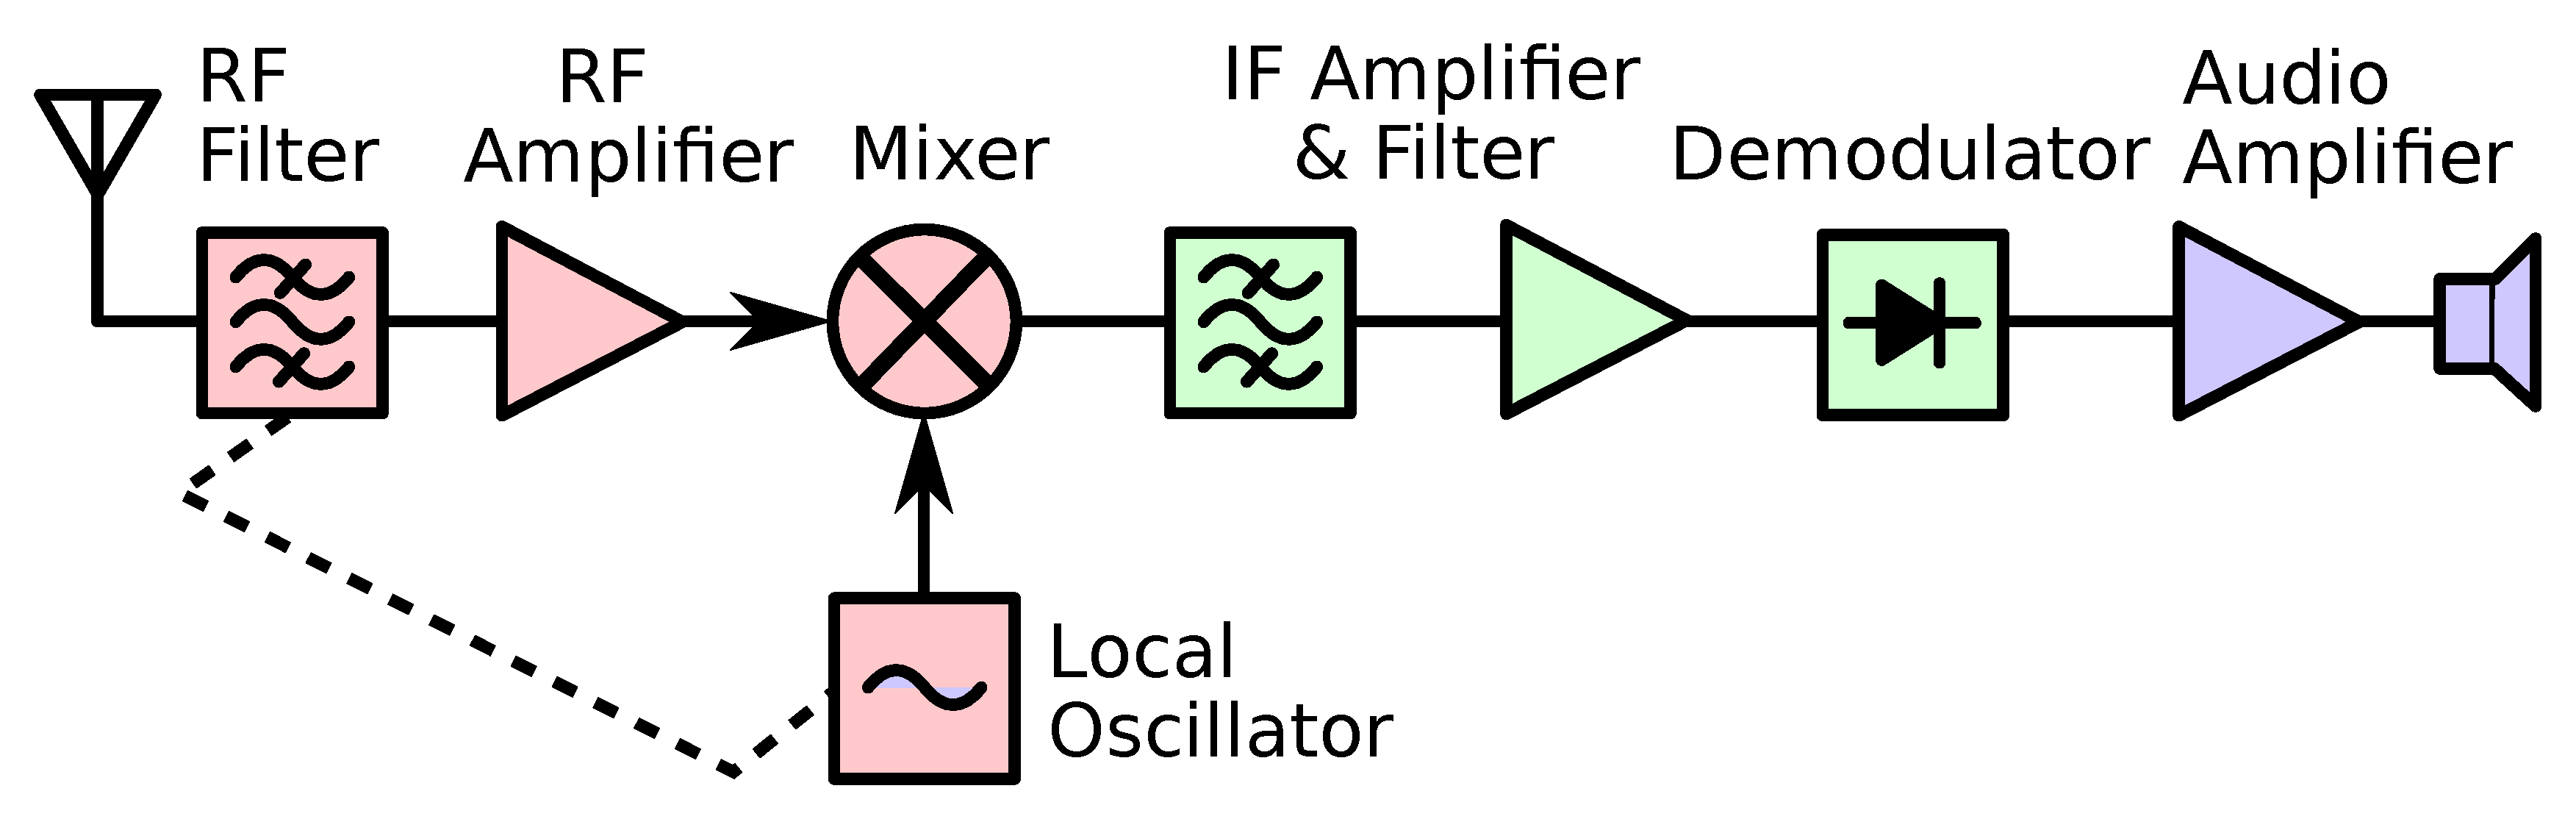
\includegraphics[width=8cm]{images/Superheterodyne1.pdf}
  \caption{typical superheterodyne receiver}
  \label{fig:typical_superheterodyne_receiver}
\end{figure}
\subsubsection{Mixing Processes}\mbox{}\\
To design a superheterodyne receiver, one must be familiar with the trigonometric identities especially with the product identities, which can be seen in \autoref{eq:trigonometric_product_identity}. From those one can then derive \autoref{eq:mixer_output}.
\begin{equation}\label{eq:trigonometric_product_identity}
\begin{aligned}
\sin \alpha \cos \beta &=\frac{\sin (\alpha+\beta)+\sin (\alpha-\beta)}{2} \\
\cos \alpha \cos \beta &=\frac{\cos (\alpha+\beta)+\cos (\alpha-\beta)}{2} \\
\sin \alpha \sin \beta &=\frac{\cos (\alpha-\beta)-\cos (\alpha+\beta)}{2}
\end{aligned}
\end{equation}
\begin{equation}\label{eq:mixer_output}
f_{I F}=\left|f_{R F} \pm f_{L O}\right|
\end{equation}
Due to the properties derived in the formulas above, one could think it's super easy to to get a RF signal to a lower one. The only issue one has is that the received signal is not ideal, one has always some noise on it and one can not create ideal bandpass filters. Which means when $\omega_{LO}$ is chosen to small and the bandpass is to large the new signal on the frequency $\omega_{LO}$ is overlapped by the image frequency (frequency which is mapped to the same $f_{IF}$ as the $f_{RF}$ signal). \newline For example in \autoref{fig:image_freq_1} when we choose $f_{LO}$ to be $f_{LO_1}$ the $f_{RF}$ and $f_{IM_1}$ produce the frequency $f_{IF}$ according to \autoref{eq:mixer_output}. Due to that, one needs a bandpass filter as it can be seen in \autoref{fig:image_freq_2}. There the bandpass filter is not ideal and still some noise from $f_{IM_1}$ superimposes the signal on $f_{IF}$. In \autoref{fig:image_freq_1} and \autoref{fig:image_freq_2} one also sees the smaller $\omega_{IF}$ gets the better the bandpass must be. Furthermore one sees that the image frequency is given by \autoref{eq:image_frequency}.
\begin{equation}\label{eq:image_frequency}
f_{I M}=f_{R F} \pm 2 f_{I F}
\end{equation}
\begin{figure}[ht]
  \centering
  \resizebox{1\textwidth}{!}{\subimport{images/}{spectrum_3.tex}}
  \caption{Image frequencies without bandpass}
  \label{fig:image_freq_1}
\end{figure}
\begin{figure}[ht]
  \centering
  \resizebox{1\textwidth}{!}{\subimport{images/}{spectrum_4.tex}}
  \caption{Image frequencies with bandpass}
  \label{fig:image_freq_2}
\end{figure}


\subsubsection{Zero-if conversion}
A direct-conversion receiver (DCR), also known as homodyne, synchrodyne, or zero-IF receiver, is a radio receiver design that demodulates the incoming radio signal using synchronous detection driven by a local oscillator whose frequency is identical to, or very close to the carrier frequency of the intended signal. The benefit is that one does not have image frequencies and no need of huge analogue filters is needed. The drawback is the receiver topology is more complicated. One needs to do a hilbert transform. Exactly 90 degree phase shift is required.\newline Direct multiplying the RF input signal is only possible when \autoref{eq:direct_conversion} is fullfilled.
\begin{equation}\label{eq:direct_conversion}
\underline{S}\left(f_c-\Delta f\right)=\underline{S}^*\left(f_c+\Delta f\right)
\end{equation}

For example one has the signal $(\sin (x \times 2)+\sin (x \times 2.1)-\sin (x \times 1.9))$ and want to transform it with this mehtod, therefore one multiplies it with $\sin (2 x)$ which results in the following:  $\sin (2 x)(\sin (x \times 2)+\sin (x \times 2.1)-\sin (x \times 1.9))$ which results in the following: $\frac{1}{2}(-\cos (4.1 x)-\cos (4 x)+\cos (3.9 x)+1)$ from which one can see  that some part of the signal is missing in the baseband. But when also doing the multiplication with a 90 degree pahse shifted signal one also gets this part as it can be seen in the following: $\cos (2 x)(\sin (x \times 2)+\sin (x \times 2.1)-\sin (x \times 1.9))$ which is $\frac{1}{2}(\sin (4.1 x)+\sin (4 x)-\sin (3.9 x)+2 \sin (0.1 x))$
$$
\begin{aligned}
    &\cos (2\cdot \omega)(\sin (2\cdot \omega)+\sin (2.1\cdot \omega)-\sin (1.9\cdot \omega))&=\frac{1}{2}(\sin (4.1\cdot \omega)+\sin (4\cdot \omega)-\sin (3.9\cdot \omega)+2 \sin (0.1\cdot \omega))\\
    &\cos (2\cdot \omega)(\sin (2\cdot \omega)-\sin (2.1\cdot \omega)+\sin (1.9\cdot \omega))&=\frac{1}{2}(\sin (4.1\cdot \omega)+\sin (4\cdot \omega)-\sin (3.9\cdot \omega)-2 \sin (0.1\cdot \omega))\\
\end{aligned}
$$
$$
\begin{aligned}
    &e^{-2 i \omega}(\sin (1.9 \omega)+\sin (2 \omega)-\sin (2.1 \omega)) =\frac{1}{2} i e^{-4 i \omega}-\frac{1}{2} i e^{(-0.1 i) \omega}+\frac{1}{2} i e^{(0.1 i) \omega}+\frac{1}{2} i e^{(-3.9 i) \omega}-\frac{1}{2} i e^{(-4.1 i) \omega}+-\frac{i}{2}\\
    &=\frac{1}{2} i(2 i \sin (0.1 \omega)-i \sin (3.9 \omega)-i \sin (4 \omega)+ i \sin (4.1 \omega)+\cos (3.9 \omega)+\cos (4 \omega)-\cos (4.1 \omega)-1)\\
\end{aligned}
$$

\paragraph{Broadband phase shifting}
\begin{enumerate}
    \item Show that a broadband 90$^{\circ}$ phase shifting can be realized using the circuit topology in \autoref{fig:phase_shifter}
    $$
    \underline{T_1}=\frac{U_2}{\underline{U}_1}=\frac{1}{1+j \omega R C}
    $$
    $$
    \underline{T_2}=\frac{\underline{U}_2^{\prime}}{\underline{U_1^{\prime}}}=\frac{j \omega R C}{1+j \omega R C}
    $$
    $$
    \varphi=\arg \left\{\underline{I}_2\right\}-\arg \left\{\underline{T}_1\right\}=90^{\circ}-\arctan \{\omega R C\}-(-\arctan \{\omega R C\})=90^{\circ}, \forall \omega
    $$
    \item What would be the amplitude characteristics without limiting amplifiers?
    $$
    \left|\frac{T_2}{T_1}\right|=\omega R C
    $$
    $$
    \Rightarrow \text { with increasing frequency, the amplitude of } V_{\text {out2 }} \text { increases with respect to } V_{\text {out1 }}
    $$
\paragraph{90$^{\circ}$ phase shifter}
Find an almost ideal 90$^{\circ}$ phase shifter topology consisting of a 'divide by 2' counter and an
oscillator.\newline
\begin{itemize}
    \item Operate the oscillator on twice the output signal frequency
    \item Use a 'divide by two' counter
\end{itemize}
\end{enumerate}
\begin{figure}[ht]
  \centering
  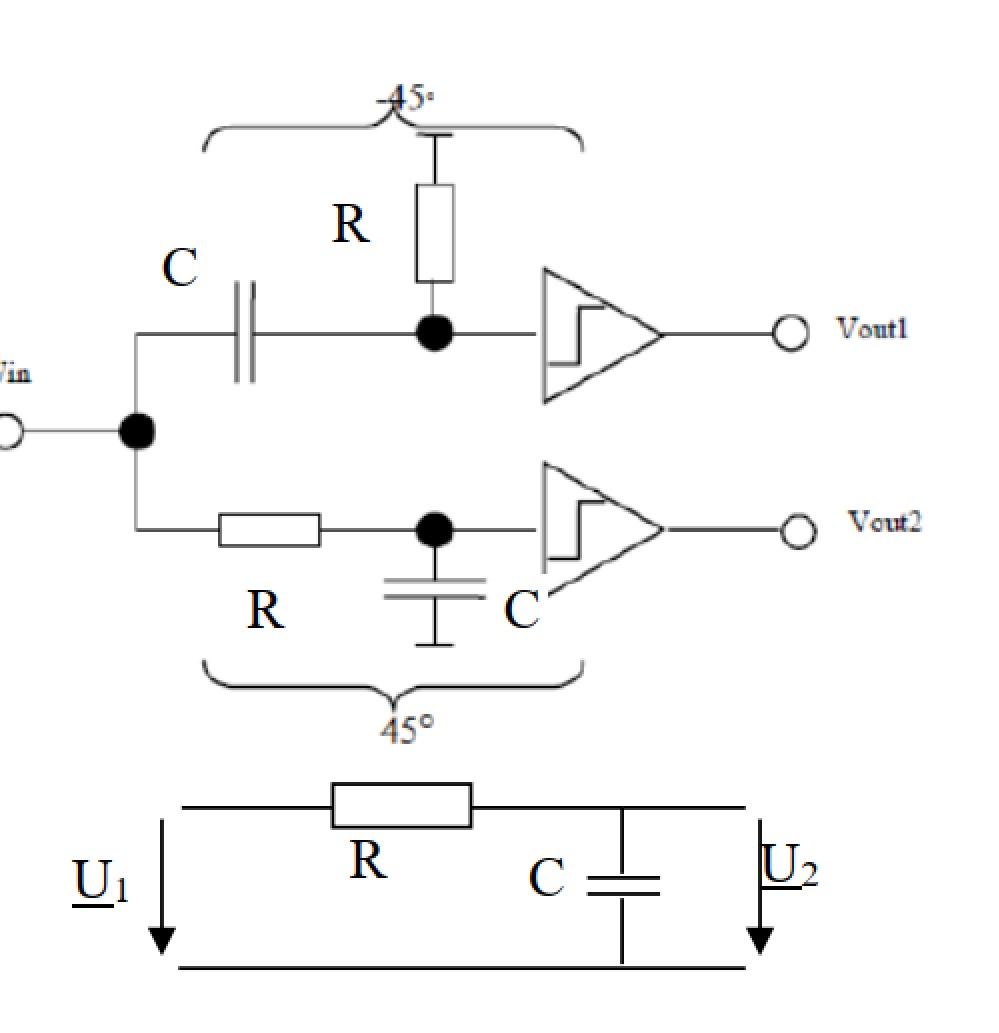
\includegraphics[width=8cm]{images/phase_shifter.jpg}
  \caption{phase shifter}
  \label{fig:phase_shifter}
\end{figure}
\paragraph{DC offset in zero-IF receivers/ self-mixing process}
Assume that the LO power of a zero-IF receiver is given by PLO=0dBm. All impedances are Zo=50
$\Omega$. The isolation between the mixer's LO port and the LNA's input port is 60dB (when connected
at the antenna). The amplification of the combination of LNA and Mixer is 30dB.

Calculate the resulting voltage at the mixer's output. Compare this voltage with the the rms value
of the voltage resulting from an RF signal of -80dBm at the antenna footpoint.\newline\newline
Note: The figure of 30dB isolation between LO and RF port is with connected antenna i.e. the
coupled LO power is divided by 2, one half travelling towards the antenna, the other half travelling
towards the LNA input port.\newline
DC power at mixer's output: (0-30-30+30) dBm = -30 dBm $Rightarrow$ 7mV @ 50$\Omega$
RF power at mixer's output: (-80+30) dBm = -50 dBm $Rightarrow$ 0.7mV rms @ 50$\Omega$\newline
the DC offset voltage is 10x higher as a reasonably strong RF input signal!
\paragraph{Even-order distortion in zero-IF receivers}
Show that zero-IF receivers are susceptible(anfällig) to even-order distortions.\newline\newline
Second order nonlinearity: $y=x^2$\newline
$$
\begin{aligned}
& x(t):=x_1(t)+x_2(t) \\
& x_1(t)=\cos \left(\omega_1 \cdot t\right) \quad x_2(t)=\cos \left(\omega_2 \cdot t\right) \\
& \Rightarrow y(t)=\left[\cos \left(\omega_1 \cdot t\right)+\cos \left(\omega_2 \cdot t\right)\right]^2=\cos ^2\left(\omega_1 \cdot t\right)+\cos ^2\left(\omega_2 \cdot t\right)+2 \cdot \cos \left(\omega_1 \cdot t\right) \cdot \cos \left(\omega_2 \cdot t\right)= \\
& \cos ^2\left(\omega_1 \cdot t\right)+\cos ^2\left(\omega_2 \cdot t\right)+\left\{\cos \left[\left(\omega_1+\omega_2\right) \cdot t\right]+\cos \left[\left(\omega_1-\omega_2\right) \cdot t\right]\right\}
\end{aligned}
$$
If $\omega_1 \approx \omega_2$ then the component $\left(\omega_1-\omega_2\right)$ is a signal near DC, which could interfere with the downconverted wanted signal.
\paragraph{Choice of Receiver Topology}\mbox{}\\
Give some examples how the choice of receiver topology could be influenced by circuit design, economical or other issues. 

\begin{itemize}
    \item Advances in semiconductor technology $\Rightarrow$ higher clock frequencies$\Rightarrow$ possibility to realize certain signal processing functions digitally, which wasn't possible before due to bandwidth limitations, e.g. filtering
    \item Advances of semiconductor technology for computing applications $\Rightarrow$ large volume production $\Rightarrow$ price drop $\Rightarrow$ possibility of application of technology in novel applications for wireless telecommunication systems
\end{itemize}





\paragraph{Superheterodyne Receiver}\mbox{}\\
Discuss the advantage/disadvantage of having the bandpass before and after the amplifier in a superhet receiver with respect to receiver performance:


When the amplifier is before the filter the total noise figure will be improved, but the large signal behaviour becomes worse. Therefore, when one wants high sensitivity the amplifier must be at the beginning, whereas when one wants good large signal behaviour the amplifier must come after the filter.
\paragraph{Superheterodyne Receiver}\mbox{}\\
A receiver has to be designed covering a receiving frequency range between 118...136 MHz.
Determine the lowest possible intermediate frequency in order to be able to remove any image
frequency by an RF filter in front of the mixer stage.
Determine the local oscillator's frequeny range for this case for the two possibilities $f_{RF}<f_{LO}$f and
$f_{RF}<F_{LO}$f. Considering the result of b), which problem arises if an IF near the minimum IF is used? What would be the minimum value of the IF to circumvent the problem in c)? Discuss advantages and disadvantages to select the LO frequency above or below the receiving frequency\newline\newline
\begin{enumerate}
    \item From \autoref{eq:image_frequency} we know that $f_{I M}=f_{R F} \pm 2 f_{I F}$. Furthermore, one can see from \autoref{fig:image_freq_1} that $f_{I F}$ must at least be $\frac{1}{2}$ of the bandwidth of the signal which is $f_{I F} > \frac{1}{2}\cdot (f_{RF_{max}}-f_{RF_{max}})=9MHz$.
    \item According to \autoref{eq:mixer_output} $f_{I F}=\left|f_{R F} \pm f_{L O}\right|$ furthermore, the sign is minus for the case where $f_{L F}<f_{R F}$ due to that and the fact that $f_{R F}-f_{L F}=9MHz$ must always be true $f_{L F}$ has a range from 109-127MHz. For the case where $f_{L F}>f_{R F}$ the sign is opposite and therefore in the range 127MHz-145MHz.
    \item 
    \begin{itemize}
        \item The leakage from LO to RF port (typically in the order of -30dB) may be partially reflected at the antenna port and then self-mixed with the LO signal. This results in a DC component in the downconverted signal. As long as the receiver topology is an IF topology, this DC component can be removed by high pass or band pass filtering. However, if the receiver topology is a zero-IF topology, then it is difficult if not impossible to remove this offset.
        \item Moreover, the LO leakage signal passes the RF input filter backwards and may be reradiated by the receiving antenna. To avoid this re-radiation, the LO frequency range must be placed out of the receiving frequency range $\Rightarrow$ possibility to reject backwards path by the RF bandpass
    \end{itemize}
    \item To avoid the second problem in c):
    $$
    \begin{aligned}
    \text { Aussuming } f_{\mathrm{LO}}<f_{\mathrm{RF}} & \Rightarrow f_{\mathrm{LO}, \max }<f_{\mathrm{RF}, \min } \\
    & f_{\mathrm{RF}, \max }-f_{\mathrm{IF}}<f_{\mathrm{RF}, \min } \\
    & f_{\mathrm{IF}}>f_{\mathrm{RF}, \max }-f_{\mathrm{RF}, \min }=18 \mathrm{MHz}
    \end{aligned}
    $$
    \item $\mathrm{f}_{\mathrm{LO}}<\mathrm{f}_{\mathrm{RF}}$\newline
    Advantages:
    \begin{itemize}
        \item lower frequency range
        \item spectrum at IF is not inverted
    \end{itemize}
    \textbf{Disadvantages:}
    \begin{itemize}
        \item bigger relative bandwidth
    \end{itemize}
    $f_{L O}>f_{R F}$ vice versa
\end{enumerate}





\paragraph{Dual-IF topology with image-signal rejection}\mbox{}\\
A given dual-IF topology (see above figure) has the following specifications:\newline
$f_{R F}$ = 87.5MHz...108 MHz\newline
Bandwidth of the received signal: B=180kHz\newline
First IF at $f_{IF_1}$=10.7 MHz\newline
Second IF at $f_{IF_2}$=455 kHz\newline
$f_{LO_1}<f_{RF}$\newline
Determine all spurious signals which could occur due to the selection of this set of intermediate
frequencies if the RF input frequency is given by $f_{R F}$ = 90.7 MHz.
Why is Filter 2 in \autoref{fig:double_superheterodyne_receiver} needed?
What is the maximum bandwidth of Filter 2 in \autoref{fig:double_superheterodyne_receiver} to fulfil its function (see b))?

\begin{enumerate}
    \item 
    \begin{itemize}
        \item $f_{\mathrm{LO} 1}=\mathrm{f}_{\mathrm{RF}}-\mathrm{f}_{\mathrm{IF} 1}=90.7 \mathrm{MHz}-10.7 \mathrm{MHz}=80 \mathrm{MHz}$
        \item 2 possible cases for $f_{\mathrm{LO2}}$ :
        \begin{itemize}
            \item $f_{\mathrm{LO2}}<f_{\mathrm{IF} 1}:  f_{\mathrm{LO2}}=\mathrm{f}_{\mathrm{IF} 1}-\mathrm{f}_{\mathrm{IF} 2}=10.7 \mathrm{MHz}-0.455 \mathrm{MHz}=10.245 \mathrm{MHz}$
            \item $f_{\mathrm{LO2}}>\mathrm{f}_{\mathrm{IF} 1}:  \mathrm{f}_{\mathrm{LO2}}=\mathrm{f}_{\mathrm{IF} 1}+\mathrm{f}_{\mathrm{IF} 2}=10.7 \mathrm{MHz}+0.455 \mathrm{MHz}=11.155 \mathrm{MHz}$
        \end{itemize}
        \item Other mixing products
        $$\begin{aligned} \mathrm{f}_{\mathrm{IF} 1}^{\prime} & =\mathrm{f}_{\mathrm{RF}}+\mathrm{f}_{\mathrm{LO} 1}=90.7 \mathrm{MHz}+80 \mathrm{MHz}=170.7 \mathrm{MHz} \\ & \Rightarrow \text { Has to be rejected by } \mathrm{BPF}_{3} ! \\ \mathrm{f}_{\mathrm{IF2} 2}^{\prime} & =\mathrm{f}_{\mathrm{IF} 1}+\mathrm{f}_{\mathrm{LO2}}=10.7 \mathrm{MHz}+10.245 \mathrm{MHz}=20.945 \mathrm{MHz}\left(\text { if } \mathrm{f}_{\mathrm{LO2}}<\mathrm{f}_{\mathrm{IF} 1}\right) \\ \mathrm{f}_{\mathrm{IF} 2}^{\prime} & =\mathrm{f}_{\mathrm{IF} 1}+\mathrm{f}_{\mathrm{LO2}}=10.7 \mathrm{MHz}+11.155 \mathrm{MHz}=21.855 \mathrm{MHz}\left(\text { if } \mathrm{f}_{\mathrm{LO2}}>\mathrm{f}_{\mathrm{IF} 1}\right)\end{aligned}$$
    \end{itemize}
    \item Need of Filter 2
    \begin{itemize}
        \item To reject other than the wanted mixing product of mixer 1
        \item To work as an image-reject filter for the second mixer stage
    \end{itemize}
    \item The situation can be seen in \autoref{fig:image_ex_1} and \autoref{fig:image_ex_2}. Filter 2 in \autoref{fig:double_superheterodyne_receiver} must therefore at least block the image frequencies, when $f_{LO_{2,2}}$ is chosen it must block at least all frequencies that are higher than 9.79MHz+0.09MHz=9.88MHz
    
\end{enumerate}
\begin{figure}[ht]
  \centering
  \resizebox{1\textwidth}{!}{\subimport{images/}{spectrum_1.tex}}
  \caption{Image frequencies with bandpass}
  \label{fig:image_ex_1}
\end{figure}

\begin{figure}[ht]
  \centering
  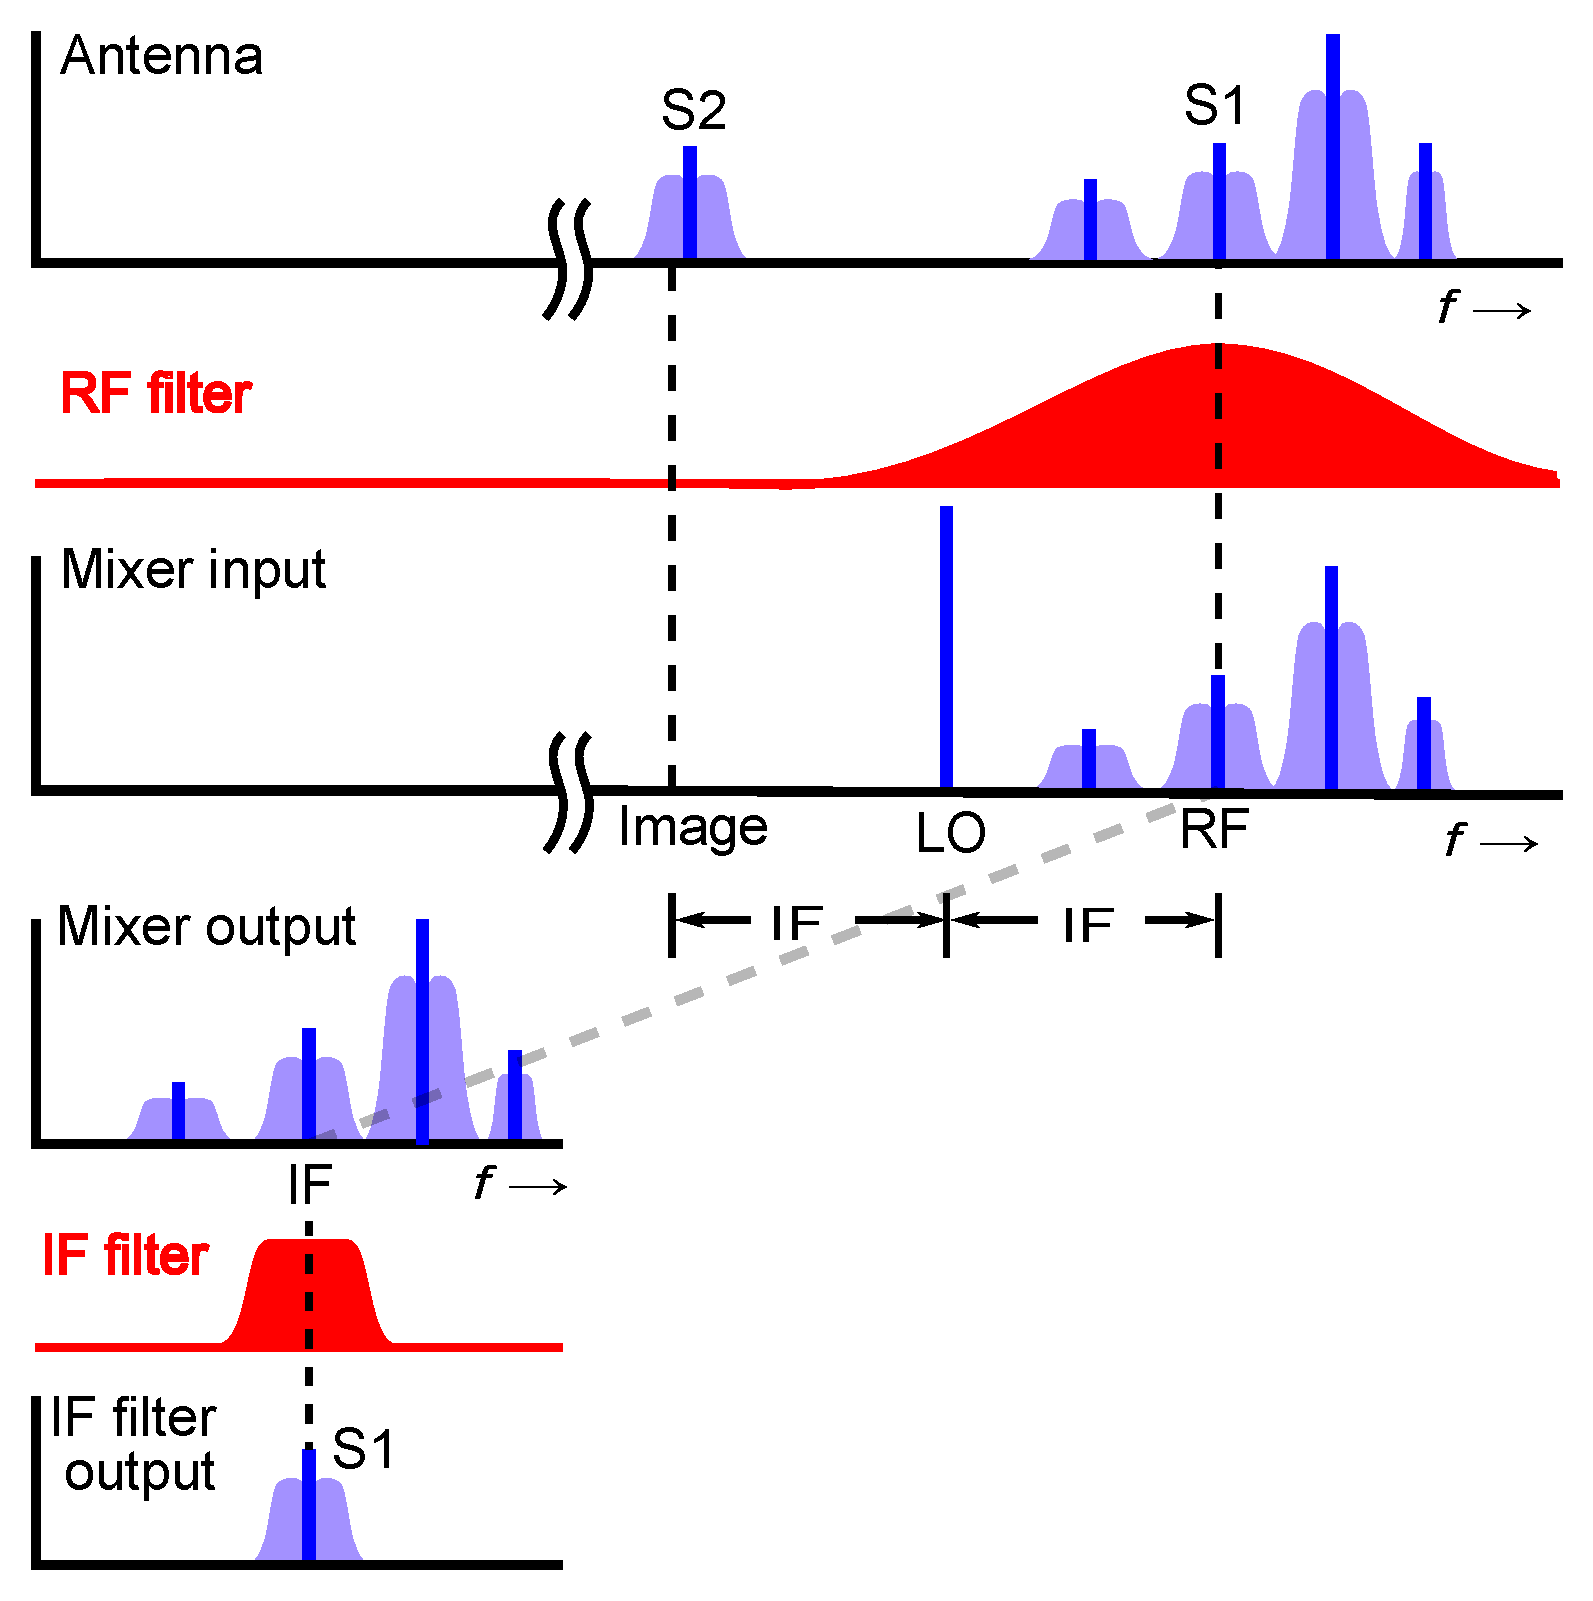
\includegraphics[width=8cm]{images/Superheterodyne2.pdf}
  \caption{superheterodyne radio principle}
  \label{fig:typical_superheterodyne_receiver_principle}
\end{figure}
\begin{figure}[ht]
  \centering
  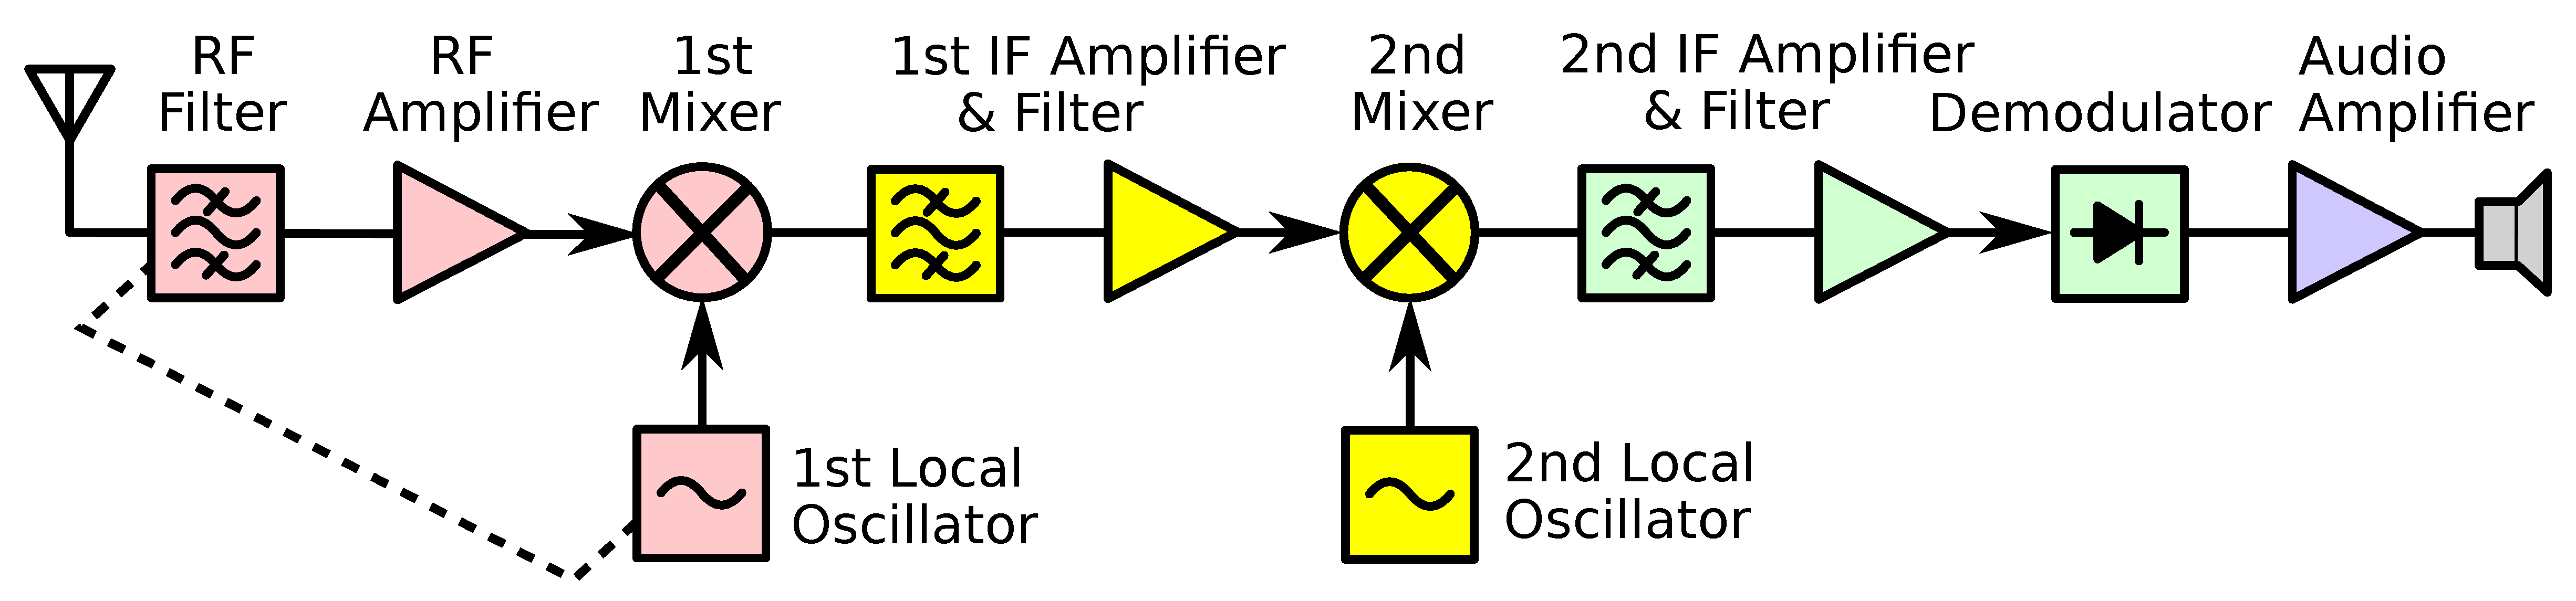
\includegraphics[width=8cm]{images/Superheterodyne3.pdf}
  \caption{Double conversion superheterodyne receiver block diagram}
  \label{fig:double_superheterodyne_receiver}
\end{figure}



\begin{figure}[ht]
  \centering
  \resizebox{1\textwidth}{!}{\subimport{images/}{spectrum_2.tex}}
  \caption{Image frequencies with bandpass}
  \label{fig:image_ex_2}
\end{figure}
\begin{figure}[ht]
  \centering
  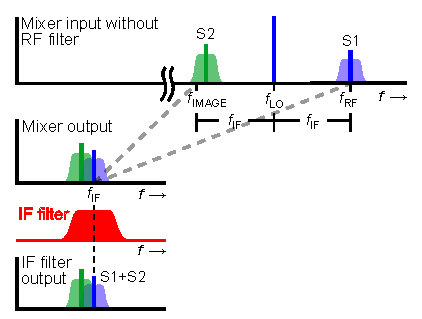
\includegraphics[width=8cm]{images/Superheterodyne4.pdf}
  \caption{illustrating for the problem of image response}
  \label{fig:image_response}
\end{figure}
\section{Receiver}
Designing sharp filters for high frequencies in CMOS technology, which is often used, is quite difficult. Due to that one came up with different receiver technologies to be able to implement those filters at lower frequencies. To do that one ore more local oscillators are needed which consume quite a lot of energy. Therefore nowadays, one tries to prevent having local oscillators when possible. Nevertheless, it was often used and is still used in some applications. Therefore one has a look at them in this chapter.
\subsection{Conversion to baseband}
Problem is that when signal is not symmetric it is not working. A solution would be to multiplie it with a complex signal.
\begin{equation}
\underline{\mathrm{x}}(\mathrm{t})=\mathrm{e}^{-\mathrm{j} \omega \mathrm{ct}}=\cos \left(\omega_{\mathrm{c}} \mathrm{t}\right)-\mathrm{j} \cdot \sin \left(\omega_{\mathrm{c}} \mathrm{t}\right)=\cos \left(\omega_{\mathrm{c}} \mathrm{t}\right)+\mathrm{j} \cdot \cos \left(\omega_{\mathrm{c}} \mathrm{t}-90^{\circ}\right)
\end{equation}
This is the idea of the zero-if approach. The issue is when one has a little phase shift then one gets some image. One issue of this approach is the dc offset.
When something is near the antenna the antenna has a different impedance. From the mixer some signal goes to the antenna with the $\omega_{LO}$ frequency. When the antenna is not matched the signal comes back the amount of the signal that comes back is dependent on the environment. Today one solves this problem by leaving always the carrier in the middle at the frequency of zero.
\subsection{Low-IF receiver}
\subsection{Hartley-Architecture}
It is difficult to have a 90 degree phase shift for a whole frequency band.
The image rejection ratio can be callculated with \autoref{eq:image_rejection_ratio} where the variables mean the following:\newline
$\delta G=a m p l i t u d e ~ e r r o r$\newline
$\delta \varphi=$ phase error\newline
\begin{equation}\label{eq:image_rejection_ratio}
I R R=\sqrt{\sin ^2\left(\frac{\delta \varphi}{2}\right)+\left(\frac{\delta G}{2 G}\right)^2 \cdot \cos ^2\left(\frac{\delta \varphi}{2}\right)}
\end{equation}

\subsubsection{Dual-IF Receiver with image rejection}


\section{Considerations for Bandpass Sampling Architectures}
An analog bandpass signal x(t) can be fully reconstructed if it's sampled with a frequency of more than two times the bandwidth of x(t)

Sampled signal
$$
\text { Sampled signal } \quad x_a(t)=x(t) \cdot \sum_{n=-\infty}^{\infty} \delta(t-n T)
$$
$$
\text { Spectrum of the sampled signal } \quad X_a(f)=X(f) *\left[\frac{1}{T} \sum_{n=-\infty}^{\infty} \delta\left(f-\frac{n}{T}\right)\right]
$$

$$
\begin{array}{rlrl} 
& -f_u+k \cdot f_A<f_u & & \frac{2 \cdot f_u}{k}>f_A>\frac{2 \cdot f_O}{k+1} \\
-f_o+(k+1) \cdot f_A>f_o & & \\
& (k+1) \cdot f_u & >k \cdot f_o & 0 \leq k<\frac{f_u}{B} \\
k \cdot f_u+f_u & >k \cdot f_o & & \\
k \cdot\left(f_o-f_u\right) & =k \cdot B<f_u & &
\end{array}
$$
The idea is to get a digital downconversion instead of a analog one, due to sampling theorem.
The problem is that one has mirror from the left side, therefore it would be nice if one can remove it.
Analytic signal has only positive frequency components, is not anymore a real time signal, since a real signal has always a positive and negative part.
\section{Wave propagation}
The frequency response of the channel is given by H(t).
\begin{equation}
\underline{H}(f, t)=\frac{\underline{Y}(f, t)}{\underline{X}(f, t)}
\end{equation}
Important wave progpagations modes
\begin{itemize}
    \item Ground wave propagation\newline
    Wave is conducted by the earths surface (air and earth). The issue with this path is that one has losses (currents in the earth that have a resistance). The higher the frequency the larger the losses get.
    \item Sky wave propagation, we have positively and negatively charger particles in the ionosphere which act as a conductor.
    \item Line of sight (LOS)
\end{itemize}
\subsection{Exercise 13}
\begin{itemize}
    \item \textbf{Image Reject Mixers: Calculate the image rejection ratio at a given phase error of 3$^\circ$ and an amplitude error of 2 dB}\newline
    According to \autoref{eq:image_rejection_ratio} the following holds:
    $$
    I R R^h=\sqrt{\sin ^2\left(\frac{\delta \varphi}{2}\right)+\left(\frac{\delta G}{2 G}\right)^2 \cdot \cos ^2\left(\frac{\delta \varphi}{2}\right)}
    $$
    where $\delta G$ = amplitude error and $\delta \varphi$ = phase error, therefore $\frac{\delta G}{G}=10^{\frac{2}{20}}-1$ = 0.259.
     $$
    I R R^h=\sqrt{\sin ^2\left(\frac{3^{\circ}}{2}\right)+\left(\frac{10^{\frac{2}{20}}-1}{2}\right)^2 \cdot \cos ^2\left(\frac{3^{\circ}}{2}\right)}=17.586dB
    $$
\end{itemize}



%https://github.com/l3v5y/UW-Electronics-Lecture-Notes/blob/master/ES335%20-%20Communication%20Systems.tex
% \begin{figure}[h]
%     \begin{tikzpicture}
%         \draw[->] (1,0) node [below]{$(f_0-f_m)$} -- (1,1) node [above left] {$(\frac{A_0m}{2})$};
%         \draw[->] (7,0) node [below]{$(f_0+f_m)$} -- (7,1) node [above right] {$(\frac{A_0m}{2})$};
%         \draw[->] (4,0) node [below]{$f_0$} -- (4,2) node [above right] {$A_0$};
%         \draw[->] (0,0) -> (8,0) node [below right] {$f(\omega )$};
%         \draw[<->] (1,0.5)--(4,0.5);
%         \node[align=center, above] at (2.5,0.5) {$f_m(\omega_m)$};
%         \node[align=center, above] at (5.5,0.5) {$f_m(\omega_m)$};
%         \draw[<->] (7,0.5)--(4,0.5);
%     \end{tikzpicture}
%     \centering
%     \caption{Spectrum of an AM signal, including sidebands}
% \end{figure}
\section{Propagation models}
The calculation of the power density $S_R$ at the receiver at a given distance d can be done according to \autoref{eq:power_density}, where P is the power and $G_T$ the antenna gain.
\begin{equation}\label{eq:power_density}
    S_R=\frac{P \cdot G_T}{4 \pi d^2}
\end{equation}
The pointing vector can be calculated according to \autoref{eq:pointing_vector}
\begin{equation}\label{eq:pointing_vector}
    \vec{S}=\vec{E} \times \vec{H}
\end{equation}
The field wave impedance can be calculated according to \autoref{eq:field wave impedance}
\begin{equation}\label{eq:field wave impedance}
    Z_f=\frac{E}{H}=120 \pi \approx 377[\Omega]
\end{equation}
The Electrical field strength (rms) can be calculated according to \autoref{eq:electrical_filed_strength}, which as the combination of \autoref{eq:field wave impedance}, \autoref{eq:pointing_vector} and \autoref{eq:power_density}.
\begin{equation}\label{eq:electrical_filed_strength}
E=\sqrt{\frac{P \cdot G_T \cdot Z_f}{4 \pi d^2}}
\end{equation}
The equivalent absorption area of a receiving antenna is given by \autoref{eq:equivalen_absorption}
\begin{equation}\label{eq:equivalen_absorption}
    A_R=G_R \cdot \frac{\lambda^2}{4 \pi}
\end{equation}
\begin{equation}
P_R=\frac{P_T \cdot G_T \cdot G_R}{(4 \pi \cdot d / \lambda)^2}
\end{equation}
\autoref{eq:free_space_loss} Shows the free space loss:
\begin{equation}\label{eq:free_space_loss}
A_F=(4 \pi \cdot d / \lambda)^2
\end{equation}
Where $\lambda=\frac{\mathrm{V}}{\mathrm{f}}$.
\subsubsection{Wave propagation model by Okumura-Hata}
\begin{equation}\label{eq:okumura-hata}
L_{H u}[d B]=69.55+26.16 \cdot \log \frac{f}{M H z}-13.82 \cdot \log \frac{h_{B S}}{m}-a\left(h_{M S}\right)+\left(44.9-6.55 \log \frac{h_{B S}}{m}\right) \cdot \log \frac{d}{k m}
\end{equation}
\begin{itemize}
    \item Transmit frequency: $f$
    \item Height of base station antenna: $h_{BS}$
    \item Height of mobile station antenna: $h_{MS}$
    \item Distance: $d$
\end{itemize}
Correction terms
\begin{itemize}
    \item Correction term for small and medium-sized cities:
    $$
    a\left(h_{M S}\right)=\left(1.1 \cdot \log \frac{f}{M H z}-0.7\right) \cdot \frac{h_{M S}}{m}-\left(1.56 \cdot \log \frac{f}{M H z}-0.8\right)
    $$
    \item Correction term for metropolises:
    $$
    a\left(h_{M S}\right)= \begin{cases}8.29 \cdot\left[\log \left(1.54 \cdot \frac{h_{M S}}{m}\right)\right]_2^2-1.1 & f \leqslant 200 \mathrm{MHz} \\ 3.2 \cdot\left[\log \left(11.75 \cdot \frac{h_{M S}}{m}\right)\right]^2-4.97 & f \geqslant 400 \mathrm{MHz}\end{cases}
    $$
    \item Correction term for sub-urban areas:
    $$
    L_{H s}[d B]=L_{H u}-2 \cdot\left[\log \frac{f}{28 \mathrm{MHz}}\right]^2-5.4
    $$
    \item Correction term for rural areas:
    $$
    L_{H r}[d B]=L_{H u}-4.78 \cdot\left[ \log \frac{f}{M H z}\right]^2+18.33 \cdot \log \frac{f}{M H z}-40.94
    $$
\end{itemize}




\subsubsection{Air refraction effects}
Due to variations of air temperature/pressure/humidity, the refraction index varies with height above ground.
\subsubsection{Important radio channel effects in mobile communicaionts}
$$
\begin{array}{|c|c|}
\hline \text { Type/Reason } & \text { Effect } \\
\hline \text { Multipath } & \text { Fast Fading } \\
& \text { Delay Spread (Zeitdispersion) } \\
\hline \text { Movement } & \text { Doppler Shift } \\
& \text { Frequency Dispersion } \\
\hline \text { Shadowing effect } & \text { Slow Fading } \\
\hline \text { Path losses } & \text { Signal attenuation } \\
\hline
\end{array}
$$
The Doppler frequency is described with \autoref{eq:doppler_frequency}
\begin{equation}\label{eq:doppler_frequency}
f_D=\frac{1}{2 \pi} \frac{d \varphi}{d t}=f_m \sin \alpha
\end{equation}
The maximum Doppler frequency $f_m$ is given by 
\begin{equation}
f_m=\frac{v}{\lambda}=\frac{v}{c \cdot f}
\end{equation}

\subsubsection{coherence time and coherence bandwidth}
\begin{itemize}
    \item Coherence Time: measure for the time period in which the channel properties remain approximately constant.
    \begin{equation}\label{eq:corherence_time}
    \mathrm{T}_{\mathrm{tc}}=1 / \mathrm{B_d}
    \end{equation}
    $B_d$ = Doppler spread bandwidth
    \item Coherence bandwidth: measure for the bandwidth, in which the channel properties remain highly correlated.
    \begin{equation}\label{eq:coherence_bandwidth}
    \mathrm{B}_{\mathrm{cb}}=1 / \mathrm{T_m}
    \end{equation}
    $T_m$ = delay spread \newline
    $\Rightarrow$ all frequency component within $B_{cb}$ will be almost equally attenuated.
\end{itemize}

\paragraph{Two-ray-model}
A base station transceiver transmits a GSM signal on a channel within the frequency range of f = 935,2MHz...935.4MHz. A mobile station (MS) is connected to this base station (BS). Let us assume that there is a line-of sight condition between them. Imagine further that there is a mountain chain parallel to the line-of-sight connection at a distance of h=2km, which partially reflects incident radio signals.
Let us assume further:
\begin{enumerate}
    \item The mountain chain is modelled as a vertical wall (see figure below).
    \item The antennas of both the BS and the MS have an omnidirectional radiation pattern in the horizontal plane
    \item The radio signal propagates from the BS to the MS by just two paths, namely the direct path (i.e. line-of-sight), and one reflected path, by reflection at the vertical wall. (Any further reflections such as ground reflection shall be neglected).
    \item The reflection itself obeys the principles of geometrical optics.
    \item The attenuation of the receiving field strength due to the detour of the reflected path is neglected, or considered to be already included in the reflection coefficient \textcolor{orange}{r}.
    \item Distance between BS and MS: d = 5km
    \item Reflection coefficient at the wall for the E field under the given incident angle: r = 0.5 (real)
\end{enumerate}
\begin{itemize}
    \item \textbf{Determine the radio channel's amplitude response between the BS and the MS for the given GSM-channel (i.e. between 935,2 MHz ... 935,4 MHz)}\newline
    According to \autoref{eq:superimposed_complex_signal} the following holds:
    $$
    \underline{g}(\vec{y})=\sum_{n=0}^{N-1} \underline{w}_n \cdot g_n(\phi) \cdot \exp \left(-\mathrm{j} \cdot \mathrm{k}\left|\overrightarrow{x_n}-\vec{y}\right|\right)
    $$
    Due to that the received signal is
    $$y_1(t)=w_t \cdot \boldsymbol{e}^{i\cdot \frac{2 \cdot \pi}{\frac{\SI{3e8}{\meter\per\second}}{f_{RF}}}\cdot \SI{5000}{\meter}}$$ and $$y_2(t)=\textcolor{orange}{0.5} \cdot w_t \cdot \boldsymbol{e}^{i\cdot \frac{2 \cdot \pi}{\frac{\SI{3e8}{\meter\per\second}}{f_{RF}}}\cdot \sqrt{(\SI{2500}{\meter})^2+(\SI{2000}{\meter})^2}\cdot2}$$ 
    $$
    \left| w_t \cdot \boldsymbol{e}^{i\cdot \frac{2 \cdot \pi}{\frac{\SI{3e8}{\meter\per\second}}{f_{RF}}}\cdot \SI{5000}{\meter}}  +\textcolor{orange}{0.5} \cdot w_t \cdot \boldsymbol{e}^{i\cdot \frac{2 \cdot \pi}{\frac{\SI{3e8}{\meter\per\second}}{f_{RF}}}\cdot \sqrt{(\SI{2500}{\meter})^2+(\SI{2000}{\meter})^2}\cdot2}  \right|
    $$
    And the Amplitude spectrum of the graph in the range from 935,2MHz...935.4MHz looks like in \autoref{fig:graph_ploted}
    \begin{figure}[ht]
      \centering
      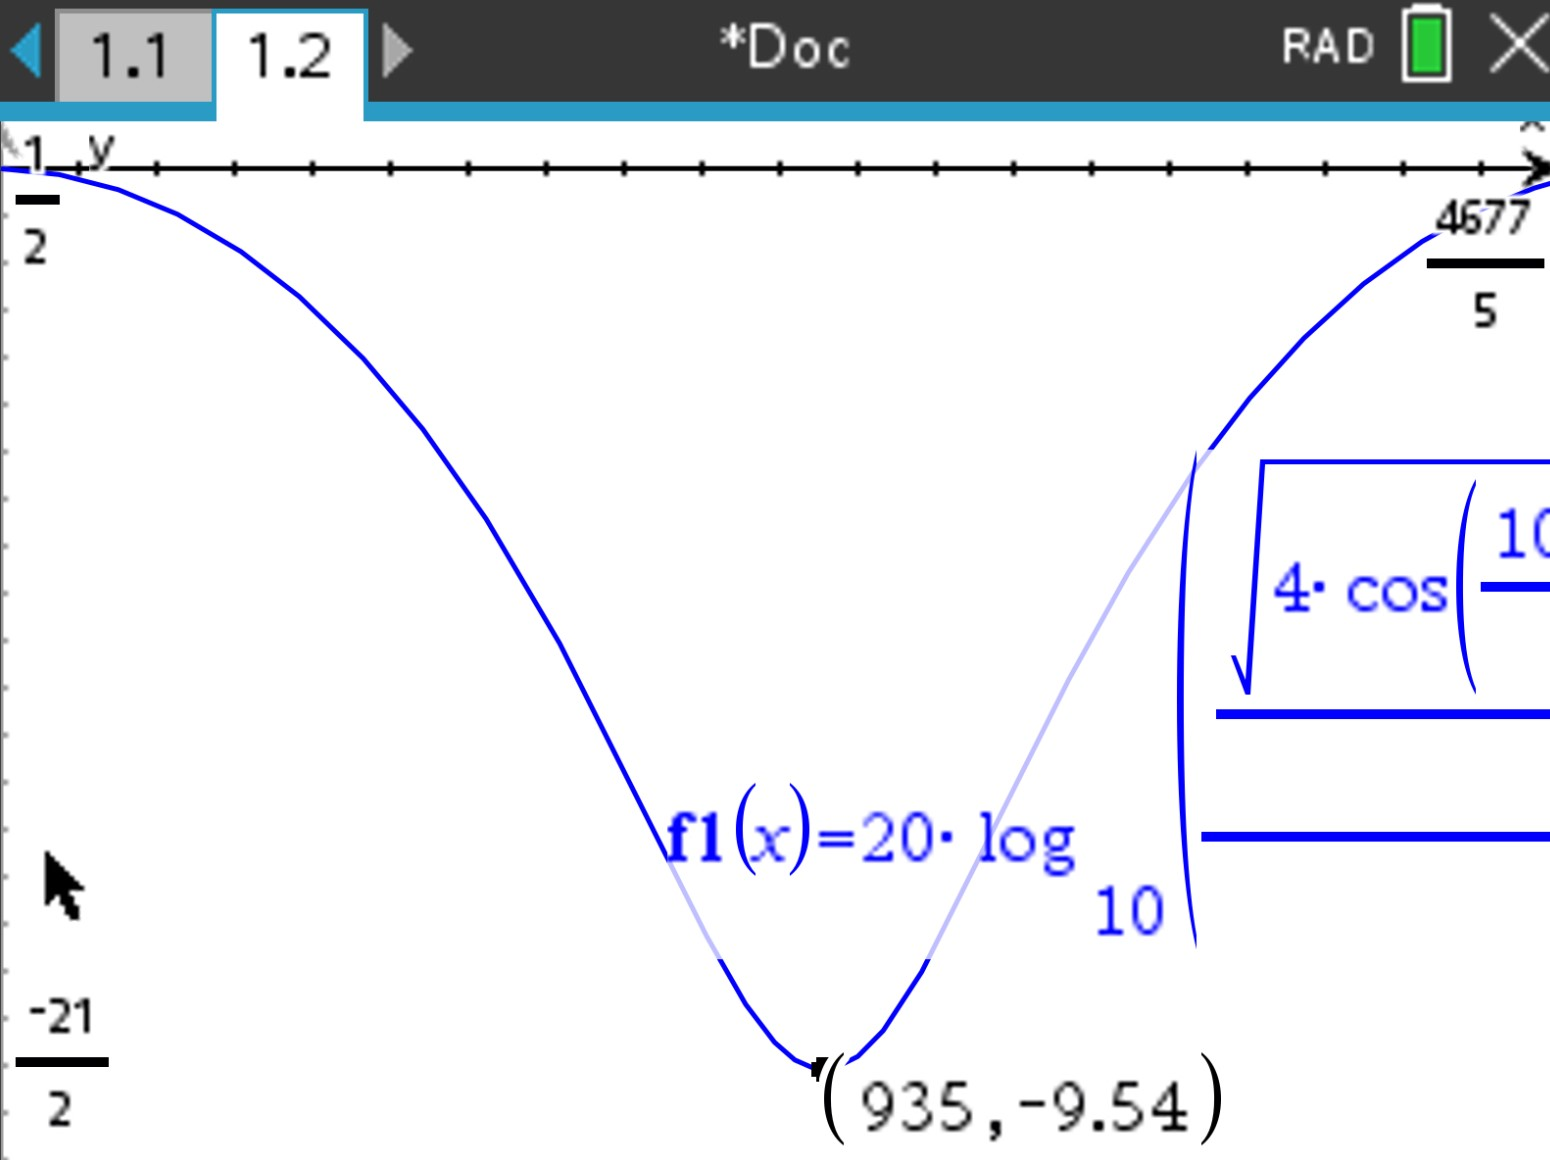
\includegraphics[width=8cm]{images/graph.jpg}
      \caption{plotted graph form exercise}
      \label{fig:graph_ploted}
    \end{figure}
    \item \textbf{Assuming that the radio channel's allowed tolerance of the amplitude response is given by 3dB. Is the radio channel frequency-selective?}\newline
    The radio channel's amplitude response varies up to approximately 10 db as it can also be seen in \autoref{fig:graph_ploted} and is therefore frequency-selective.
    \item \textbf{How will $|\underline{H}(\mathrm{f})|$ change, if the reflection coefficient is changed from 0.5 to 0.8?} \newline
    The reflected path has an increased amplitude. If it is dephased by 180 degrees, the amplitude of the total received signal is more attenuated. Therefore, stronger variations are expected.
    \item\textbf{ In the last example, ' $\textcolor{orange}{r}$ ' was real valued. This is not necessarily the case. How will $|\underline{H}(\mathrm{f})|$ change if the reflection coefficient is given by $\underline{r}_1=0.8 \angle 60^{\circ}$ ?}\newline
    The relative phase relation between direct path and reflected path has been changed. Therefore, the 180 degree out-of-phase occurs at an other frequency. (spectrum is shifted)
    \item \textbf{Consider qualitatively how $|\underline{H}(\mathrm{f})|$ will be changed, if the distance to the mountain chain becomes bigger.}\newline
    The bigger the distance to the mountain, the bigger is the detour $\Delta$. As easily can be seen form the formula for y(f). The relative phase change at a given frequency change is proportional to the detour $\Delta$. It is therefore expected that the amplitude variations with respect to the frequency chances will become faster.
    \item \textbf{The distance to the mountain wall is now given by $h_1$=700m, the reflection coefficient is r=0.5 (real). Is the radio channel-as defined in b) -frequency-selective?}\newline
    No the variations are only about 0.5dB. Since we are closer to the mountain, the periodicity of the channel is lower, as described before.

\end{itemize}
\paragraph{Free-space attenuation}
\begin{itemize}
    \item \textbf{Calculate the free-space attenuation at between two locations at a distance of d= 5km, if the frequency is 900 MHz?}\newline
    According to \autoref{eq:free_space_loss} which says $A_F=(4 \pi \cdot d / \lambda)^2$ one gets $A_F=(4 \pi \cdot \SI{5000}{\meter} / \frac{\SI{3e8}{\meter\per\second}}{\SI{900e6}{\per\second}})^2=\SI{35.53e9}{}$ and in dB: $10\log_{10}(\SI{35.53e9}{})=\SI{105.512}{}$dB
    \item \textbf{What is the rms value of the electrical field at the receiver, if the transmitting power is P=500 W EIRP?}\newline
    According to \autoref{eq:electrical_filed_strength} the following holds $E=\sqrt{\frac{P \cdot G_T \cdot Z_f}{4 \pi d^2}}=\sqrt{\frac{\SI{500}{\watt} \cdot 1 \cdot \SI{377}{\ohm}}{4 \pi (\SI{5000}{\meter})^2}}=\SI{24.4949e-3}{\volt\per\meter}$
\end{itemize}

\paragraph{Okumura-Hata model}
\begin{itemize}
    \item\textbf{ Determine the path loss in urban environment using the Okumura-Hata model for the following scenario:}
    \begin{itemize}
        \item Height of transmitting antenna: $h_t$ = 50m
        \item Height of receiving antenna: $h_r$ = 1.5m
        \item Frequency: f= 900MHz
        \item Distance between transmitter and receiver: d = 5km
        \item Big city
    \end{itemize}
    According to \autoref{eq:okumura-hata} one knows that 
    $$
    \begin{aligned}
    L_{H u}[d B]&=69.55+26.16 \cdot \log \frac{f}{M H z}-13.82 \cdot \log \frac{h_{B S}}{m}-\underbrace{a\left(h_{M S}\right)}_{\text{0 for urban}}+\left(44.9-6.55 \log \frac{h_{B S}}{m}\right) \cdot \log \frac{d}{k m}\\
    &=69.55+26.16 \cdot \log(900) -13.82 \cdot \log(\SI{50}{\meter})+\left(44.9-6.55 \log(\SI{50}{\meter})\right) \cdot \log 5\\&=\underline{\underline{146.959dB}}
    \end{aligned}
    $$
    \item Same scenario, but for rural environment
    $$
    L_{H r}[d B]=146.959dB -4.78 \cdot\left[ \log(900)\right]^2+18.33 \cdot \log(900)-40.94=\underline{\underline{118.452dB}}
    $$
    
    \item Compare the results with result of Problem 2 a)
\end{itemize}
\paragraph{Time-variant channel modelling I}
\begin{itemize}
    \item \textbf{Derive a channel model for a ionospheric 2-path propagation, if the relative time shift between the two signal paths is 1ms whereas the signal bandwidth is 10 kHz.}\newline
    Time resolution is $\frac{1}{W}=\frac{1}{\SI{10}{\kilo\hertz}}=\SI{0.1}{\milli\second}$. ==> The delay line model consists of 10 taps where only the first and the last have (time-varying coefficients)
    \item \textbf{Determine the coherence bandwidth}\newline
    % According to \autoref{eq:corherence_time} the following holds: $\mathrm{T}_{\mathrm{tc}}=1 / \mathrm{B_d}=\frac{1}{}$
    According to \autoref{eq:coherence_bandwidth} the following holds: $\mathrm{B}_{\mathrm{cb}}=1 / \mathrm{T_m}=\frac{1}{\SI{1}{\milli\second}}=\SI{1000}{\hertz}$. Within this bandwidth all frequency components of a signal are modified in a similar way, e.g. all frequency components within $B_c$ could be simultaneously attenuated.
\end{itemize}

\paragraph{Time-variant channel modelling II}
\begin{itemize}
    \item \textbf{Determine a channel model for a communication link between two aircrafts if there is a direct path and a second path resulting from scattering at the earth surface. The scattered path has a delay of $\tau=\SI{10e-6}{\second}$. The signal bandwidth is W=100 kHz.}
    
    \item \textbf{Same scenario, but with a signal bandwidth of W=10kHz}
\end{itemize}


Exam: Bring laptop with to the exam, submission is online, when we write on papaer, we have to scan in programms on the computer are not allowed but local pdfs are.
\section{Formulas}
\subsection{Probability}
\subsubsection{Q-funciton}
\begin{equation}\label{q-funciton}
Q(x)=\frac{1}{\sqrt{2 \pi}} \int_x^{\infty} \exp \left(-\frac{u^2}{2}\right) d u
\end{equation}
\subsubsection{Binomialverteilung}
Ein Bernoulli-Experiment mit den beiden sich gegenseitig ausschliessenden Ergebnissen (Ereignissen) $A$ und $\bar{A}$ werde $n$-mal nacheinander ausgefuehrt (sog. mehrstufiges Bernoulli-Experiment vom Umfang $n$ ). Dann genuegt die diskrete Zufallsvariable
$$
    \text{$X=$ Anzahl der Versuche, in denen das Ereignis A eintritt}
$$
der sog. Binomialverteilung mit der Wahrscheinlichkeitsfunktion
\begin{equation}\label{eq:binomial_function}
    f(x)=P(X=x)=\left(\begin{array}{c}
    n \\
    x
    \end{array}\right) p^x \cdot q^{n-x} \quad(x=0,1,2, \ldots, n)
\end{equation}

und der zugehoerigen Verteilungsfunktion
$$
F(x)=P(X \leq x)=\sum_{k \leq x}\left(\begin{array}{l}
n \\
k
\end{array}\right) p^k \cdot q^{n-k} \quad(x \geq 0)
$$
(fuer $x<0$ ist $F(x)=0$ ). $n$ und $p$ sind dabei die Parameter der Verteilung. Die Kennwerte oder Masszahlen der Binomialverteilung lauten:
\begin{itemize}
    \item Mittelwert: $\mu=n p$
    \item Varianz: $\quad \sigma^2=n p q=n p(1-p)$
    \item Standardabweichung: $\sigma=\sqrt{n p q}=\sqrt{n p(1-p)}$
\end{itemize}
Dabei bedeuten:
\begin{itemize}
    \item p: Konstante Wahrscheinlichkeit für das Eintreten des Ereignisses A beim Einzelversuch $(0<p<1)$
    \item $q$ : Konstante Wahrscheinlichkeit für das Eintreten des zu A komplementären Ereignisses $\bar{A}$ beim Einzelversuch $(q=1-p)$
    \item $n$ : Anzahl der Ausführungen des Bernoulli-Experiments (Umfang des mehrstufigen Bernoulli-Experiments)
\end{itemize}

\section*{Common angles}


\begin{table}[!ht]
\setlength{\tabcolsep}{1em} % Increase the horizontal table cell margin
\centering
  \tabulinesep=1.5mm
  \begin{tabu}{|c|c|c|c|c|c|c|c|}
    \hline
    \textbf{Degrees}
      & $\SI{0}{\degree}$
      & $\SI{30}{\degree}$
      & $\SI{45}{\degree}$
      & $\SI{60}{\degree}$
      & $\SI{90}{\degree}$\\
    \hline
    \textbf{Radians}
      & $\displaystyle 0$
      & $\displaystyle \frac{\pi}{6}$
      & $\displaystyle \frac{\pi}{4}$
      & $\displaystyle \frac{\pi}{3}$
      & $\displaystyle \frac{\pi}{2}$\\
    \hline
    \textbf{\bm{$\sin \theta$}}
      & $\displaystyle 0$
      & $\displaystyle \frac{1}{2}$
      & $\displaystyle \frac{\sqrt 2}{2}$
      & $\displaystyle \frac{\sqrt 3}{2}$
      & $\displaystyle 1$\\
    \hline
    \textbf{\bm{$\cos \theta$}}
      & $\displaystyle 1$
      & $\displaystyle \frac{\sqrt 3}{2}$
      & $\displaystyle \frac{\sqrt 2}{2}$
      & $\displaystyle \frac{1}{2}$
      & $\displaystyle 0$\\
    \hline
    \textbf{\bm{$\tan \theta$}}
      & $\displaystyle 0$
      & $\displaystyle \frac{\sqrt 3}{3}$
      & $\displaystyle 1$
      & $\displaystyle \sqrt 3$
      &\\
    \hline
  \end{tabu}
\end{table}
\subsection*{Reciprocal functions}

\begin{align*}
  \cot x &= \frac{1}{\tan x}\\
  \csc x &= \frac{1}{\sin x}\\
  \sec x &= \frac{1}{\cos x}
\end{align*}
\subsection*{Even/odd}

\begin{align*}
  \sin(-x)  &= - \sin x\\
  \cos(-x)  &= \cos x\\
  \tan(-x)  &= -\tan x
\end{align*}
\subsection*{Pythagorean identities}

\begin{align*}
  \sin^2 x + \cos^2 x &= 1\\
  1 + \tan^2 x &= \sec^2 x\\
  1 + \cot^2 x &= \csc^2 x
\end{align*}
\subsection*{Cofunction identities}

\begin{align*}
  \sin(\frac{\pi}{2} - x) &= \cos x\\
  \cos(\frac{\pi}{2} - x) &= \sin x\\
  \tan(\frac{\pi}{2} - x) &= \cot x\\
  \cot(\frac{\pi}{2} - x) &= \tan x\\
  \sec(\frac{\pi}{2} - x) &= \csc x\\
  \csc(\frac{\pi}{2} - x) &= \sec x
\end{align*}
\subsection*{Sum and difference of angles}

\begin{align*}
  \sin(x + y) &= \sin x \cos y + \cos x \sin y\\
  \sin(x - y) &= \sin x \cos y - \cos x \sin y\\
  \cos(x + y) &= \cos x \cos y - \sin x \sin y\\
  \cos(x - y) &= \cos x \cos y + \sin x \sin y\\
  \tan(x + y) &= \frac{\tan x + \tan y}{1 - \tan x \tan y}\\
  \tan(x - y) &= \frac{\tan x - \tan y}{1 + \tan x \tan y}
\end{align*}
\subsection*{Double angles}

\begin{align*}
  \sin(2x)  &= 2 \sin x \cos x\\
  \cos(2x)  &= \cos^2 x - \sin^2 x\\
            &= 2 \cos^2 x - 1\\
            &= 1 - 2 \sin^2 x\\
  \tan(2x)  &= \frac{2 \tan x}{1 - \tan^2 x}
\end{align*}
\subsection*{Half angles}

\begin{align*}
  \sin \frac{x}{2}  &= \pm \sqrt{ \frac{1 - \cos x }{2} }\\
  \cos \frac{x}{2}  &= \pm \sqrt{ \frac{1 + \cos x }{2} }\\
  \tan \frac{x}{2}  &= \frac{1 - \cos x }{\sin x}\\
                    &= \frac{ \sin x }{ 1 + \cos x }
\end{align*}
\subsection*{Power reducing formulas}

\begin{align*}
  \sin^2 x  &= \frac{1 - \cos 2x}{2}\\
  \cos^2 x  &= \frac{1 + \cos 2x}{2}\\
  \tan^2 x  &= \frac{1 - \cos 2x}{1 + \cos 2x}
\end{align*}
\subsection*{Product to sum}

\begin{align*}
  \sin x \sin y &= \frac{1}{2}\big[\cos(x - y) - \cos(x + y)\big]\\
  \cos x \cos y &= \frac{1}{2}\big[\cos(x - y) + \cos(x + y)\big]\\
  \sin x \cos y &= \frac{1}{2}\big[\sin(x + y) + \sin(x - y)\big]\\
  \tan x \tan y &= \frac{ \tan x + \tan y }{ \cot x + \cot y }\\
  \tan x \cot y &= \frac{ \tan x + \cot y }{ \cot x + \tan y }
\end{align*}
\subsection*{Sum to product}

\begin{align*}
  \sin x + \sin y &= 2 \sin \Big( \frac{x + y}{2} \Big) \cos \Big( \frac{x - y}{2} \Big)\\
  \sin x - \sin y &= 2 \cos \Big( \frac{x + y}{2} \Big) \sin \Big( \frac{x - y}{2} \Big)\\
  \cos x + \cos y &= 2 \cos \Big( \frac{x + y}{2} \Big) \cos \Big( \frac{x - y}{2} \Big)\\
  \cos x - \cos y &= -2 \sin \Big( \frac{x + y}{2} \Big) \sin \Big( \frac{x - y}{2} \Big)\\
  \tan x + \tan y &= \frac{ \sin(x + y) }{ \cos x \cos y}\\
  \tan x - \tan y &= \frac{ \sin(x - y) }{ \cos x \cos y}\\
\end{align*}
Why $\frac{1}{N-1}$ see the following \href{https://youtu.be/xJlwSkyeP0k}{video}

\section{Most important Formulas}
\setlength{\tabcolsep}{10pt} % Default value: 6pt
\renewcommand{\arraystretch}{1.5} % Default value: 1
\subsection{Imporant formulas}
\begin{tabular}{lcc}
Real-/Imaginary part: &$\operatorname{Re}\{x\}=x_{\mathrm{R}}=\frac{1}{2}\left[x+x^{*}\right]$ & $\operatorname{Im}\{x\}=x_{\mathrm{I}}=\frac{1}{2 j}\left[x-x^{*}\right]$\\
even/odd part: &$x_{\mathrm{g}}(t)=\frac{1}{2}[x(t)+x(-t)] $&$x_{\mathrm{u}}(t)=\frac{1}{2}[x(t)-x(-t)]$\\
conj. even/odd part: &$ \quad x_{\mathrm{g}^{*}}(t)=\frac{1}{2}\left[x(t)+x^{*}(-t)\right]$&$ x_{\mathrm{u}^{*}}(t)=\frac{1}{2}\left[x(t)-x^{*}(-t)\right]$
\end{tabular}



\subsection{Definition der Faltung}
\begin{tabular}{lcc}
 &aperiodisch&periodisch\\
 diskret: &$\quad x[n] * y[n]=\sum_{i=-\infty}^{\infty} x[i] \cdot y[n-i]$ & $x[n] \circledast y[n]=\sum_{i=n_{0}}^{n_{0}+N_{\mathrm{p}}-1} x[i] \cdot y[n-i]$\\
 kontinuierlich: & $\quad x(t) * y(t)=\int_{-\infty}^{\infty} x(\tau) \cdot y(t-\tau) d \tau$ & $x(t) \circledast y(t)=\int_{t_{0}}^{t_{0}+T_{\mathrm{p}}} x(\tau) \cdot y(t-\tau) d \tau$
\end{tabular}


\subsection{Defintion der Energie}
\begin{tabular}{lc}
diskret: &$\quad E_{x}^{(\mathrm{d})}=\sum_{k=-\infty}^{\infty}|x[k]|^{2}=T \int_{-1 / 2 T}^{1 / 2 T}|X(f)|^{2} d f=\frac{1}{2 \pi} \int_{-\pi}^{\pi}|X(\Omega)|^{2} d \Omega$\\
kontinuierlich: &$\quad E_{x}^{(\mathrm{k})}=\int_{-\infty}^{\infty}|x(t)|^{2} d t=\int_{-\infty}^{\infty}|X(f)|^{2} d f=\frac{1}{2 \pi} \int_{-\infty}^{\infty}|X(j \omega)|^{2} d \omega=T \cdot E_{x}^{(\mathrm{d})}$\\
\end{tabular}


\subsection{Defintion der Leistung periodischer Signale}
\begin{tabular}{lc}
diskret: &$\quad P_{x}^{(\mathrm{d})}=\frac{1}{N_{\mathrm{p}}} \sum_{k=0}^{N_{\mathrm{p}}-1}|x[k]|^{2}=\sum_{n=0}^{N_{\mathrm{p}}-1}\left|X_{n}\right|^{2}=\frac{1}{N^{2}} \sum_{n=0}^{N_{\mathrm{p}}-1}|X[n]|^{2}$\\
kontinuierlich: &$\quad P_{x}^{(\mathrm{k})}=\frac{1}{T_{\mathrm{p}}} \int_{-T_{\mathrm{p}} / 2}^{T_{\mathrm{p}} / 2}|x(t)|^{2} d t=\sum_{n=-\infty}^{\infty}\left|X_{n}\right|^{2}=P_{x}^{(\mathrm{d})}$\\
\end{tabular}


\subsection{Definition spezieller Signale}
\begin{tabular}{lc}
Impulskamm: &$\quad \mathrm{W}_{T}(t)=\sum_{n=-\infty}^{\infty} \delta(t-n T)=\frac{1}{|T|} \mathrm{W}\left(\frac{t}{T}\right)$\\
periodische Impulsfolge: &$\mathrm{U}_{N}[k]=\sum_{n=-\infty}^{\infty} \delta[k-n N]$\\
\end{tabular}


\section{C.2 z-Transformation}

\subsection{Definition}

\begin{tabular}{|c|c|}
\hline zweiseitig: & einseitig: \\
\hline$X(z)=\sum_{k=-\infty}^{\infty} x[k] z^{-k}$ & $X(z)=\sum_{k=0}^{\infty} x[k] z^{-k}$ \\
Konvergenzgebiet $\mathcal{K}: \quad a<|z|<b$ & Konvergenzgebiet $\mathcal{K}: \quad|z|>a$ \\
\hline
\end{tabular}

\subsection{Inverse $z$-Transformation}
\begin{tabular}{|c|}
\hline 
$
\begin{aligned}
& x[k]=\frac{1}{2 \pi j} \oint_{\mathcal{C}} X(z) z^{k-1} d z=\sum_{\alpha_{i} \in \mathcal{A}} \operatorname{Res}\left\{X(z) \cdot z^{k-1} ; \alpha_{i}\right\} \\
& \mathcal{C}: \text { pos. orientierte Kurve in } \mathcal{K} . \quad \mathcal{A} \text { : Menge aller von } \mathcal{C} \text { umschlossenen Pole. }
\end{aligned}
$\\
\hline 
\end{tabular}

\subsection{Eigenschaften und Rechenregeln}

\begin{tabular}{|l|c|c|c|}
\hline & Zeitbereich & Bildbereich & Konvergenz \\
\hline \hline Linearität & $c_{1} x_{1}[k]+c_{2} x_{2}[k]$ & $c_{1} X_{1}(z)+c_{2} X_{2}(z)$ & $\mathcal{K}_{x_{1}} \cap \mathcal{K}_{x_{2}}$ \\
\hline Faltung & $x[k] * y[k]$ & $X(z) \cdot Y(z)$ & $\mathcal{K}_{x} \cap \mathcal{K}_{y}$ \\
\hline Verschiebung & $x\left[k-k_{0}\right]$ & $z^{-k_{0}} X(z)$ & $\mathcal{K}_{x}$ \\
\hline Dämpfung & $a^{k} \cdot x[k]$ & $X\left(\frac{z}{a}\right)$ & $|a| \cdot \mathcal{K}_{x}$ \\
\hline lineare Gewichtung & $k \cdot x[k]$ & $-z \cdot \frac{d}{d z} X(z)$ & $\mathcal{K}_{x}$ \\
\hline konj. komplexes Signal & $x^{*}[k]$ & $X^{*}\left(z^{*}\right)$ & $\mathcal{K}_{x}$ \\
\hline Zeitinversion & $x[-k]$ & $X\left(\frac{1}{z}\right)$ & $1 / \mathcal{K}_{x}$ \\
\hline diskrete Ableitung & $x[k]-x[k-1]$ & $X(z) \cdot \frac{z-1}{z}$ & $\mathcal{K}_{x}$ \\
\hline diskrete Integration & $\sum_{i=\infty}^{k} x[i]$ & $X(z) \cdot \frac{z}{z-1}$ & $\mathcal{K}_{x} \cap\{|z|>1\}$ \\
\hline periodische Fortsetzung & $\sum_{i=0}^{\infty} x\left[k-i N_{\mathrm{p}}\right]$ & $X(z) \cdot \frac{1}{1-z^{-N_{\mathrm{p}}}}$ & $\mathcal{K}_{x} \cap\{|z|>1\}$ \\
\hline Upsampling & $x\left[\frac{k}{N}\right]$ & $X\left(z^{N}\right)$ & $\sqrt[N]{\mathcal{K}}_{x}$ \\
\hline
\end{tabular}

\subsection{Spezielle Eigenschaften der einseitigen $z$-Transformation}



$$
\begin{array}{|l|c|c|}
\hline \text { Verschiebung links} & x\left[k+k_{0}\right], k_{0}>0 & z^{k_{0}} X(z)-\sum_{i=0}^{k_{0}-1} x[i] z^{k_{0}-i} \\
\hline \text { Verschiebung rechts} & x\left[k-k_{0}\right], k_{0}>0 & z^{-k_{0}} X(z)+\sum_{i=-k_{0}}^{-1} x[i] z^{-k_{0}-i} \\
\hline \text { Anfangswertsatz} & \multicolumn{2}{c|}{x[0]=\lim _{z \rightarrow \infty} X(z), \quad \text {falls Grenzwert existiert}} \\
\hline \text { Endwertsatz} & \multicolumn{2}{c|}{\lim _{k \rightarrow \infty} x[k]=\lim _{z \rightarrow 1}(z-1) X(z), \quad \text {falls X(z) nur Pole mit} |z|<1 \text { oder bei } z=1} \\
\hline
\end{array}
$$



\subsection{Rücktransformation durch Partialbruchzerlegung}

Die Partialbruchzerlegung von $\widetilde{X}(z)=\frac{X(z)}{z}$ führt auf die Form:

\begin{tabular}{|c|}
\hline 
$
X(z)=\sum_{i \geq 1} g_{i} \cdot z^{i}+\sum_{i} \frac{z \cdot r_{i}}{z-\alpha_{i}}+\sum_{i} \sum_{l=1}^{m_{i}} \frac{z \cdot \tilde{r}_{i, l}}{\left(z-\tilde{\alpha}_{i}\right)^{l}}, \quad g_{i}, \alpha_{i}, \tilde{\alpha}_{i}, r_{i}, \tilde{r}_{i, l} \in \mathbb{C},
$\\
\hline 
\end{tabular}


welche für $\mathcal{K}:|z|>r_{0}$ mit den Korrespondenzen 2, 5, 6 und 12 gliedweise zurücktransformiert werden kann.

\subsection{Korrespondenzen der $z$-Transformation}

\begin{tabular}{|c|c|c|c|}
\hline Nr. & $x[k]$ & $X(z)$ & $\mathcal{K}$ \\
\hline \hline 1 & $\delta[k]$ & 1 & $z \in \mathbb{C}$ \\
\hline 2 & $\delta\left[k-k_{0}\right]$ & $z^{-k_{0}}$ & $0<|z|<\infty$ \\
\hline 3 & $\varepsilon[k]$ & $\frac{z}{z-1}$ & $|z|>1$ \\
\hline 4 & $k \cdot \varepsilon[k]$ & $\frac{z}{(z-1)^{2}}$ & $|z|>1$ \\
\hline 5 & $a^{k} \cdot \varepsilon[k]$ & $\frac{z}{z-a}$ & $|z|>|a|$ \\
\hline 6 & $\left(\begin{array}{c}k \\
m\end{array}\right) a^{k-m} \cdot \varepsilon[k]$ & $\frac{z}{(z-a)^{m+1}}$ & $|z|>|a|$ \\
\hline 7 & $\sin \left(\Omega_{0} k\right) \cdot \varepsilon[k]$ & $\frac{z \cdot \sin \left(\Omega_{0}\right)}{z^{2}-2 z \cdot \cos \left(\Omega_{0}\right)+1}$ & $|z|>1$ \\
\hline 8 & $\cos \left(\Omega_{0} k\right) \cdot \varepsilon[k]$ & $\frac{z \cdot\left[z-\cos \left(\Omega_{0}\right)\right]}{z^{2}-2 z \cdot \cos \left(\Omega_{0}\right)+1}$ & $|z|>1$ \\
\hline 9 & $a^{k} \cdot \varepsilon[-k-1]$ & $-\frac{z}{z-a}$ & $|a|<|a|$ \\
\hline 10 & $a^{|k|}, \quad|a|<1$ & $\frac{2}{\mid c \cdot\left(a-\frac{1}{a}\right)}$ \\
\hline 11 & $\frac{1}{k !} \cdot \varepsilon[k]$ & $e^{\frac{1}{z}}$ & $|z|<\left|\frac{1}{a}\right|$ \\
\hline
\end{tabular}

Spezielle Korrespondenzen zur Rücktransformation konj. komplexer Polpaare

\begin{tabular}{|c|c|c|c|}
\hline 12 & $2|r \| \alpha|^{k} \cos (\varangle \alpha \cdot k+ \varangle r) \cdot \varepsilon[k]$ & $\frac{z \cdot r}{z-\alpha}+\frac{z \cdot r^{*}}{z-\alpha^{*}}$ & $|z|>\alpha$ \\
\hline 13 & $a^{k} \cdot \frac{\cos \left(\Omega_{0} k+\varphi_{0}\right)}{\cos \left(\varphi_{0}\right)} \cdot \varepsilon[k]$ & $\frac{z(z-d)}{z^{2}-b z+c}, c>\frac{b^{2}}{4}$ & $|z|>\sqrt{c}$ \\
& $a=\sqrt{c}, \Omega_{0}=\arccos \left(\frac{b}{2 \sqrt{c}}\right), \varphi_{0}=\arctan \left(\frac{2 d-b}{\sqrt{4 c-b^{2}}}\right)$ & \\
\hline
\end{tabular}



\section{C.3 Laplace-Transformation}

\subsection{Definition}

\begin{tabular}{|c|c|}
\hline zweiseitig: & einseitig: \\
\hline$X(s)=\int_{-\infty}^{\infty} x(t) e^{-s t} d t$ & $X(s)=\int_{0^{-}}^{\infty} x(t) e^{-s t} d t$ \\
Konvergenzgebiet $\mathcal{K}: \quad a<\operatorname{Re}\{s\}<b$ & Konvergenzgebiet $\mathcal{K}: \quad \operatorname{Re}\{s\}>a$ \\
\hline
\end{tabular}

\subsection{Eigenschaften und Rechenregeln}

\begin{tabular}{|l|c|c|c|}
\hline & Zeitbereich & Bildbereich & Konvergenz \\
\hline \hline Linearität & $c_{1} x_{1}(t)+c_{2} x_{2}(t)$ & $c_{1} X_{1}(s)+c_{2} X_{2}(s)$ & $\mathcal{K}_{x_{1}} \cap \mathcal{K}_{x_{2}}$ \\
\hline Faltung & $x(t) * y(t)$ & $X(s) \cdot Y(s)$ & $\mathcal{K}_{x} \cap \mathcal{K}_{y}$ \\
\hline Verschiebung & $x\left(t-t_{0}\right)$ & $e^{-s t_{0}} \cdot X(s)$ & $\mathcal{K}_{x}$ \\
\hline Dämpfung & $e^{a t} \cdot x(t)$ & $X(s-a)$ & $\mathcal{K}_{x}+\operatorname{Re}\{a\}$ \\
\hline lineare Gewichtung & $t \cdot x(t)$ & $-\frac{d}{d s} X(s)$ & $\mathcal{K}_{x}$ \\
\hline Differentiation & $\frac{d}{d t} x(t)$ & $s \cdot X(s)$ & $\mathcal{K}_{x}$ \\
\hline Integration & $\int_{-\infty}^{t} x(\tau) d \tau$ & $\frac{1}{s} \cdot X(s)$ & $\mathcal{K}_{x} \cap\{\operatorname{Re}\{s\}>0\}$ \\
\hline Skalierung & $x(a t)$ & $\frac{1}{|a|} \cdot X\left(\frac{s}{a}\right)$ & $a \cdot \mathcal{K}_{x}$ \\
\hline konj. komplexes Signal & $x^{*}(t)$ & $X^{*}(s *)$ & $\mathcal{K}_{x}$ \\
\hline
\end{tabular}

\subsection{Spezielle Eigenschaften der einseitigen Laplace-Transformation}

$$
\begin{array}{|l|c|c|}
\hline \text { Verschiebung links} & x\left(t+t_{0}\right), t_{0}>0 & e^{s t_{0}}\left[X(s)-\int_{0^{-}}^{t_{0}} x(t) \cdot e^{-s t} d t\right] \\
\hline \text { Verschiebung rechts} & x\left(t-t_{0}\right), t_{0}>0 & e^{-s t_{0}}\left[X(s)+\int_{-t_{0}}^{0^{-}} x(t) \cdot e^{-s t} d t\right] \\
\hline \text { Differentiation} & \frac{d}{d t} x(t) &  s \cdot X(s) - x( \left.0^{-}\right)\\
\hline \text { Anfangswertsatz} & \multicolumn{2}{c|}{x\left(0^{+}\right)=\lim _{s \rightarrow \infty} s \cdot X(s), \quad \text{falls $x\left(0^{+}\right)$ existiert}}\\
\hline \text { Endwertsatz} & \multicolumn{2}{c|}{\lim _{t \rightarrow \infty} x(t)=\lim _{s \rightarrow 0} s \cdot X(s), \quad \text{falls $\lim _{t \rightarrow \infty} x(t)$ existiert }} \\
\hline
\end{array}
$$




\subsection{Komplexe Umkehrformel der Laplace-Transformation}

$$
x(t)=\frac{1}{2 \pi j} \int_{\sigma-j \infty}^{\sigma+j \infty} X(s) \cdot e^{s t} d s, \quad \sigma \in \mathcal{K}
$$

\subsection{Rücktransformation durch Partialbruchzerlegung}

$$
X(s)=g_{0}+\sum_{i} \frac{r_{i}}{s-\alpha_{i}}+\sum_{i} \sum_{l=1}^{m_{i}} \frac{\tilde{r}_{i, l}}{\left(s-\tilde{\alpha}_{i}\right)^{l}}, \quad g_{i}, \alpha_{i}, \tilde{\alpha}_{i}, r_{i}, \tilde{r}_{i, l} \in \mathbb{C}
$$

kann für $\mathcal{K}: \operatorname{Re}\{s\}>a_{0}$ mit den Korrespondenzen 1, 4, 5 und 10 gliedweise zurücktransformiert werden.

\subsection{Korrespondenzen der Laplace-Transformation}

\begin{tabular}{|c|c|c|c|}
\hline Nr. & $x(t)$ & $X(s)$ & $\mathcal{K}$ \\
\hline \hline 1 & $\delta(t)$ & 1 & $s \in \mathbb{C}$ \\
\hline 2 & $\varepsilon(t)$ & $\frac{1}{s}$ & $\operatorname{Re}\{s\}>0$ \\
\hline 3 & $\rho(t)=t \cdot \varepsilon(t)$ & $\frac{1}{s^{2}}$ & $\operatorname{Re}\{s\}>0$ \\
\hline 4 & $e^{a t} \cdot \varepsilon(t)$ & $\frac{1}{s-a}$ & $\operatorname{Re}\{s\}>\operatorname{Re}\{a\}$ \\
\hline 5 & $\frac{t^{m}}{m !} e^{a t} \cdot \varepsilon(t)$ & $\frac{1}{(s-a)^{m+1}}$ & $\operatorname{Re}\{s\}>\operatorname{Re}\{a\}$ \\
\hline 6 & $\sin \left(\omega_{0} t\right) \cdot \varepsilon(t)$ & $\frac{\omega_{0}}{s^{2}+\omega_{0}^{2}}$ & $\operatorname{Re}\{s\}>0$ \\
\hline 7 & $\cos \left(\omega_{0} t\right) \cdot \varepsilon(t)$ & $\frac{s}{s^{2}+\omega_{0}^{2}}$ & $\operatorname{Re}\{s\}>0$ \\
\hline 8 & $\sin \left(\omega_{0} t+\varphi_{0}\right) \cdot \varepsilon(t)$ & $\frac{s \cdot \sin \left(\varphi_{0}\right)+\omega_{0} \cdot \cos \left(\varphi_{0}\right)}{s^{2}+\omega_{0}^{2}}$ & $\operatorname{Re}\{s\}>0$ \\
\hline 9 & $\delta\left(t-t_{0}\right)$ & $e^{-s t_{0}}$ & $s \in \mathbb{C}$ \\
\hline
\end{tabular}

\subsection{Spezielle Korrespondenzen zur Rücktransformation konj. komplexer Polpaare}

\begin{tabular}{|c|c|c|c|}
\hline 10 & $2|r| e^{\operatorname{Re}\{\alpha\} t} \cos (\operatorname{Im}\{\alpha\} t+\varangle r) \varepsilon(t)$ & $\frac{r}{s-\alpha}+\frac{r^{*}}{s-\alpha^{*}}$ & $\operatorname{Re}\{s\}>\operatorname{Re}\{\alpha\}$ \\
\hline 11 & $e^{a t} \cdot \frac{\cos \left(\omega_{0} t+\varphi_{0}\right)}{\cos \left(\varphi_{0}\right)} \cdot \varepsilon(t)$ & $\frac{s-d}{s^{2}-b s+c}, c>\frac{b^{2}}{4}$ & $\operatorname{Re}\{s\}>\frac{b}{2}$ \\
&$a=\frac{b}{2}, \omega_{0}=\sqrt{c-\frac{b^{2}}{4}}, \varphi_{0}=\arctan \left(\frac{2 d-b}{\sqrt{4 c-b^{2}}}\right)$ & \\
\hline
\end{tabular}



\section{C.4 Fourier-Transformation}

\begin{tabular}{|c|c|}
\hline Definition: & Rücktransformation: \\
\hline$X(f)=\int_{-\infty}^{\infty} x(t) \cdot e^{-j 2 \pi f t} d t$ & $x(t)=\int_{-\infty}^{\infty} X(f) \cdot e^{j 2 \pi f t} d f$ \\
\hline
\end{tabular}

Definition über die Kreisfrequenz $\omega=2 \pi f$ :

$X(j \omega)=\int_{-\infty}^{\infty} x(t) \cdot e^{-j \omega t} d t \quad x(t)=\frac{1}{2 \pi} \int_{-\infty}^{\infty} X(j \omega) \cdot e^{j \omega t} d \omega$

\section{Eigenschaften der Fourier-Transformation}
$$
\begin{array}{|l|c|c|c|}
\hline & \text { Zeitbereich } & \multicolumn{2}{c|}{\text { Frequenzbereich }} \\
\hline \text { Linearity } & c_1 x_1(t)+c_2 x_2(t) & c_1 X_1(f)+c_2 X_2(f) & c_1 X_1(j \omega)+c_2 X_2(j \omega) \\
\hline \text { Faltung } & x(t) * y(t) & X(f) \cdot Y(f) & X(j \omega) \cdot Y(j \omega) \\
\hline \text { Multiplikation } & x(t) \cdot y(t) & X(f) * Y(f) & \frac{1}{2 \pi} X(j \omega) * Y(j \omega) \\
\hline \text { Verschiebung } & x\left(t-t_0\right) & X(f) \cdot e^{-j 2 \pi f t_0} & X(j \omega) \cdot e^{-j \omega t_0} \\
\hline \text { Modulation } & e^{j 2 \pi f_0 t} \cdot x(t) & X\left(f-f_0\right) & X\left(j\left[\omega-\omega_0\right]\right) \\
\hline \text { lineare Gewichtung } & t \cdot x(t) & -\frac{1}{j 2 \pi} \frac{d}{d f} X(f) & -\frac{d}{d(j \omega)} X(j \omega) \\
\hline \text { Differentiation } & \frac{d}{d t} x(t) & j 2 \pi f \cdot X(f) & j \omega \cdot X(j \omega) \\
\hline \text { Integration } & \int_{-\infty}^t x(\tau) d \tau & \frac{1}{j 2 \pi f} X(f)+ 
\frac{1}{2} X(0) \delta(f) & \frac{1}{j \omega} X(j \omega)+\pi X(0)  \delta(f)\\
\hline \text { Skalierung } & x(a t) & \frac{1}{|a|} \cdot X\left(\frac{f}{a}\right) & \frac{1}{|a|} \cdot X\left(\frac{j \omega}{a}\right)\delta(\omega) \\
\hline \text { Zeitinversion } & x(-t) & X(-f) & X(-j \omega) \\
\hline \text { konj. komplex } & x^*(t) & X^*(-f) & X^*(-j \omega) \\
\hline \text { Real part } & x_{\mathrm{R}}(t) & X_{\mathrm{g}^*}(f) & X_{\mathrm{g}^*}(j \omega) \\
\hline \text { Imaginary part } & j x_{\mathrm{I}}(t) & X_{\mathrm{u}^*}(f) & X_{\mathrm{u}^*}(j \omega) \\
\hline \text { duality } & X(t)[X(j t)] & x(-f) & 2 \pi x(-\omega) \\
\hline \text { Parsevalsches Theorem } & \multicolumn{3}{c|}{\int_{-\infty}^{\infty} x(t) \cdot y^*(t) d t=\int_{-\infty}^{\infty} X(f) \cdot Y^*(f) d f=\frac{1}{2 \pi} \int_{-\infty}^{\infty} X(j \omega) \cdot Y^*(j \omega) d \omega} \\
\hline
\end{array}
$$
$$
\begin{array}{|c|c|c|c|}
\hline \text { Nr. } & x(t) & X(f) & X(j \omega) \\
\hline \hline 1 & \delta(t) & 1 & 1 \\
\hline 2 & 1 & \delta(f) & 2 \pi \delta(\omega) \\
\hline 3 & \mathrm{U}_T(t) & \frac{1}{|T|} \mathrm{IH}_{\frac{1}{T}}(f) & \frac{2 \pi}{|T|} \mathrm{U}_{\frac{2 \pi}{T}}(\omega) \\
\hline 4 & \varepsilon(t) & \frac{1}{2} \delta(f)+\frac{1}{j 2 \pi f} & \pi \delta(\omega)+\frac{1}{j \omega} \\
\hline 5 & \operatorname{sgn}(t) & \frac{1}{j \pi f} & \frac{2}{j \omega} \\
\hline 6 & \frac{1}{\pi t} & -j \operatorname{sgn}(f) & -j \operatorname{sgn}(\omega) \\
\hline 7 & \operatorname{rect}\left(\frac{t}{T}\right)\quad (T=width) & |T| \cdot \operatorname{si}(\pi T f) & |T| \cdot \operatorname{si}\left(\frac{T}{2} \omega\right) \\
\hline 8 & \operatorname{si}\left(\pi \frac{t}{T}\right) & |T| \cdot \operatorname{rect}(T f) & |T| \cdot \operatorname{rect}\left(\frac{T}{2 \pi} \omega\right) \\
\hline 9 & \Lambda\left(\frac{t}{T}\right) & |T| \cdot \mathrm{si}^2(\pi T f) & |T| \cdot \operatorname{si}^2\left(\frac{T}{2} \omega\right) \\
\hline 10 & \mathrm{si}^2\left(\pi \frac{t}{T}\right) & |T| \cdot \Lambda(T f) & |T| \cdot \Lambda\left(\frac{T}{2 \pi} \omega\right) \\
\hline 11 & e^{j 2 \pi f_0 t} & \delta\left(f-f_0\right) & 2 \pi \delta\left(\omega-\omega_0\right) \\
\hline 12 & \cos \left(2 \pi f_0 t\right) & \frac{1}{2}\left[\delta\left(f+f_0\right)+\delta\left(f-f_0\right)\right] & \pi\left[\delta\left(\omega+\omega_0\right)+\delta\left(\omega-\omega_0\right)\right] \\
\hline 13 & \sin \left(2 \pi f_0 t\right) & \frac{1}{2} j\left[\delta\left(f+f_0\right)-\delta\left(f-f_0\right)\right] & \pi j\left[\delta\left(\omega+\omega_0\right)-\delta\left(\omega-\omega_0\right)\right] \\
\hline 14 & e^{-a^2 t^2} & \frac{\sqrt{\pi}}{a} e^{-\frac{\pi^2 f^2}{a^2}} & \frac{\sqrt{\pi}}{a} e^{-\frac{\omega^2}{4 a^2}} \\
\hline 15 & e^{-\frac{|t|}{T}} & \frac{2 T}{1+(2 \pi T f)^2} & \frac{2 T}{1+(T \omega)^2} \\
\hline
\end{array}
$$
Where 
$$
\operatorname{sinc}(x)=\frac{\sin \pi x}{\pi x}
$$
$$
\operatorname{si}(x)=\frac{\sin x}{x}
$$






\end{document}

